\documentclass[twocolumn]{article}
\usepackage{array,url,kantlipsum}
\usepackage[utf8]{inputenc}
\usepackage{amsmath}
\usepackage{tikz}
\usepackage{pgfplots}
\usepackage{mathtools}
\usepackage{graphics}
\usepackage{pgfplots}
\usepackage[framemethod=TikZ]{mdframed}
\usepackage{picture}
\usepackage[utf8]{inputenc}






\begin{document}

\tableofcontents

	
	\twocolumn[{%
		\centering
		\LARGE  Fizika \\[1.5em]
		\begin{center}
			\large Bledjon Xhindi
		\end{center}
		\normalsize
		
	}]
	
	\textit{Formula}
	
	\section{Kinematika.}
	
	
	\begin{center}
		\textit{Simbolet:}
	\end{center}
	
	
	$v \Rightarrow$ Shpejtësia mesatare.(m/s)
	
	$d \Rightarrow$ Largësia.(m)
	
	$t \Rightarrow $ Koha.(s)
	
	\begin{center}
		Formula:
	\end{center}
	
	$v = \frac{d}{t}$
	
	$d = v \cdot t$
	
	$t = \frac{v}{d}$
	
	\section{Lëvizja me nxitim.}
	
	\begin{center}
		\textit{Simbolet:}
	\end{center}
	
	$a \Rightarrow$ Nxitimi $(m/s^2)$.
	
	$v \Rightarrow $ Shpejtësia (m/s).
	
	$u $ ose $ v_0 \Rightarrow$ Shpejtësia fillestare (m/s).
	
	$t \Rightarrow$ Koha (s).
	
	$s \Rightarrow$ Zhvendosja (m).
	
	\begin{center}
		Formula:
	\end{center}
	
	$a=\frac{v-u}{t}$\\
	
	
	Ekuacionet e lëvizjes me nxitim konstant:
	
	$v=u + a\cdot t$
	
	$s=u \cdot t \pm \frac{a\cdot t^2}{2}$
	
	$s=\frac{u+v}{2}\cdot t$
	
	$v^2-u^2=2\cdot a \cdot s$
	
	
	
	
	
	
	\section{Dinamika.}
	
	\begin{center}
		Simbolet:
	\end{center}
	
	$F \Rightarrow$ Forca (Njuton,N).
	
	$W \Rightarrow$ Forca e renies se lire(Njuton,N).
	
	\begin{center}
		Formula:
	\end{center}
	
	$F=m \cdot a$
	
	$W= m\cdot g$
	
	\section{Rënia e lirë.}
	
	
	\begin{center}
		\textit{Simbolet:}
	\end{center}
	
	$g (konstante) \approx 9,8 m/s^2 \Rightarrow$ nxitimi i rënies së lirë. 
	
	$u \Rightarrow$ shpejtësia fillestare. 
	
	$v \Rightarrow$ shpejtësia mesatare. 
	
	$t \Rightarrow$ koha. 
	
	$g \Rightarrow$ nxitimi. 
	
	$h \Rightarrow$ zhvendosja. 
	
	$t_{ngj} \Rightarrow$ koha ngjitëse.
	
	
	
	\begin{center}
		Formulat:
	\end{center}
	
	$v=u \cdot t \pm g \cdot t$
	
	$h=u \cdot t \pm \frac{g \cdot t^2}{2}$
	
	$v^2-u^2=2 \cdot g \cdot h$ 
	
	$t_{ngj}=\frac{u}{g}$
	
	$h_{max}=\frac{u^2}{2 \cdot g}$\\
	
	
	\textbf{4.1 Rënia e lirë në grafikë.}
	
	
	\begin{center}
		OX
	\end{center}
	Rënia e lirë sipas ox është lëvizje e një trajtshme.
	\begin{center}
		OY
	\end{center}
	Sipas oy lëvizja është e ndryshueshme.
	
	\begin{center}
		Formulat:
	\end{center}
	
	$l=u_x \cdot t \Rightarrow u \cdot $sin$\alpha \cdot t$
	
	$v=u_y \pm g \cdot t \Rightarrow u \cdot$ sin$\alpha$ $\pm$ $ g \cdot t$
	
	$h=u_y \cdot t \pm \frac{g \cdot t^2}{2} \Rightarrow u \cdot $ sin$\alpha$ $\cdot$ $t \pm$ $\frac{g \cdot t^2}{2}$
	
	$t_{ngj}=\frac{u \cdot sin\alpha}{g}$
	
	$h_{max}=\frac{u^2 \cdot sin^2\alpha}{2\cdot g}$
	
	
	
	
	
	\section{Lëvizja rrethore.}
	Lëvizja rrethore është lëvizja në trajektore në formë rrethi që bën pika materiale në hapsirë.
	\begin{center}
		\textit{Simbolet:}
	\end{center}
	
	$\varphi$ $\Rightarrow$ këndi rrotullues ($\pi rad$).
	
	$\omega$ $\Rightarrow$ shpejtësia këndore ($\pi$rad m /$s^2$).
	
	$v$ $\Rightarrow$ shpejtësia lineare (m/s).
	
	$T$ $\Rightarrow$ perioda e një rrotullimi $360^\circ$.
	
	$f$ $\Rightarrow$ frekuenca(rumri i rrotullimeve).
	
	$a$ $\Rightarrow$ nxitimi ($m/s^2$).
	
	$a_q$ $\Rightarrow$ nxitimi qëndërsynues($m/s^2$).
	
	$F_q \Rightarrow$ forca qendersynuese (Njuton,N)
	
	
	\begin{center}
		Formulat:
	\end{center}
	
	$\varphi$=$\frac{l}{r}$\\
	
	$\omega$ = $\frac{\Delta \varphi}{\Delta t}$\\
	
	$v=\frac{2 \pi \cdot r}{T}$ ose $v=2 \pi f \cdot r$\\
	
	$T=\frac{1}{f}$\\
	
	$f=\frac{1}{T}$\\
	
	$\omega = \frac{v}{r}$\\
	
	$\omega = \frac{2 \pi}{T}$\\
	
	$a=\frac{\Delta v}{t}$\\
	
	$a_q=\frac{v^2}{r}=\frac{\omega^2 \cdot r^2}{r}=\omega^2 \cdot r$\\
	
	$T=\frac{\Delta t}{f}$\\
	
	$\omega = 2\pi \cdot f$\\
	
	$f=\frac{\omega}{2 \pi}$\\
	
	$F=m \cdot a = m \cdot \omega^2 \cdot r = \frac{m \cdot v^2}{2}$\\
	
	
	$F= G \cdot \frac{m_1 \cdot m_2}{r^2} $ Ligji i terheqjes se gjithesishme.
	
	\section{Vektorët.}
	
	\textbf{6.1 Metoda e $\triangle$.}
	
	Nëse na jepet $\vec{a}$ dhe $\vec{b}$ dhe duhet të gjejm $\vec{c}$:
	\begin{center}
		Me anë të sinusit:
	\end{center}
	
	1.sin $\alpha$ = $\frac{a}{c}$
	
	2. a = c $\cdot$ sin$\alpha$
	
	3. c=$\frac{a}{sin \alpha}$
	\begin{center}
		Me anë të kosinusit:
	\end{center}
	
	1.cos $\alpha$ = $\frac{b}{c}$
	
	2. b = c $\cdot$ cos$\alpha$
	
	3. c=$\frac{b}{cos \alpha}$
	\begin{center}
		Me anë të tagentit:
	\end{center}
	
	1.tg $\alpha$ = $\frac{a}{b}$
	
	2. a= b $\cdot$ tg$\alpha$
	
	3. b=$\frac{a}{tg \alpha}$
	
	
	\textbf{6.2 $\triangle$ i çfarë doshëm (Teorema e sinusit).}
	
	$\frac{a}{sin \alpha}=\frac{b}{sin \beta}=\frac{c}{sin \gamma}$\\
	
	
	\textbf{6.3 Teorema e kosinusit.}
	
	$a^2=c^2+b^2 -b\cdot c \cdot$ cos $\alpha$
	
	$b^2=c^2+a^2 -a\cdot c \cdot$ cos $\beta$
	
	$c^2=b^2+a^2 -a\cdot b \cdot$ cos $\gamma$\\
	
	
	\textbf{6.4 Metoda e paralelogramit.}
	
	Me $\vec{a}$ dhe $\vec{b}$ formojm një paralelogram.Diagonalja e hequr nga pika ku $\vec{a}$ dhe $\vec{b}$ takohen është $\vec{c}$.Më pas me anë të figurës që krijohet pra një trekëndësh këndë drejt me anë të Teoremës së Pitagorës $(c^2=a^2+b^2)$ gjejm $\vec{c}$.
	
	\textbf{6.5 Metoda e zbritjes së vektorëve.}\\
	
	Nëse kemi $\vec{a}$ dhe $\vec{b}$ ndërtojm fundin e të parit në fillimin e të dytit.Me pas zgjatojm  s.p.sh $\vec{b}$ në  anën  e  kundërt  të  tij  por  me  të  njëjtën  madhësi  pra  të pa  ndryshuar.Bashkojm $\vec{b}$ me $\vec{a}$ dhe  mbledhja  e  tyre  jep $\vec{c}$ formula  është $\vec{c}$=$\vec{a}$ - $\vec{b}$.
	
	\textbf{6.6 Metoda e zbërthimit të vektorëve.}
	
	Nëse kemi $\vec{a}$ e ndërtojm në një grafik ku fillimi i $\vec{a}$ të jetë tek 0 dhe na jepet një këndë $\alpha$.Më pas për të gjetur ax dhe ay,në fundin e $\vec{a}$ heqim  $\perp$ me boshtet $ox$ dhe $oy$ më pas me anë të formulave :
	
	$a_x=a \cdot cos\alpha$ dhe $ a_y=a \cdot sin\alpha$ gjejm vlerat e tyre.
	
	\section{Momenti i forcave.}
	c është qëndra e gravitetit pra në atë pikë ushtrohet forca.Në një shufër hekuri në të cilën
	ushtrohen dy forca $F_1$ dhe $F_2$ kan një largësi të ndryshme në disa ushtrime por dhe të
	barabarta nga qëndra C(qëndra e gravitetit) i shënojm me l pra $l_1 l_2 l_3$ në varsi të sa
	forcave ushtrohen.
	
	\textbf{7.1 Ekuilibri i forcave:}
	
	
	
	Ekuilibri i forcave ndodh atëher kur të dyja anët e shufrës kan të njëjtin moment
	force pra kur rezultantja e forcave bëhet 0.$(F_1 \cdot l_1 = F_2 \cdot l_2)
	$
	
	\textbf{7.2 Levizja e shufrës në drejtimin orar dhe kundërorar:}
	
	Në këtë lëvizje trupi mund të shkoj në dy drejtime orar dhe kundërorar kjo varet
	nga momentet e forcave në të dyja anët pra nëse një anë ka një moment më të
	madhë se tjetra atëher trupi do të bëj një lëvizje.
	
	Formula: $\vec{M}$= $\vec{F}$ $\cdot$ $l$
	
	\textbf{7.3 Forcat të cilat ushtrohen në drejtime të kundërta.}
	
	Si në rastin e parë dhe këtu ka një qëndër graviteti por ndryshon nga rasti i parë
	sepse këtu qëndra e gravitetit C mund të ndodhet jashtë shufrës pra kemi një shufër
	e cila në anën e majt ka nje forcë $F_1$ e cila ushtrohet për lartë dhe në të djathtë një
	forcë $F_2$ e cila ushtrohet për poshtë athër qëndra e gravitetit C do të ndodhet andej
	nga është forca më e madhe por ama jashtë segmentit te forcave $F_1$ $F_2$.Më thjeshtë
	C do të jet në një largësi të duhur që të ekuilibroj shufrën.
	
	\begin{figure}[h]
		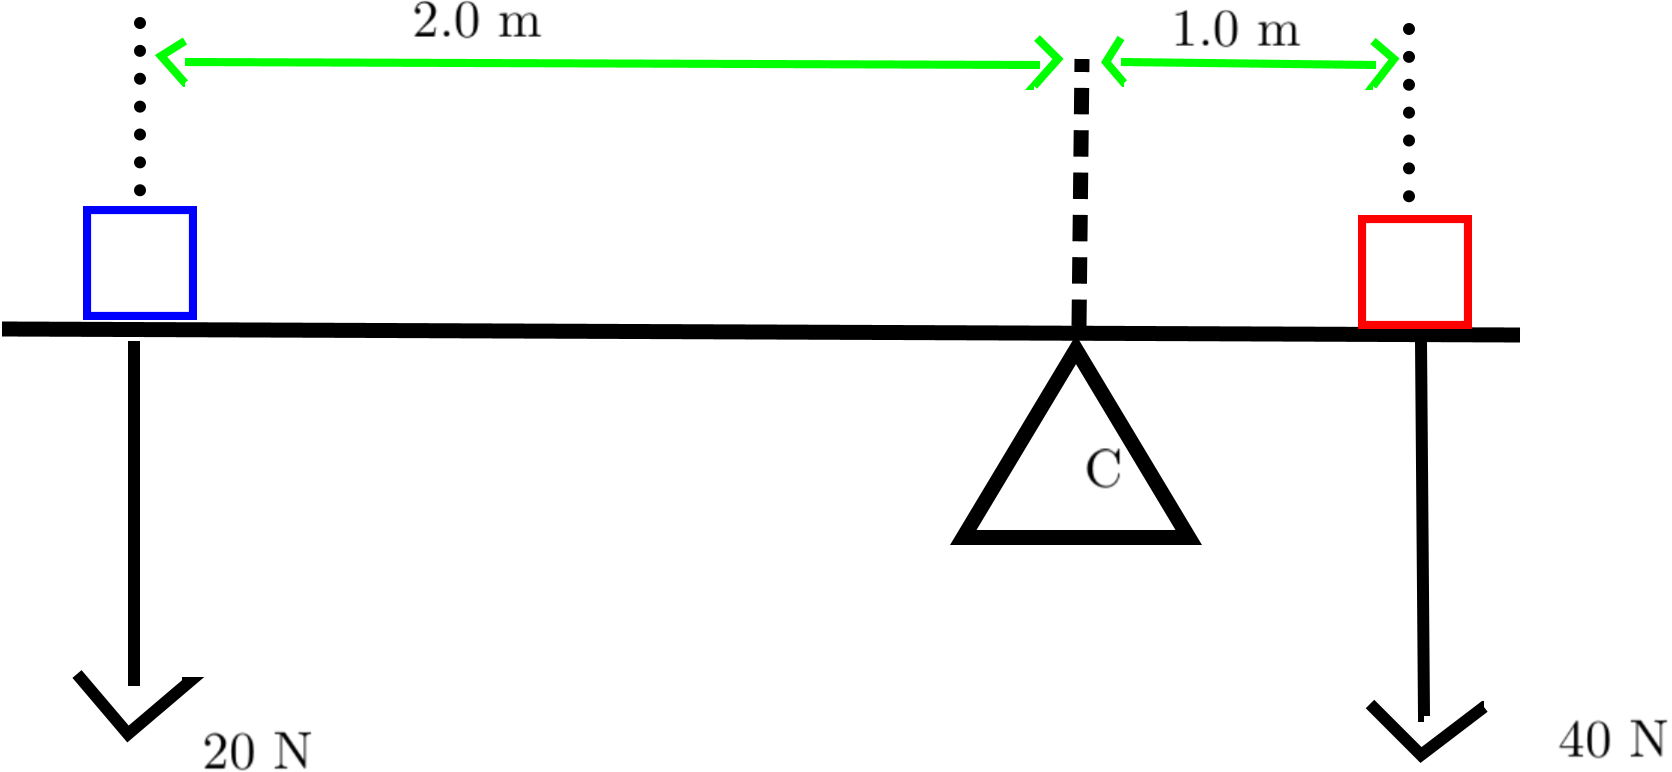
\includegraphics[width=50mm]{Imazhet/momenti.png}
		\caption{Momenti.}
		\label{fig:boat1}
	\end{figure}
	
	Për të gjetur momentin e forcave kemi:
	
	$\vec{M}$= $\vec{F}$ $\cdot$ $l$
	
	Nëse kemi ekuilibër kemi formulën:
	
	$(F_1 \cdot l_1 = F_2 \cdot l_2)$
	
	Dhe forca rezultante:
	
	$F_R =F_2-F_1$
	
	\textbf{7.4 Momenti rezultant.}
	
	$M_R=\vec{M_o}+\vec{M_{ko}}$
	
	Momenti Rezultant = Momenti orar pra momenti i forcave në krahun e majtë -
	Momentin në krahun kundër orar në krahun e djathtë.
	
	
	
	
	$M_R=(M_1+M_2)-(M_3+M_4)$
	
	
	\section{Gazet}
	
	\begin{center}
		Ekuacioni i gazeve.
	\end{center}
	
	$P \cdot V =n \cdot R \cdot T$
	
	\begin{center}
		Energjia kinetike.
	\end{center}
	
	$E_k=\frac{3}{2} \cdot k_B \cdot T$
	
	\begin{center}
		Energjia e brëndëshme.
	\end{center}
	
	U= $\frac{3}{2}$ $\cdot R \cdot T \cdot n $ 1 atom.
	
	U= $\frac{5}{2}$ $\cdot R \cdot T \cdot n $ 2 atom.
	
	U= 3$\cdot$ $\cdot R \cdot T \cdot n $ 3 atom.\\
	
	
	\textbf{8.1 Procesi izotermik.}
	
	Në procesin izotermik T(Temperatura) është konstante pra T = konstante dhe dy
	madhësit e tjera P(Presioni) dhe V (Vëllimi) janë në përpjestim të drejtë.
	
	$\frac{P_1}{P_2}$=$\frac{V_2}{V_1}$ $\Rightarrow$ $P_1 \cdot V_2=P_2 \cdot V_1$
	
	\begin{figure}[h]
		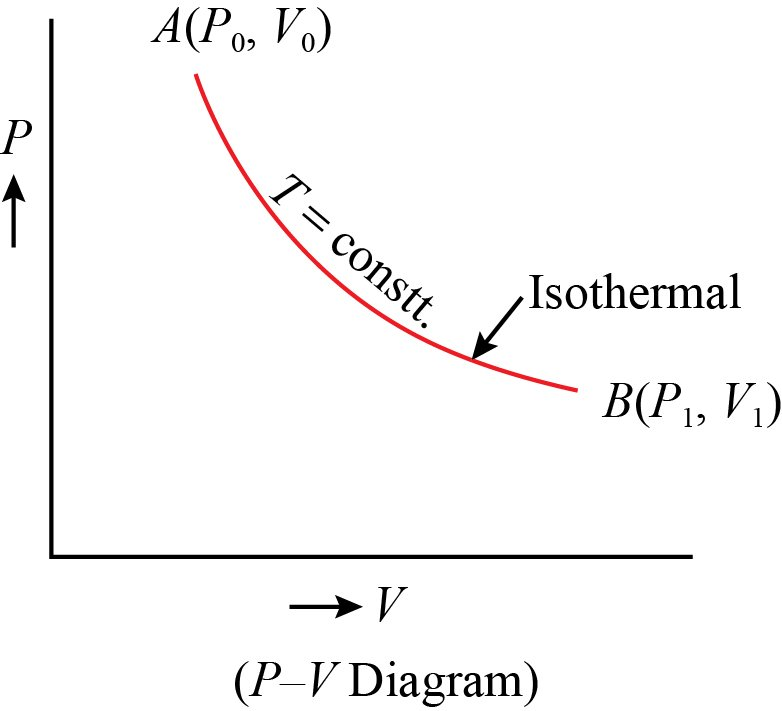
\includegraphics[width=40mm]{Imazhet/procesi_izotermik.jpg}
		\caption{Procesi izotermik.}
		\label{fig:boat1}
	\end{figure}
	
	\textbf{8.2 Procesi izohorik.}
	
	Në procesin izohorik V (Vëllimi) është konstante pra V = konstante dhe dy madhësit e
	tjera P(Presioni) dhe T(temperatura) janë në përpjestim të drejtë.
	
	\begin{figure}[h]
		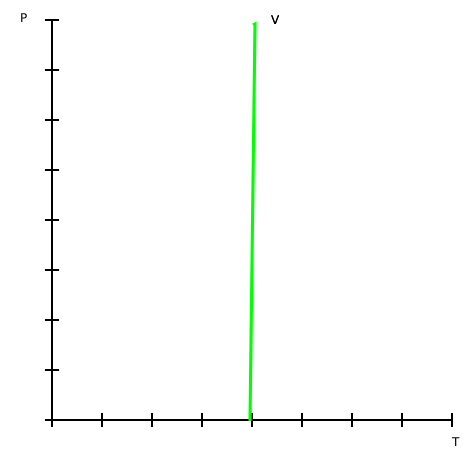
\includegraphics[width=30mm]{Imazhet/procesi izohorik.png}
		\caption{Procesi izohorik.}
		\label{fig:boat1}
	\end{figure}
	
	\begin{figure}[h]
		\includegraphics[width=40mm]{Imazhet/procesi izohorik1.png}
		\caption{Procesi izohorik.}
		\label{fig:boat1}
	\end{figure}
	
	$\frac{P_1}{P_2}$=$\frac{T_1}{T_2}$ $\Rightarrow$ $P_1 \cdot T_2=P_2 \cdot T_1$\\
	
	\textbf{8.3 Procesi izobarik.}
	
	Në procesin izobarik P(Presioni) është konstante pra P = konstante dhe dy madhësit
	e tjera V (Vëllimi) dhe T(temperatura) janë në përpjestim të drejtë.
	
	\begin{figure}[h]
		\includegraphics[width=40mm]{Imazhet/procesi izobarik.png}
		\caption{Procesi izobarik.}
		\label{fig:boat1}
	\end{figure}
	
	$\frac{T_1}{T_2}$=$\frac{V_1}{V_2}$ $\Rightarrow$ $T_1 \cdot V_2=T_2 \cdot V_1$\\
	
	\section{Inercia.}
	
	
	
	\begin{center}
		\textit{Simbolet:}
	\end{center}
	
	$M \Rightarrow$ Momenti.
	
	$m \Rightarrow $ Masa.
	
	$r \Rightarrow$ Rrezja.
	
	$\xi \Rightarrow $ Nxitimi këndor.
	
	$I \Rightarrow$ Inercia.
	
	$\omega \Rightarrow$ Shpejtësia këndore.
	
	$l \Rightarrow$ Rruga.
	
	$L \Rightarrow$ Momenti këndor.
	
	$\varphi \Rightarrow$ Zhvendosja.
	
	\begin{center}
		Formula:
	\end{center}
	
	$M= m \cdot r^2 \cdot \xi$
	
	$I= m \cdot r^2$
	
	$\xi=\frac{\omega - \omega_0}{t}$
	
	$M=\frac{L-L_0}{\Delta t}$=$\frac{\Delta L}{\Delta t}$
	
	$\omega=\omega_0 \pm \xi \cdot t$
	
	$\varphi = \omega_0 \cdot t \pm \frac{\xi \cdot t^2}{2}$
	
	$L=I\cdot \omega$
	
	\textbf{9.1 Disku i rrafshët.}
	
	$I= \frac{m \cdot r^2}{2}$\\
	
	\textbf{9.2 Unaza.}
	
	$I=m \cdot t^2$\\
	
	\textbf{9.3 Sfera.}
	
	$I=\frac{2 \cdot m \cdot t^2}{5}$\\
	
	\textbf{9.4 Cilindri.}
	
	$I= \frac{m \cdot r^2}{2}$\\
	
	\textbf{9.5 Shufra.}
	
	E mbështetur në fillimin e saj:
	
	$I=\frac{m \cdot l^2}{3}$
	
	E mbështetur në mesin e saj:
	
	$I=\frac{m \cdot l^2}{12}$
	
	
	\section{Impulsi.}
	
	\textbf{Impulsi:} produkti i masës me shpejtësin.
	
	\textbf{Ligji i ruajtjes së impulsit:} Në një sistem të mbyllur impulsi mbetet konstant.
	
	\textbf{Ligji i parë i Njutonit:} Një trup do të ruaj gjëndjen e vet të lëvizjes deri sa mbi të të veproj një forcë rezultante jo zero.
	
	\textbf{Ligji i dytë i Njutonit:} Nxitimi që fiton një trup nën veprimin e një force (rezultante) është në përpjestim të drejt me forcën dhe në përpjestim të zhdrejt me masën e trupit.
	
	\textbf{Ligji i tretë i Njutonit:} Forca me të cilat bashkveprojnë dy trupa kanë madhësi të barabarta dhe kahe të ndryshme.
	
	\begin{center}
		\textit{Simbolet:}
	\end{center}
	
	$p \Rightarrow $ Impulsi.
	
	$F \Rightarrow $ Forca.
	
	\begin{center}
		Formula:
	\end{center}
	
	$ p = m \cdot v$
	
	$F=\frac{\Delta p }{\Delta t}$\\
	
	
	Ligji i ruajtjes së impulsit(kur sistemi përbëhet nga dy trupa):
	
	$m_1 \cdot u_1 + m_2 \cdot u_2 =m_1 \cdot v_1 + m_2 \cdot v_2$
	
	\section{Puna.}
	
	\begin{center}
		\textit{Simbolet:}
	\end{center}
	
	$A$ ose $W \Rightarrow$ Puna $(Xhaul,J)$
	
	$S \Rightarrow $ Zhvendosja.
	
	$\mu \Rightarrow$ Konstante.
	
	$g \Rightarrow$ Konstante.
	
	$F \Rightarrow$ Forca.
	
	$E_p \Rightarrow $ Energjia potenciale.
	
	$E_k \Rightarrow$ Energjia kinetike.
	
	$P \Rightarrow $ Fuqia(Vat ,W).
	\begin{center}
		Formula:
	\end{center}
	
	$A=F_x \cdot S$
	
	$F_x=F \cdot $ cos$\theta$
	
	$A=F \cdot S \cdot$ cos$\theta$
	
	$A=-F \cdot S \cdot $ kur cos$\theta$=$180^\circ$
	
	$A=\mu\cdot m\cdot g-F \cdot $sin$\theta$ $\cdot$ $S$
	
	$E_p=m \cdot g \cdot h$
	
	$E_k=\frac{m \cdot v^2}{2}$
	
	$P=\frac{A}{t}$
	
	
	\textbf{Shënim:}
	
	$A>0$ kur $0 \leq \theta < 90^\circ$
	
	$A<0$ kur $ \theta > 90^\circ$
	
	$A=0$ kur $ \theta=90^\circ$
	
	\textbf{11.1 Puna e forcës së rëndesës(graviteti).}
	
	\begin{center}
		\textit{Simbolet:}
	\end{center}
	
	$A \Rightarrow $ Puna.
	
	$G \Rightarrow$ Forca e gravitetit.
	
	$h \Rightarrow$ Zhvendosja vertikale.
	
	$g \approx 9,8 m/s^2 \Rightarrow$ Konstante.
	\begin{center}
		Formula:
	\end{center}
	
	$A=G \cdot h$
	
	$G=m \cdot g$
	
	$A=m \cdot g \cdot h$
	
	\textbf{11.2 Puna e forcave elastike.}
	
	\begin{center}
		\textit{Simbolet:}
	\end{center}
	
	$A \Rightarrow $ Puna.
	
	$x \Rightarrow $ Shformimi ne metër.
	
	$k \Rightarrow $ Koeficenti i shformimit.
	
	$A_p \Rightarrow$ Puna e përgjithshme.
	
	\begin{center}
		Formula:
	\end{center}
	
	$A=\frac{k \cdot x^2}{2}$
	
	$A_p=A_F+A_f \Rightarrow A_p=A_F-A_f-A_{jashteme}$
	
	\textbf{11.3 Puna e Gazit(Pistoni).}
	
	\begin{center}
		\textit{Simbolet:}
	\end{center}
	
	$A \Rightarrow $ Puna.
	
	$p \Rightarrow $ Trysnia.
	
	$V \Rightarrow$  Vëllimi.
	
	\begin{center}
		Formula:
	\end{center}
	
	$A=p(V_2-V_1)$
	
	\section{Lënda dhe materialet.}
	
	Dendësia:masa e njësis së vëllimit të një materiali.
	
	Shtypje:forca që vepron pingule me njësinë e sipërfaqes.
	
	Shformimi: zgjatja e njësisë së gjatësis.
	
	Sforcimi: forca mbi njësinë e sipërfaqes së prerjes tërthore të matrialit.
	
	Modul i Jangut: raporti i sforcimit me shformimin e materialit kur ai i bindet ligjit të Hukut.
	
	\begin{center}
		\textit{Simbolet:}
	\end{center}
	
	$\rho$ $\Rightarrow$ Dendësia.
	
	$P \Rightarrow$ Shtypja.
	
	$P_b \Rightarrow $ Shtypja brënda lëngut.
	
	$\sigma \Rightarrow$ Sforcimi.
	
	$\epsilon \Rightarrow $ Shformimi.
	
	$E \Rightarrow$ Moduli i Jangut.
	
	$E_{pe} \Rightarrow $ Energjia potenciale elastike.
	
	\begin{center}
		Formula:
	\end{center}
	
	$\rho = \frac{m}{v}$
	
	
	$P = \frac{F}{S}$
	
	$P_b= \rho \cdot g \cdot h$
	
	$\sigma = \frac{F}{S}$
	
	$\epsilon = \frac{x}{L}$
	
	$E=\frac{\sigma}{\epsilon}$
	
	$E_{pe}=\frac{F\cdot x}{2}=\frac{kx^2}{2}$
	
	
	
	
	
	\section{Elektriciteti.}
	Në fizikë ngarkesat ndahen në ngarkesa pozitive dhe ngarkesa negative.
	
	\textbf{Ngarkesat pozitive:}
	Ngarkesat pozitive shënohen me (+) dhe grimcat shtyhen.Nëse kemi dy grimca një
	negative dhe një pozitive ato tërhiqen ndërsa kur dy grimca janë (+) ato shtyhen.
	
	\textbf{Ngarkesat negative:}
	Ngarkesat negative shënohen me (-) dhe grimcat tërhiqen.Nëse kemi dy grimca një
	negative dhe një pozitive ato tërhiqen ndërsa kur dy grimca janë (-) ato shtyhen.
	
	\begin{center}
		\textit{Simbolet:}
	\end{center}
	
	$E \Rightarrow $ Intesiteti i fushës.
	
	$F \Rightarrow $ Forca.
	
	$q_o \Rightarrow $ Ngarkesa "spihune".
	
	$r \Rightarrow $ Rrezja.
	
	$k \approx 9\cdot10^9 \Rightarrow $ Konstanet.
	
	\begin{center}
		Formula:
	\end{center}
	
	$E=\frac{F}{q_0}$
	
	$E= k \cdot \frac{q}{r^2}$\\
	
	\textbf{13.1 Forcat elektrike(Ligji i Kulonit).}
	
	\begin{center}
		\textit{Simbolet:}
	\end{center}
	
	$F_e \Rightarrow $ Forca elektrike.
	
	$\epsilon \Rightarrow $  Përshkrueshmëria e mjedisit.
	
	$k \Rightarrow $ Konstante.
	
	\begin{center}
		Formula:
	\end{center}
	
	$|\vec{F_e}|=k \cdot \frac{q_1 \cdot q_2}{r^2}$
	
	$|\vec{F_e}|=k \cdot \frac{Q \cdot q_0}{r^2}$
	
	$\vec{E}=k \cdot \frac{Q}{r^2}$ Në boshllëk.
	
	$\vec{E}=k \cdot \frac{Q}{\epsilon \cdot r^2}$ Në një mjedis.
	
	$k=\frac{1}{4 \pi \cdot \epsilon}$\\
	
	
	\textbf{13.2 Puna e forcave elektrike.}
	\begin{center}
		\textit{Simbolet:}
	\end{center}
	
	$A_e \Rightarrow $ Puna e forcave elektrike.
	
	$F \Rightarrow $ Forca.
	
	$d \Rightarrow $ Largëia.
	
	$E \Rightarrow $ Intesiteti i fushës.
	
	$q_o \Rightarrow $ Ngarkesa "spihune".
	
	\begin{center}
		Formula:
	\end{center}
	
	$A=F \cdot d$
	
	$E=\frac{F}{q_0}$
	
	$F=q_0 \cdot E$
	
	$A=q_0 \cdot E \cdot d$
	
	$A=-q_0 \cdot \Delta V$
	
	
	
	
	\textbf{13.3 Energjia potenciale.}
	
	\begin{center}
		\textit{Simbolet:}
	\end{center}
	
	$A_e \Rightarrow $ Puna e forcave elektrike.
	
	$W_p \Rightarrow$ Energjia potenciale elektrike.
	
	$V \Rightarrow$ Potenciali.
	
	$q \Rightarrow $ Ngarkesa e grimcës.
	
	$q_o \Rightarrow $ Ngarkesa "spihune".
	
	$r \Rightarrow $ Rrezja.
	
	\begin{center}
		Formula:
	\end{center}
	
	$A_e=-\Delta W_p$ $\Rightarrow$  $A_e=-(W_{p2}-W_{p1})$
	
	$V=\frac{W_p}{q_0}$
	
	$V=k \cdot \frac{Q}{r} \Rightarrow W_p=q_0 \cdot V$
	
	$A=-q_0 \cdot \Delta V$\\
	
	
	\textbf{13.4 Kondesatoret.}
	
	Kondensatori ose kapacitori është një element që përbëhet prej dy pllakave përçuese të veçuara me një jopërçues që quhet dielektrik. Nëse këto pllaka përçuese kanë potenciale të ndryshme, në mes tyre do të grumbullohet një sasi elektriciteti. 
	
	\begin{center}
		\textit{Simbolet:}
	\end{center}
	
	$C \Rightarrow $ Kapaciteti.$(Farad,F)$
	
	$Q \Rightarrow$ Ngarkesa e fushës.
	
	$U \Rightarrow $ Tensioni.
	
	$r \Rightarrow$ Rrezja.
	
	$k \Rightarrow $ Konstante. ($k=\frac{1}{4 \pi \cdot \epsilon_0}$)  
	
	$A$ ose $W \Rightarrow $ Puna në kondesator.
	
	$d \Rightarrow $ Largësia.
	
	$S \Rightarrow $ Sipërfaqa.
	
	$\epsilon_0 \Rightarrow$ Konstante.
	
	$\epsilon \Rightarrow $ Përshkrueshmëria e mjedisit.
	
	
	
	\begin{center}
		Formula:
	\end{center}
	
	$C=\frac{Q}{V}$
	
	$C=\frac{Q}{U}$
	
	$Q=C \cdot U$
	
	$C=\frac{R}{k}\Rightarrow R \cdot 4\pi \cdot \epsilon_0$ Për sferën.
	
	$C=\epsilon_0 \cdot \frac{S}{d}$ Në vakum.\\
	
	
	$C=\epsilon_0 \cdot \frac{S}{d} \cdot \epsilon$ Në një mjedis.
	
	$A=\frac{Q\cdot V}{2}$ Puna e kryer për ngarkimin e kondesatorit.
	
	$A=\frac{c \cdot u^2}{2}$ Puna e kryer për ngarkimin e kondesatorit.
	
	$A=\frac{Q^2}{2\cdot U}$ Puna e kryer për ngarkimin e kondesatorit.
	
	$A=Q \cdot U$ Puna që kryhet për të zhvendosur ngarkesën Q.
	
	\textbf{13.5 Lidhja e kondesatorëve. }
	
	\begin{center}
		\textbf{Lidhja në seri.}
	\end{center}
	
	\begin{figure}[h]
		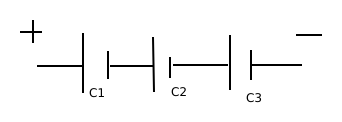
\includegraphics[width=50mm]{Imazhet/Lidhjet ne seri.png}
		\caption{ Lidhja e kondesatorëve në seri.}
		\label{fig:boat1}
	\end{figure}
	
	\textbf{1-$Q$(ngarkesa) është konstante.}
	
	$Q_1=Q_2=Q_3=Q_n$
	
	\textbf{2-$U$(Tensioni).}
	
	$U=U_1+U_2+U_3+U_n$
	
	\textbf{3-$C$(Kondesatorët).}
	
	$\frac{1}{C_p}=\frac{1}{C_1}+\frac{1}{C_2}+\frac{1}{C_3}+\frac{1}{C_n}$
	
	
	\begin{center}
		\textbf{Lidhja paralele.}
	\end{center}
	\begin{figure}[h]
		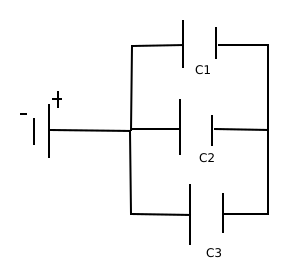
\includegraphics[width=30mm]{Imazhet/Lidhjet paralele.png}
		\caption{ Lidhja e kondesatorëve në paralel.}
		\label{fig:boat1}
		
		
	\end{figure}
	
	\textbf{1-$Q$(ngarkesa).}
	
	$Q=Q_1+Q_2+Q_3+Q_n$\\
	
	\textbf{2-$U$(Tensioni) është konstant.}
	
	$U_1=U_2=U_3=U_n$\\
	
	\textbf{3-$C$(Kondesatorët).}
	
	
	$C_p=C_1+C_2+C_3$\\
	
	\textbf{13.6 Rryma elektrike.}
	
	Rryma elektrike është rrjedhje e ngarkesave elektrike. Në qarqe elektrike kjo ngarkesë zakonisht realizohet nga lëvizja e elektroneve në një kabllo. Ajo mund të realizohet nga jonet në një elektrolitë, ose nga të dyja jonet dhe elektronet si në një plazmë.
	
	Njësia për matjen e rrymës elektrike në sistemin SI është amperi, që është rrjedhja e ngarkesës elektrike rreth një sipërfaqeje në vlerë prej 1 kuloni për sekond. Rryma elektrike matet me anë të një pajisjeje që quhet ampermetër.
	
	
	\begin{flushleft}
		\textbf{	Rryma e ngarkuar e vazhduar.}
	\end{flushleft}
	\begin{figure}[h]
		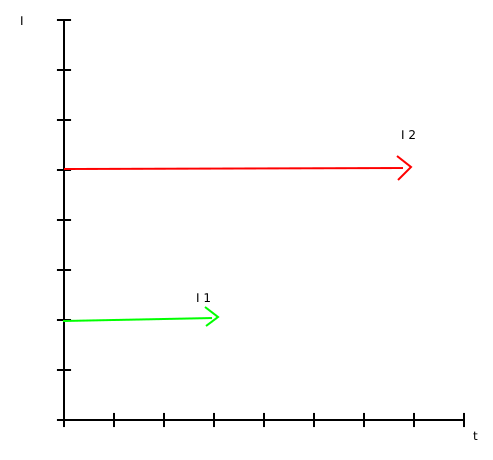
\includegraphics[width=50mm]{Imazhet/rryma e ngarkuar e vazhduar.png}
		\caption{Rryma e ngarkuar e vazhduar(Grafiku) $I_2>I_1$.}
		\label{fig:boat1}
	\end{figure}
	
	
	\begin{flushleft}
		\textbf{	Rryma alternative.}
	\end{flushleft}
	\begin{figure}[h]
		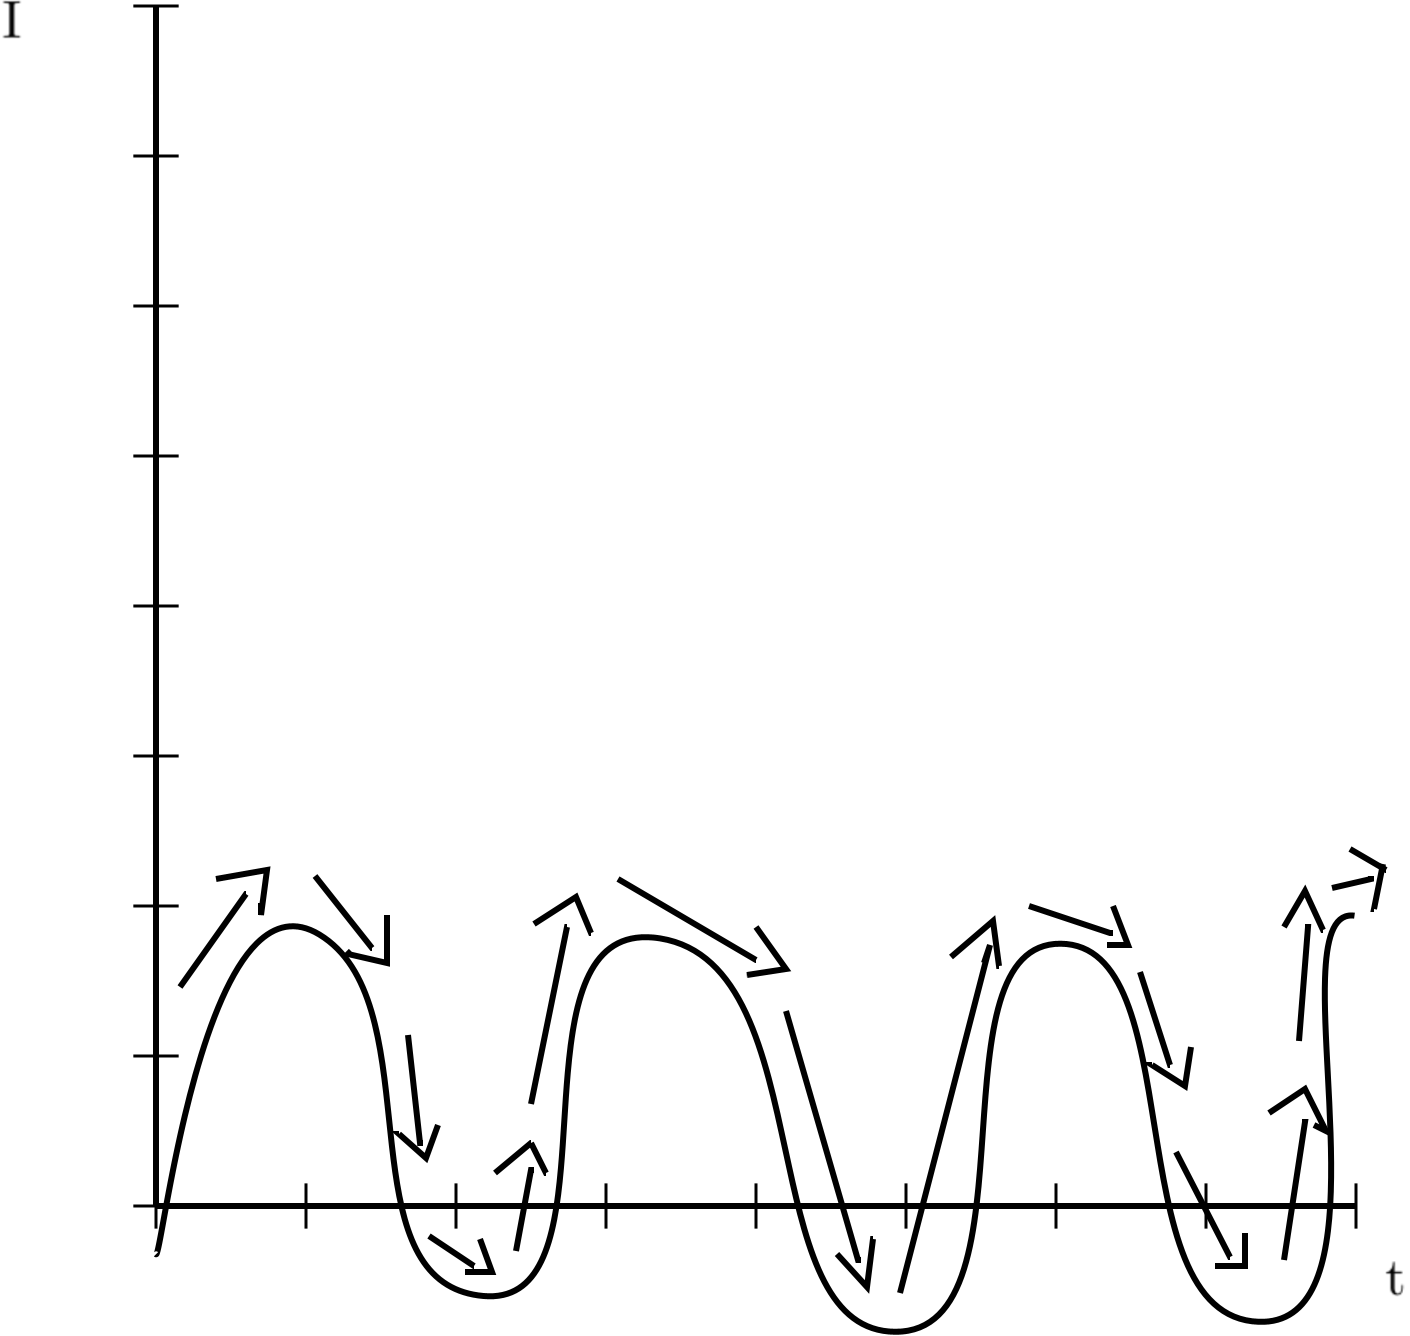
\includegraphics[width=45mm]{Imazhet/Rryma alternative.png}
		\caption{Rryma alternative(Grafiku).}
		\label{fig:boat1}
	\end{figure}
	
	\begin{center}
		\textit{Simbolet:}
	\end{center}
	
	$I \Rightarrow $ Rryma.$(Amper,A)$
	
	$j \Rightarrow $ Dendësia e rrymës.($\frac{A}{m^2}$)
	
	$q \Rightarrow$ Ngarkesa elektrike.$(Kulon,c)$
	
	$t \Rightarrow $ Koha. 
	
	$S \Rightarrow $ Sipërfaqa.
	\begin{center}
		Formulat:
	\end{center}
	
	$I=\frac{\Delta q}{\Delta t}$\\
	
	
	$j=\frac{I}{S}$\\
	
	
	\textbf{13.7 Burimi i rrymës.}
	\begin{figure}[h]
		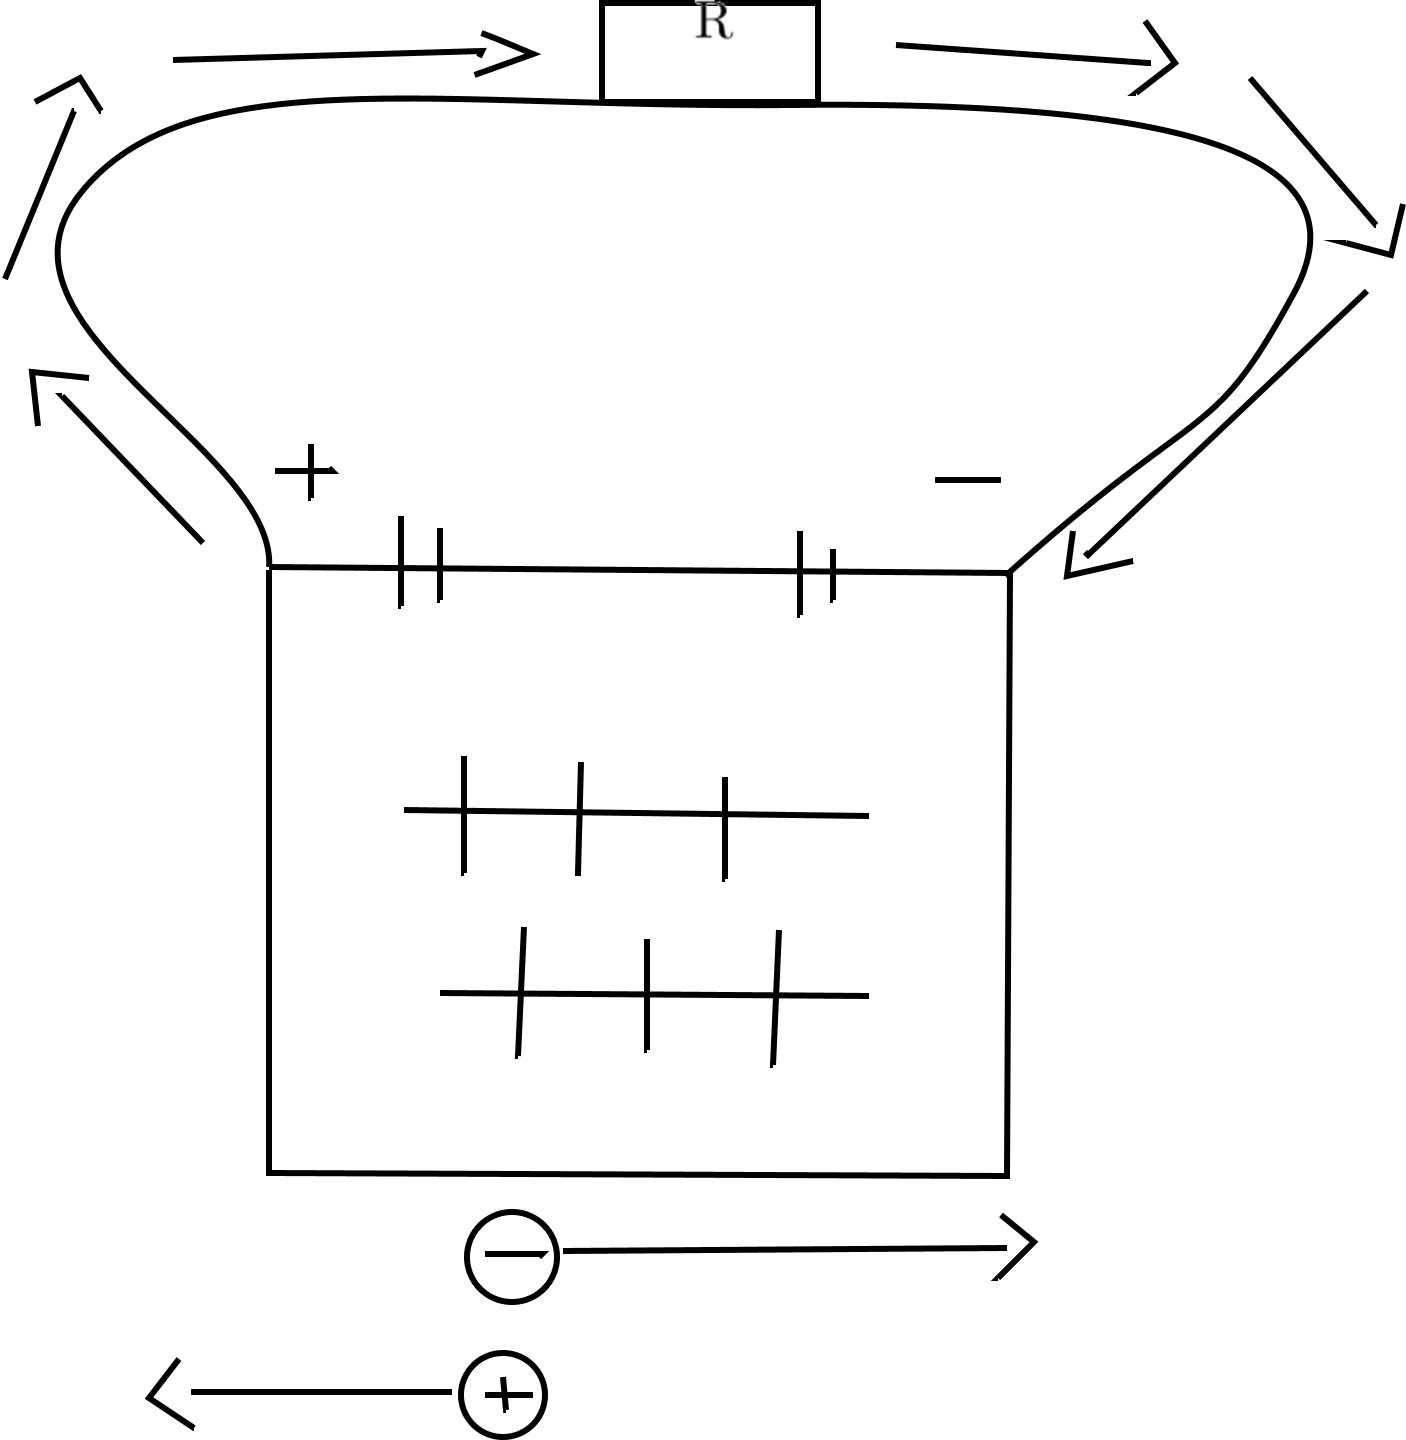
\includegraphics[width=50mm]{Imazhet/bateria.png}
		\caption{Burimi i rrymës (Bateria).}
		\label{fig:boat1}
	\end{figure}
	
	\begin{center}
		Simbolet:
	\end{center}
	
	$R \Rightarrow $ Rezistenca.
	
	$\rho \Rightarrow$ Rezistenca specifike.
	
	$l \Rightarrow $ Largësia.
	
	$S \Rightarrow $ Sipërfaqa.
	
	$\epsilon \Rightarrow $ Forca elektromotore.
	
	$A_b \Rightarrow$ Puna e brendëshme.
	
	$q \Rightarrow $ Ngarkesa.
	
	$\alpha \Rightarrow $ Koeficenti termik.
	
	$t \Rightarrow $ Temperatura.
	
	\begin{center}
		Formula:
	\end{center}
	
	$R=R_0[1+\alpha(t-t_0)]$\\
	
	$R= \rho \cdot \frac{l}{S}$\\
	
	$\rho=\rho_0 [1+\alpha(t-t_0)]$\\
	
	
	\textbf{13.8 Shndërrimet energjitike.}
	
	\begin{center}
		\textbf{	Ligji i Omit.}
	\end{center}
	
	\textbf{1-Ligji i Omit për një pjesë homogjene.}
	
	\begin{center}
		\textit{Simbolet:}
	\end{center}
	
	$I \Rightarrow $ Rryma elektrike.
	
	$U \Rightarrow $ Tensioni.
	
	$R \Rightarrow $ Rezistenca.
	
	\begin{center}
		Formula:
	\end{center}
	
	$I=\frac{U}{R}$\\
	
	\textbf{2-Ligji i Omit për qarkun e plotë.}
	
	\begin{center}
		\textit{Simbolet:}
	\end{center}
	
	$I \Rightarrow $ Rryma elektrike.
	
	$U \Rightarrow $ Tensioni jashtëm.
	
	$R \Rightarrow $ Rezistenca e jashtëme.
	
	$\epsilon \Rightarrow$ Përcjellësi.
	
	$r \Rightarrow $ Rezistenca e brëndshme.
	
	$u \Rightarrow $ Tensioni i brëndshem.
	
	
	
	\begin{center}
		Formula:
	\end{center}
	
	$I=\frac{\epsilon}{R+r}$ 
	
	$\epsilon=I \cdot (R+r)$
	
	$\epsilon=U+u$
	
	$I=\frac{\epsilon}{R}$
	
	\begin{center}
		\textbf{	Ligji i Xhaul Lencit.}
	\end{center}
	
	\begin{center}
		\textit{Simbolet:}
	\end{center}
	
	$Q \Rightarrow $ Energjia e çliruar $(Xhaul,J)$.
	
	$I \Rightarrow $ Rryma $(Amper ,A )$.
	
	$R \Rightarrow $ Rezistenca e përcjellësit.
	
	$t \Rightarrow$ Koha.
	
	$P \Rightarrow $ Fuqia.$(Vat,W)$
	
	$E \Rightarrow $ Energjia.$(Vat/sekond,W/s)$
	
	$N \Rightarrow $ Fuqia termike.
	
	$W \Rightarrow $ Fuqia mekanike.
	
	$\epsilon_k \Rightarrow $ Forca kundër elektromotore.
	
	$U \Rightarrow $ Tensioni.
	
	$I \cdot R \Rightarrow$ Tensioni në konsumator.
	\begin{center}
		Formula:
	\end{center}
	
	$Q=I^2 \cdot R \cdot t$
	
	$Q=I \cdot U \cdot t$
	
	$Q= P\cdot t$
	
	$P= I \cdot U$
	
	$E=\frac{P}{t}$
	
	$N=I^2 \cdot R$
	
	$W=I \cdot t$
	
	$\epsilon_k=\frac{W}{I \cdot t}$
	
	$U=I \cdot R + \epsilon_k$
	
	$I \cdot R =  U - \epsilon_k$\\
	
	\textbf{13.9 Lidhja e një qarku elektrik.}
	
	\begin{center}
		\textbf{Lidhja në seri.}
	\end{center}
	
	\begin{figure}[h]
		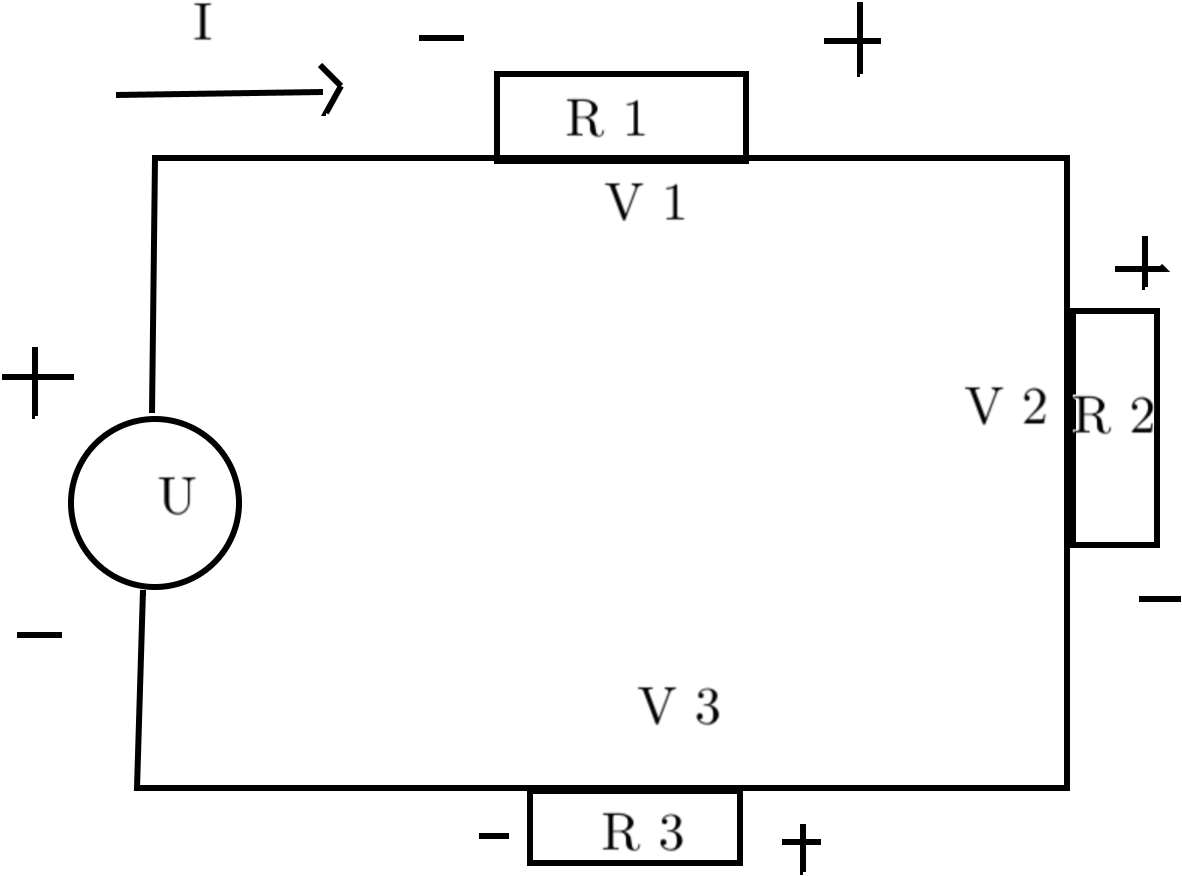
\includegraphics[width=45mm]{Imazhet/qarku seri.png}
		\caption{Lidhja e qarkut elektrik në seri.}
		\label{fig:boat1}
	\end{figure}
	
	\textbf{1-$I \Rightarrow $ Rryma është konstante.}
	
	$I_1=I_2=I_3=I_n$\\
	
	\textbf{2-$U$ $\Rightarrow$Tensioni.}
	
	$U=U_1+U_2+U_3+U_n$\\
	
	\textbf{3-$R \Rightarrow $ Rezistenca}
	
	$R=R_1+R_2+R_3+R_n$\\
	
	\textbf{4-$P \Rightarrow$ Fuqia.}
	
	$P=P_1+P_2+P_3+P_n$\\
	
	\begin{center}
		\textbf{Lidhja paralele.}
		
	\end{center}
	\begin{figure}[h]
		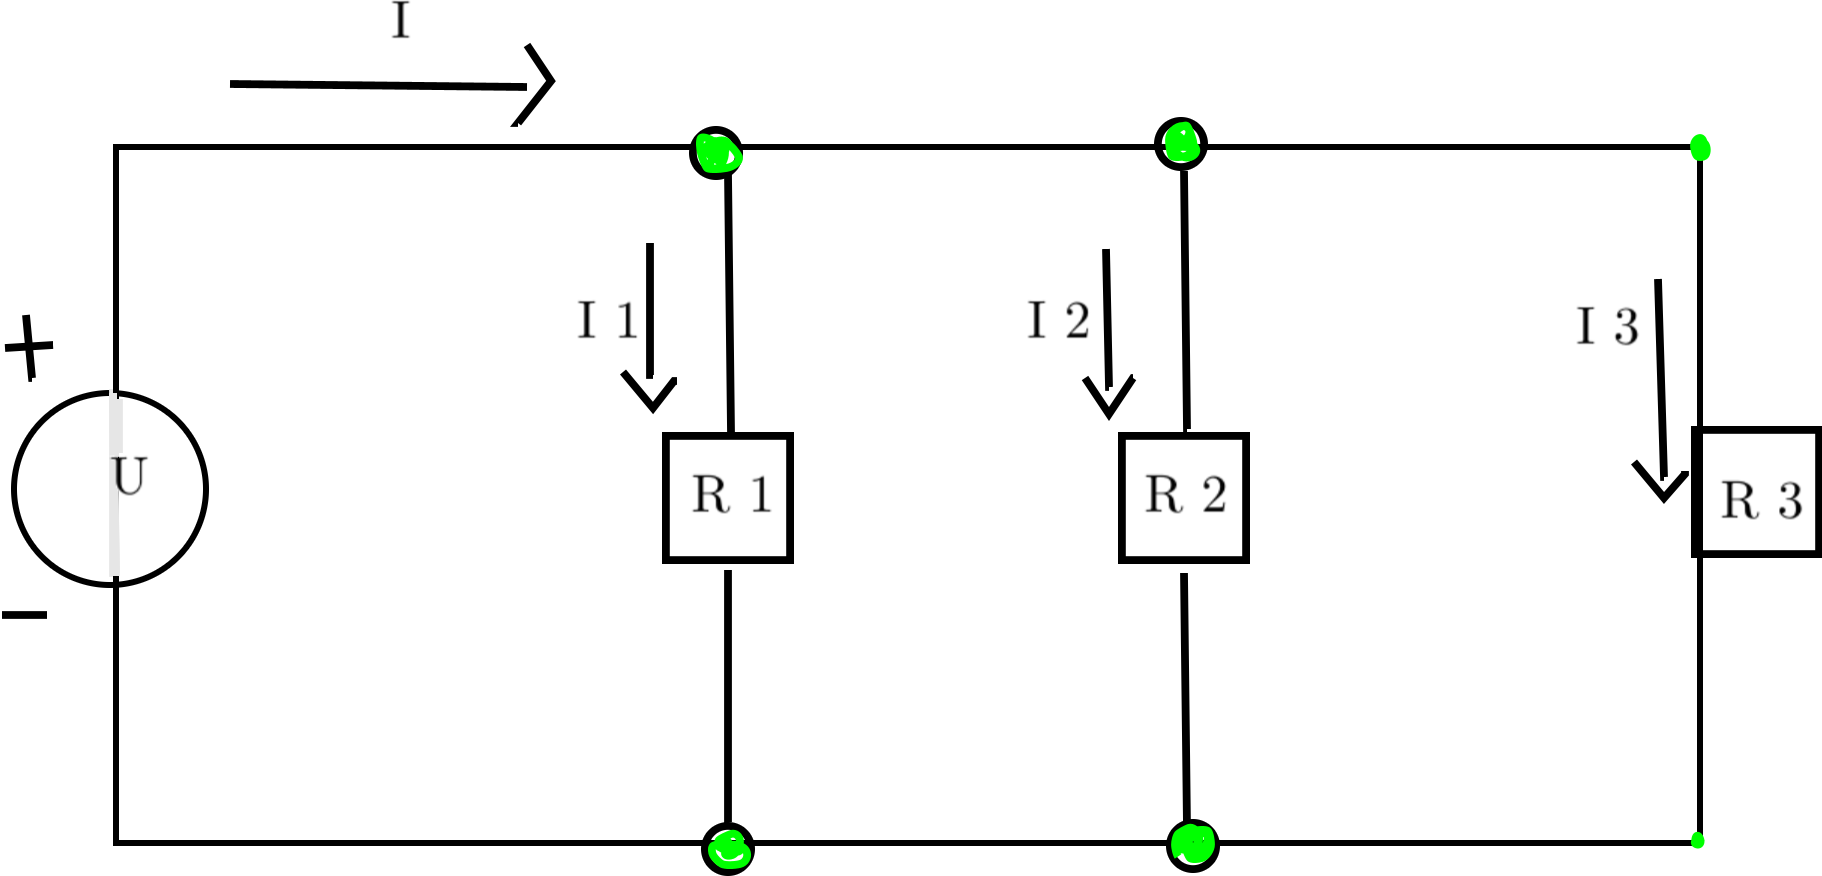
\includegraphics[width=55mm]{Imazhet/qarku paralel.png}
		\caption{Lidhja e qarkut elektrik paralel.}
		\label{fig:boat1}
	\end{figure}
	
	\textbf{1-$I \Rightarrow $ Rryma.}
	
	$I=I_1+I_2+I_3+I_n$\\
	
	\textbf{2-$U$ $\Rightarrow$Tensioni është konstant.}
	
	$U_1=U_2=U_3=U_n$\\
	
	\textbf{3-$R \Rightarrow $ Rezistenca}
	
	$\frac{1}{R_p}$=$\frac{1}{R_1}$+$\frac{1}{R_2}$+$\frac{1}{R_3}$+$\frac{1}{R_n}$\\
	
	\textbf{4-$P \Rightarrow$ Fuqia.}
	
	$P=P_1+P_2+P_3+P_n$\\
	
	\begin{center}
		\textbf{Lidhja e shkurtër.}
	\end{center}
	\begin{figure}[h]
		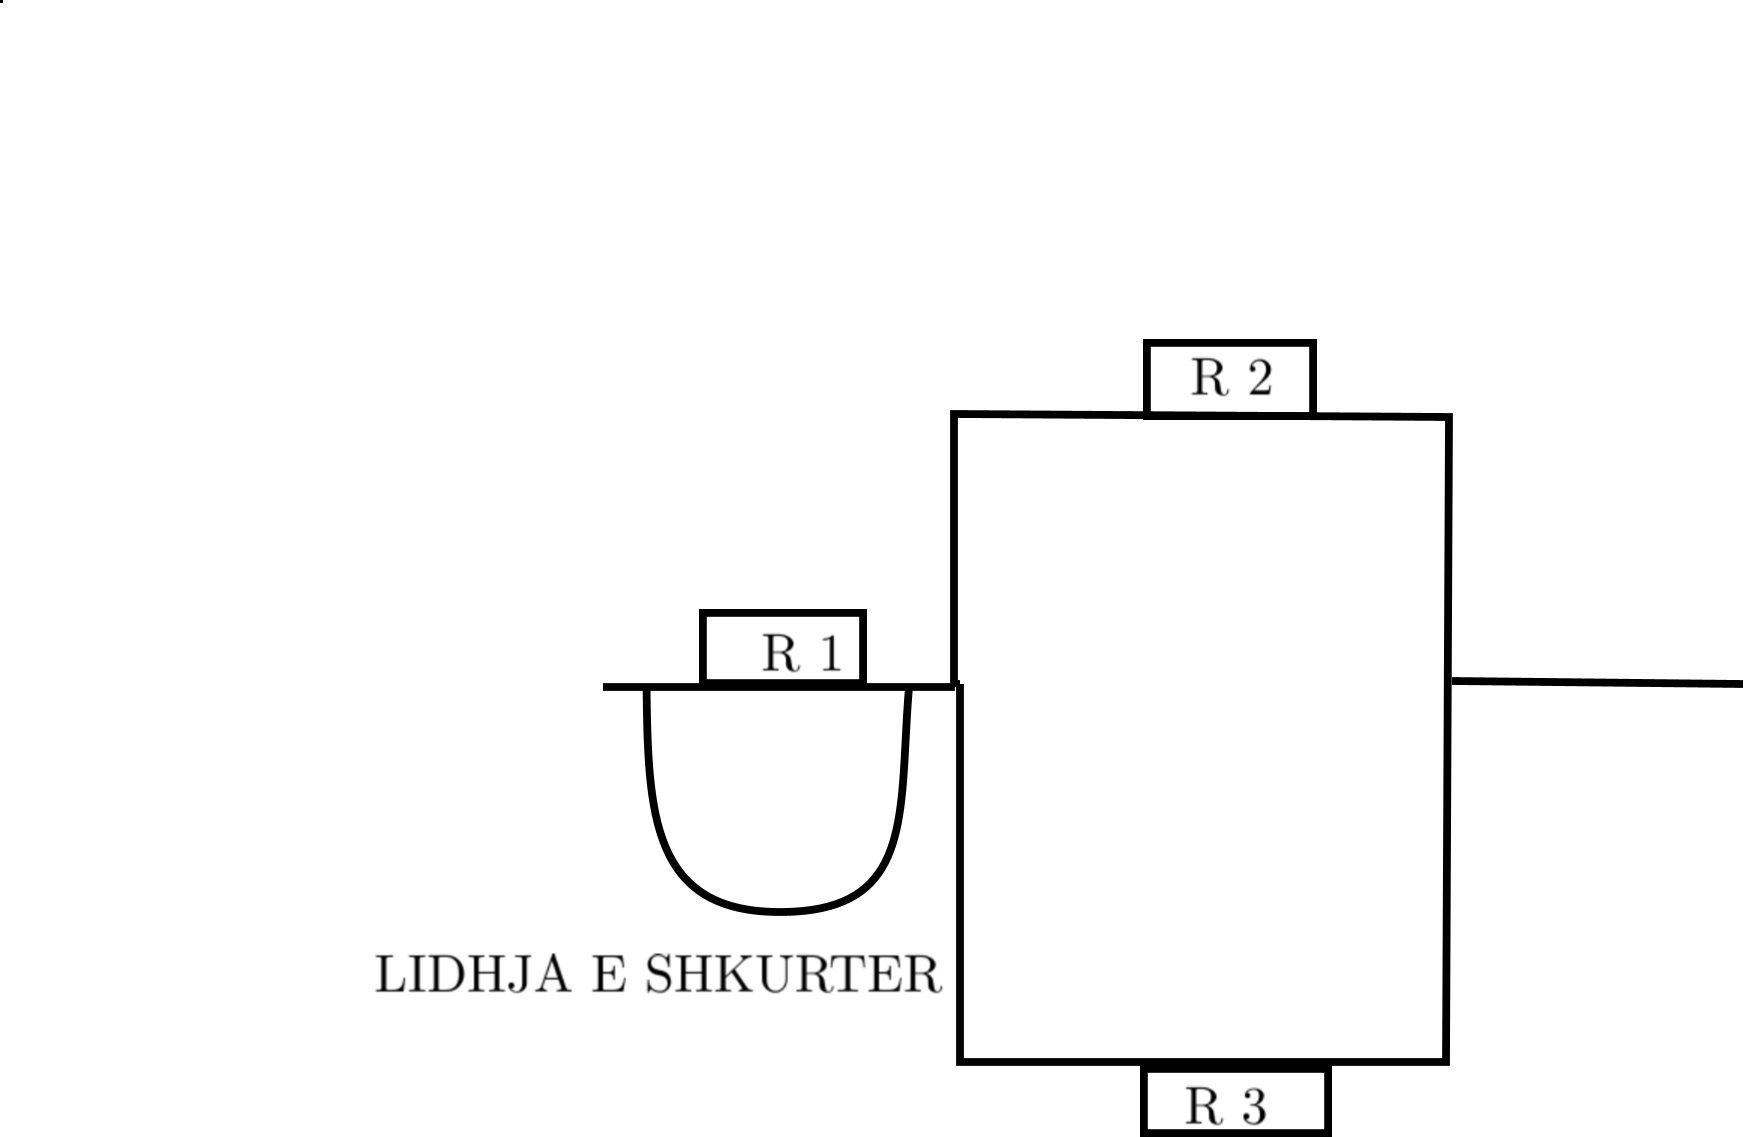
\includegraphics[width=60mm]{Imazhet/Lidhja e shkurter.png}
		\caption{Lidhja e shkurtër në një qark.}
		\label{fig:boat1}
	\end{figure}
	
	\section{Fusha magnetike.}
	\begin{figure}[h]
		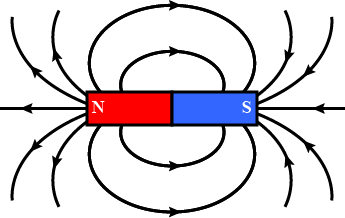
\includegraphics[width=50mm]{Imazhet/fusha_magnetike.png}
		\caption{Fusha magnetike e një magneti kuboid.}
		\label{fig:boat1}
	\end{figure}
	Në fizikë, një fushë magnetike është një fushë vektoriale që përshkon gjithë hapësirën dhe e cila shkakton një forcë magnetike mbi një ngarkesë elektrike lëvizëse ose mbi një dipol magnetik (siç janë magnetet e përhershëm). Kur vendoset në një fushë magnetike, dipoli magnetik tenton që të drejtohet sipas një boshti që është paralel me fushën magnetike, siç mund të shikohet edhe nga pluhuri i hekurit në prezencën e një magneti (shikoni pikturën në të djathte). Për më tepër, një fushë magnetike që ndrydhon në kohë shkakton induktimin e një fushë elektrike. Fushat magnetike rrethojnë dhe në të njëjtën kohë kanë si burim korrentet elektrike, dipolët magnetike, dhe fushat elektrike që ndryshojnë në kohë. Fushat magnetike mbartin energjinë e tyre, një denitet energjie e cila është në përpjesëtim të drejte me intensitetin e fushës.
	
	\begin{center}
		\textit{Simbolet:}
	\end{center}
	
	$B \Rightarrow $ Induksioni magnetik.$(Tesla,T)$
	
	$F_m \Rightarrow$ Forca magnetike.
	
	$l \Rightarrow$ Gjatësia.
	
	$\mu_0 = 4\pi \cdot 10^{-7} \Rightarrow $ Konstante.
	
	$d \Rightarrow $ Largësia.
	
	$R \Rightarrow$ Rezistenca.
	
	$n \Rightarrow $ Numri i spirave.
	
	\begin{center}
		Formula:
	\end{center}
	
	$B=\frac{F_m}{I \cdot l}$
	
	$F_m=I \cdot B \cdot \Delta l \cdot$ sin$\alpha$
	
	$B=\mu_0 \cdot \frac{I}{2 \pi \cdot d}$ Plani drejtvizor.
	
	$B=\mu_0 \cdot \frac{I}{2 \cdot R}$ Spira rrethore.
	
	$B=\mu_0 \cdot \frac{n \cdot I}{2 \cdot R}$ Bobina e ngusht.
	
	$B=\mu_0 \cdot \frac{n \cdot I}{l}$ Bobina e gjatë.
	
	$n=\frac{B}{e}$ Numri i spirave.
	
	\textbf{14.1 Fluksi magnetik.}
	
	\begin{figure}[h]
		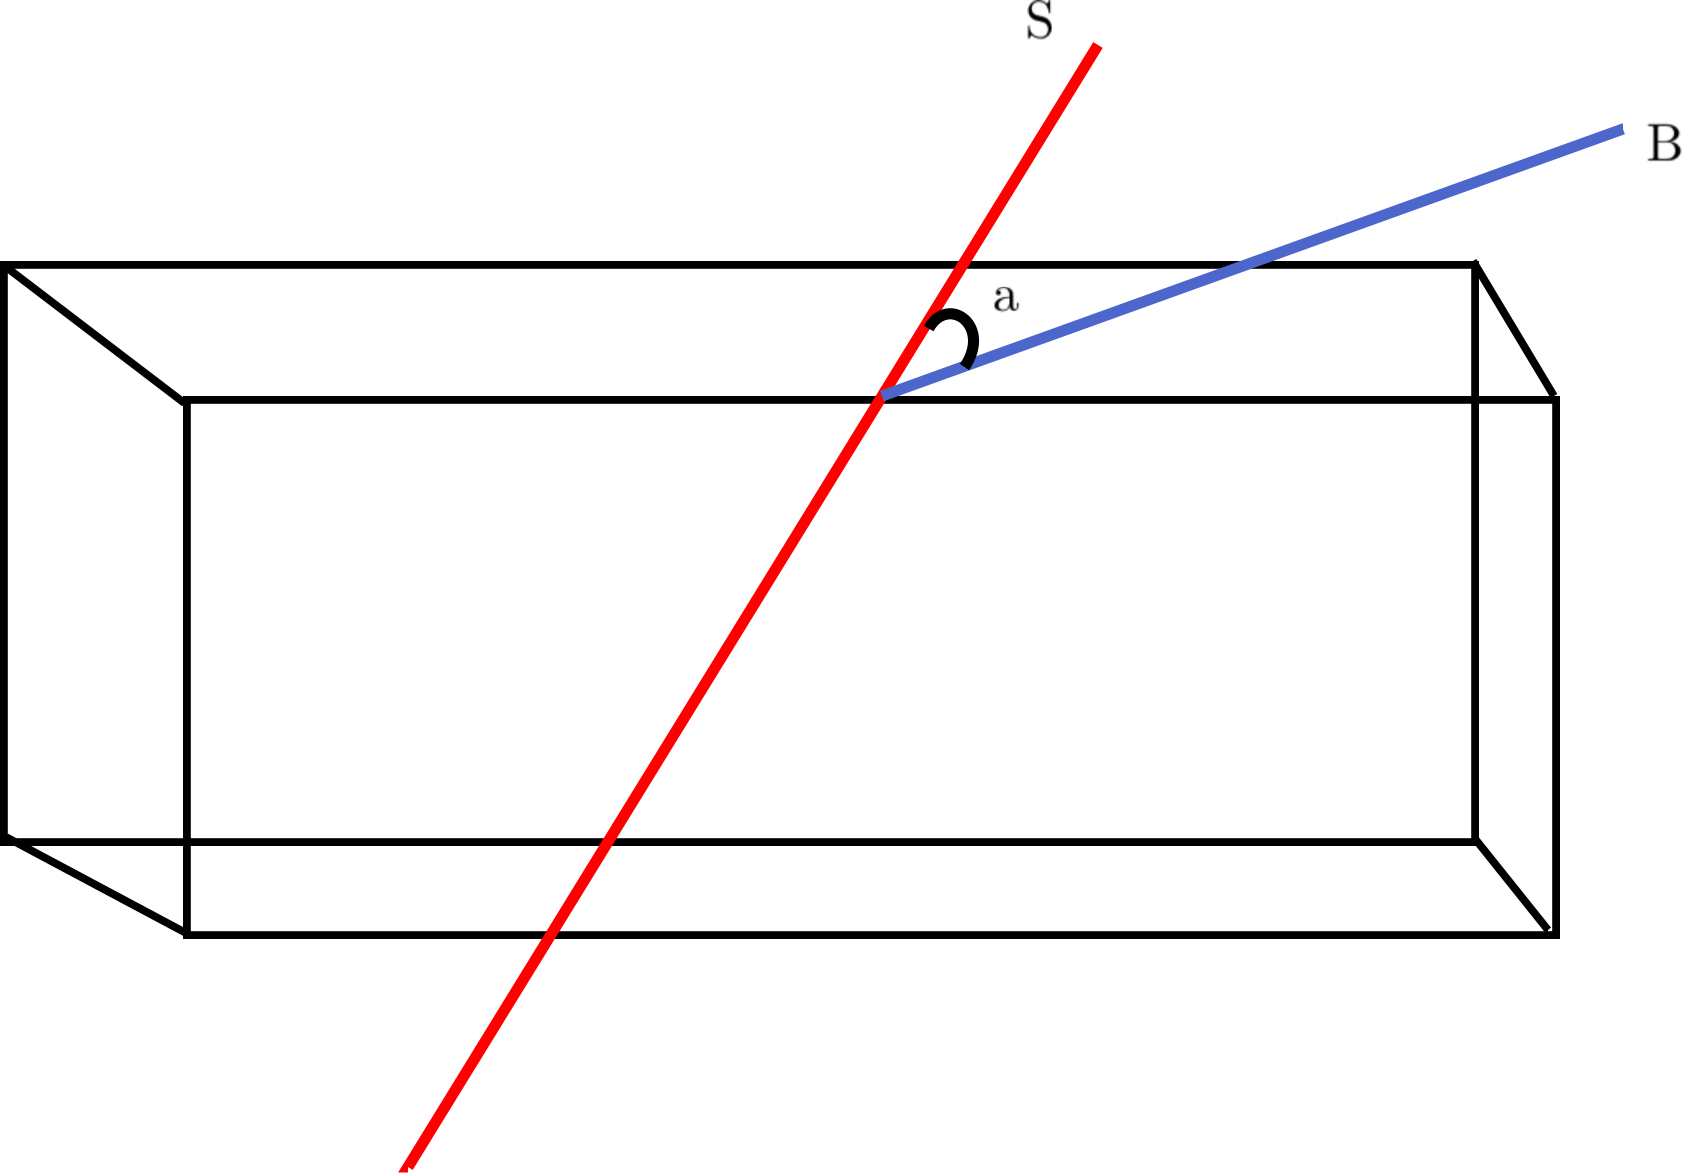
\includegraphics[width=60mm]{Imazhet/goditesi.png}
		\caption{Figura e fluksit magnetik.}
		\label{fig:boat1}
	\end{figure}
	
	1.$\phi= max$ kur $\alpha=0$ $B \parallel S$\\
	
	
	
	2.$\phi= 0$ kur $\alpha=90^\circ$ $B \perp S$
	\begin{center}
		\textit{Simbolet:}
	\end{center}
	
	$\phi \Rightarrow$Fluksi magnetik (Ëeber, $W_b$)
	
	$B \Rightarrow$ Induksioni magnetik.
	
	$S \Rightarrow $ Forca elektrike që ushtrohet.
	
	$\alpha \Rightarrow $ Këndi që formon $S$ me $B$.
	
	\begin{center}
		Formula:
	\end{center}
	
	$\phi$=$B \cdot S \cdot $sin$\alpha$\\
	
	\textbf{14.2 Mjediset magnetike.}\\
	
	Mjedise paramagnetik $\mu$ $\geq  1$\\
	
	Mjedise diamagnetik $\mu$ $\leq  1$\\
	
	Mjedise feromagnetik $\mu > 1$\\
	
	\begin{center}
		\textit{Simbolet:}\\
	\end{center}
	
	$\mu \Rightarrow $ Përshkrueshmëria.\\
	
	$B \Rightarrow $induksioni në një mjedis.\\
	
	$B_0 \Rightarrow $nduksioni në boshllëk.\\
	
	\begin{center}
		Formula:
	\end{center}
	
	$\mu=\frac{B}{B_0}$\\
	
	
	\textbf{14.3 Induksioni elektromagnetik(Ligji i Faradejt).}
	
	\begin{figure}[h]
		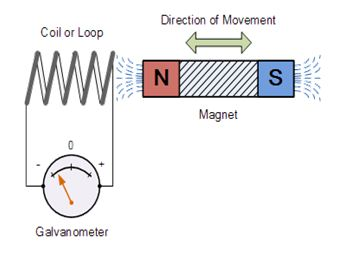
\includegraphics[width=60mm]{Imazhet/faraday law.jpg}
		\caption{Induksioni elektromagnetik.}
		\label{fig:boat1}
	\end{figure}
	
	Induksion elektromagnetik do të quajm dukruinë e përftimit të rrymës elektrike nga
	ndryshimi i fushës magnetike.
	
	$I_n \Rightarrow $ Rryma e induktuar.
	
	$\epsilon_n$ $\Rightarrow$ forca elektromotore e induktuar.
	
	
	\begin{center}
		Formula:
	\end{center}
	
	$I_n =-\Delta I_n$
	
	$\Delta I_n=I_2-I_1=B_2 \cdot S \cdot cos\alpha - B_1 \cdot S \cdot cos\alpha$\\
	
	\textbf{14.4 Fusha magnetike e Lencit.}
	
	\begin{center}
		\textit{Simbolet:}
	\end{center}
	
	$F_{Lencit} \Rightarrow $ Forca e Lencit.
	
	$q \Rightarrow $ Ngarkesa.
	
	$r \Rightarrow $ Rrezja.
	
	$B \Rightarrow $ Induksioni.
	
	$F_{q} \Rightarrow$  Forca qëndërsynuese.
	
	$m \Rightarrow $ Masa.
	
	$v \Rightarrow$ Shpejtësia.
	
	\begin{center}
		Formula:
	\end{center}
	
	$F_L=q  \cdot r \cdot sin\alpha$
	
	$F_q=\frac{m \cdot v^2}{r}$
	
	$F_q=F_L$ $\Rightarrow$ $\frac{m \cdot v^2}{R}=q \cdot v \cdot B \cdot sin\alpha$\\
	
	\textbf{14.5 Autoinduksioni. }
	
	\begin{center}
		\textit{Simbolet:}
	\end{center}
	
	$\phi \Rightarrow$ Autoinduksioni.
	
	$B \Rightarrow $ Induksioni.
	
	$S \Rightarrow $ Sipërfaqa.
	
	$I \Rightarrow $ Rryma.
	
	$L \Rightarrow$ Induktiviteti i qarkut.$(Henri,H)$
	
	$\epsilon_{au} \Rightarrow $ Forca elektromekatike e autoinduksionit.
	
	$W_m \Rightarrow $ Energjia magnetike.
	
	$\epsilon_{mt} \Rightarrow $ Forca elektromekanike.
	
	\begin{center}
		Formula:
	\end{center}
	
	$\phi =B \cdot S$
	
	
	$\phi =L \cdot I$
	
	
	$\epsilon_{au}=-L \cdot \frac{\Delta I}{\Delta t}$
	
	$W_m=\frac{L \cdot I^2}{2}$
	
	$\epsilon_{mt} = \frac{\phi_2 - \phi_1}{\Delta t}$$=$ $\frac{B_2 \cdot S \cdot r^2-B_1 \cdot S \cdot r^2}{\Delta t}$
	
	\section{Lëkundjet.}
	
	\begin{figure}[h]
		\includegraphics[width=80mm]{Imazhet/lekundjet.png}
		\caption{Lavjerrësi me vizatimet e forcave.}
		\label{fig:boat1}
	\end{figure}
	\begin{center}
		\textit{Simbolet:}
	\end{center}
	
	$T \Rightarrow$ Perioda.
	
	$f \Rightarrow $ Frekuenca(numri i lëkundjeve).
	
	$x \Rightarrow$ Madhësi fizike.
	
	$x_{(t)} \Rightarrow$ Madhësi fizike e cila ndryshon me kohën.
	
	$A \Rightarrow$ Amplituda(vlera më e madhe e lëkundjes).
	
	$\omega t \Rightarrow$ këndi i lëkundjes.
	
	$\varphi_0 \Rightarrow$ Faza fillestare.
	
	$x_s \Rightarrow $ Shormimi tek lavjerrësi sust.
	\begin{center}
		Formula:
	\end{center}
	
	$x_{(t)}=A \cdot cos(\omega t + \varphi) $ Ek.lëkundjes.
	
	\begin{center}
		\textbf{Lëvizja e një lavjerrësi.}
		
		$\omega$=$\frac{2 \pi}{T}$\\
		
		$\omega=2\pi \cdot f$\\
		
	\end{center}
	
	
	
	\begin{center}
		\textbf{Lavjerrësi sust.}\\
		
		$\omega=\sqrt{\frac{k}{m}}$\\
		
		$T=2\pi \cdot \sqrt{\frac{m}{k}}$
		
	\end{center}
	
	\begin{center}
		\textbf{Lavjerrësi matematik.}
	\end{center}
	\begin{flushleft}
		
		\textbf{\textit{Çfarë emërtojmë një lavjerrës matematik?}}\\
		
		
		Lavjerrësi matematik do të emërtojmë atë lavjerrës kur $l$(gjatësia e fillit) do të jetë shumë më e madhe se $r$(rrezja) e sferës.Dhe kur masa e fillit të jetë shumë herë më e vogël se sa masa e sferës që ajo ekuilibron. $g \approx 9,8 m/s^2$ (Konstante).
	\end{flushleft}
	
	
	$\omega=\sqrt{\frac{g}{l}}$
	
	$T=2\pi \cdot \sqrt{\frac{l}{g}}$
	
	\begin{center}
		\textbf{Lëkundjet në qarkun elektrik.}
		
		
	\end{center}
	
	$\omega=\sqrt{\frac{I}{L \cdot C}}$
	
	$T=2 \pi \cdot \sqrt{L \cdot C}$
	\begin{center}
		\textbf{Paraqitja grafike(lëkundja pa fazë).}\\
	\end{center}
	
	\begin{figure}[h]
		\includegraphics[width=50mm]{Imazhet/lekundjet pa faz.png}
		\caption{Lëkundja e paraqitur në grafikë pa fazë fillestare $\varphi_0$.}
		\label{fig:boat1}
	\end{figure}
	Lëkundja pa fazë është ajo lëkundje ku fillimi i saj është nga pika 0 në grafik.\\
	
	
	\begin{center}
		\textbf{Paraqitja grafike(lëkundja me fazë).}
	\end{center}
	
	\begin{figure}[h]
		\includegraphics[width=50mm]{Imazhet/lekundjet me faz.png}
		\caption{Lëkundja e paraqitur në grafikë me fazë fillestare $\varphi_0$.}
		\label{fig:boat1}
	\end{figure}
	Lëkundja me fazë është ajo lëkundje ku fillimi i saj është nga pika e caktuar në grafikë.\\
	
	$\Delta \varphi=\frac{t}{T} \cdot 2\pi$ $\Rightarrow$ Ndryshimet fazore.\\
	
	\begin{center}
		\textbf{15.1 Ekuacionet e lëkundjes.}
		
	\end{center}
	
	\begin{center}
		Ekuacioni i zhvendosjes.
	\end{center}
	
	$x_{(t)}= A \cdot cos ( \omega \cdot t + \varphi_0)$
	
	\begin{center}
		Ekuacioni i shpejtësis.
	\end{center}
	
	$v_{(t)}= A \cdot cos (\omega\cdot t + \frac{\pi}{2} + \varphi_0)$
	
	\begin{center}
		Ekuacioni i nxitimit.
	\end{center}
	
	$a_{(t)}= A \cdot cos (\omega\cdot t + \pi +\varphi_0)$
	
	\begin{center}
		\textbf{15.2 Vlerat efektive.}
		
	\end{center}
	
	$I_{ef} \Rightarrow$ Rryma efektive.
	
	$U_{ef} \Rightarrow$ Tensioni efektiv.
	
	$\epsilon_{ef} \Rightarrow$ Forca elektromotore efektive.\\
	
	
	\begin{center}
		Formula:
	\end{center}
	
	$I_{ef}=\frac{I_{max}}{\sqrt{2}}$ ose $I_{ef}=I_{max} \cdot 0,7$\\
	
	$U_{ef}=\frac{U_{max}}{\sqrt{2}}$ ose $U_{ef}=I_{max} \cdot 0,7$\\
	
	$\epsilon_{ef}=\frac{\epsilon_{max}}{\sqrt{2}}$ ose $\epsilon_{ef}=I_{max} \cdot 0,7$\\
	
	Formula e dytë rrjedh nga formula e parë me $\sqrt{2}$.\\
	
	
	\begin{center}
		Qarku me rezistencë (R).
	\end{center}
	
	\begin{figure}[h]
		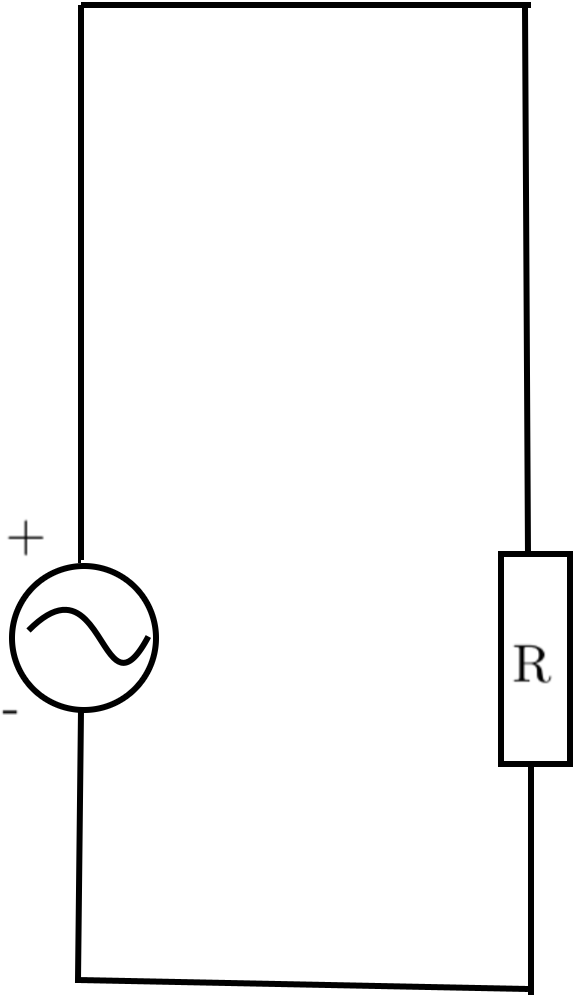
\includegraphics[width=30mm]{Imazhet/Qarku R.png}
		\caption{Qarku me Rezistencë (R).}
		\label{fig:boat1}
	\end{figure}
	
	$ \sim \Rightarrow $ Rryma alternative.
	
	$R \Rightarrow $ Rezistenca.
	
	\begin{center}
		Grafiku:
	\end{center}
	
	\begin{figure}[h]
		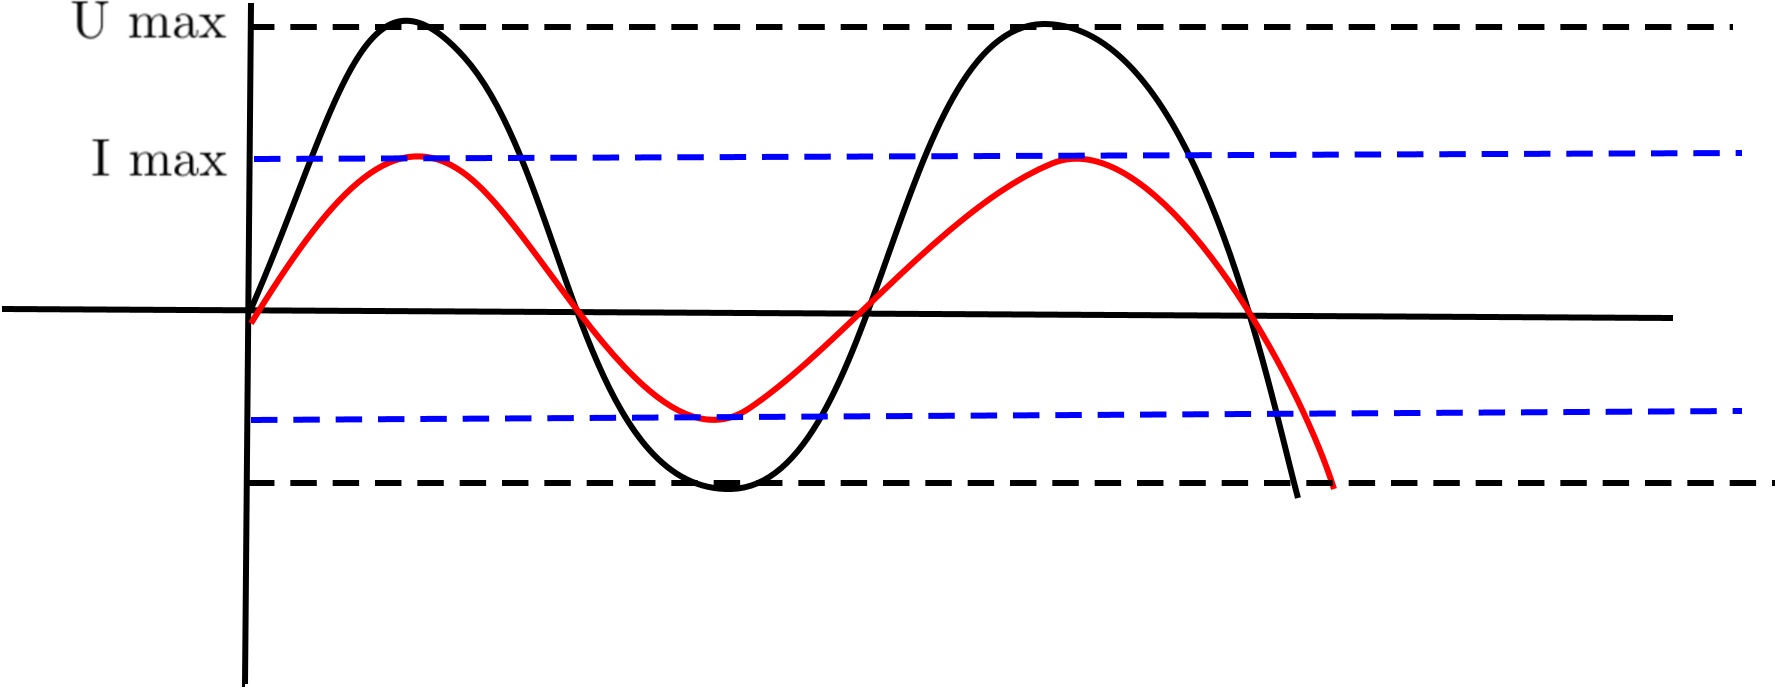
\includegraphics[width=70mm]{Imazhet/Grafik R.png}
		\caption{Grafiku i I  dhe U.}
		\label{fig:boat1}
	\end{figure}
	
	\begin{center}
		Vektorët:
	\end{center}
	\begin{figure}[h]
		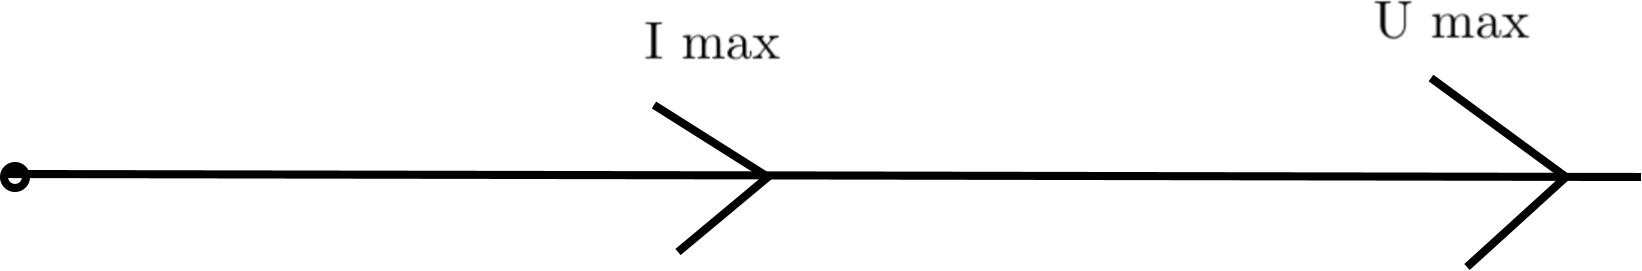
\includegraphics[width=70mm]{Imazhet/Vektor R.png}
		\caption{Ndërtimi vektorial i I dhe U(R) .}
		\label{fig:boat1}
	\end{figure}
	
	$I_{max}= \frac{U_{max}}{R}$
	
	$I_{ef}= \frac{U_{ef}}{R}$
	
	\begin{center}
		Ekuacionet:
	\end{center}
	
	$I_{(t)} = I_{max} \cdot sin (\omega\cdot t) \Rightarrow $ $I_{(t)} = I_{max} \cdot cos (\omega\cdot t- \pi)$
	
	
	$U_{(t)} = U_{max} \cdot sin (\omega\cdot t) \Rightarrow $ $U_{(t)} = U_{max} \cdot cos (\omega\cdot t- \pi)$\\
	
	\begin{center}
		Qarku me bobinë (L).
	\end{center}
	
	\begin{figure}[h]
		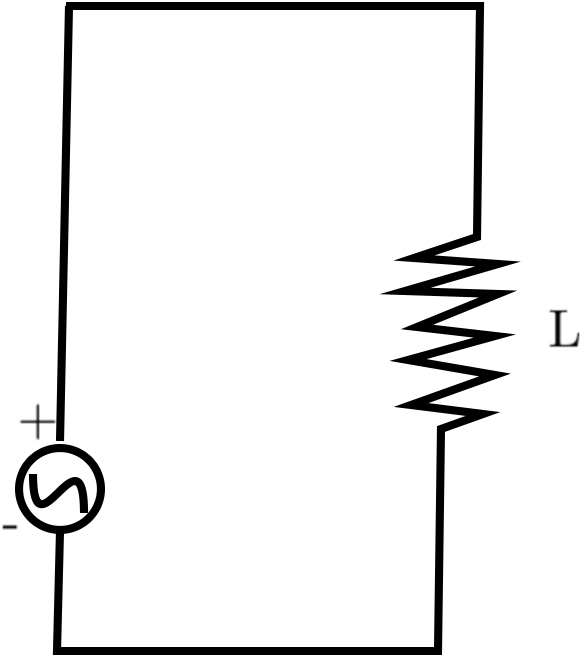
\includegraphics[width=30mm]{Imazhet/Qarku L.png}
		\caption{Qarku me bobinë (L) .}
		\label{fig:boat1}
	\end{figure}
	
	
	
	
	$ \sim \Rightarrow $ Rryma alternative.
	
	$L \Rightarrow $ Bobina.
	
	\begin{center}
		Grafiku:
	\end{center}
	
	\begin{figure}[h]
		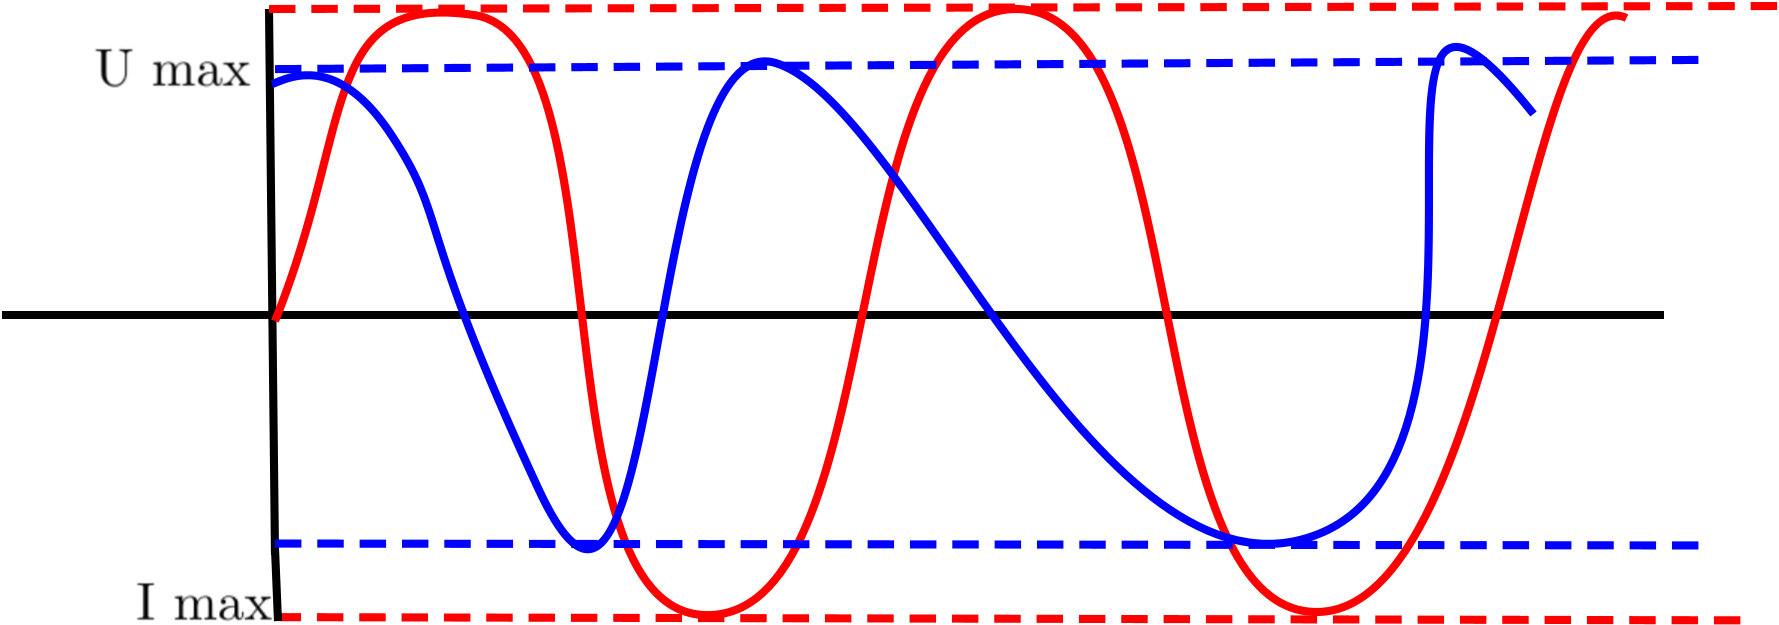
\includegraphics[width=70mm]{Imazhet/Grafik L.png}
		\caption{Grafiku i I  dhe U.}
		\label{fig:boat1}
	\end{figure}
	\begin{center}
		Vektorët:
	\end{center}
	\begin{figure}[h]
		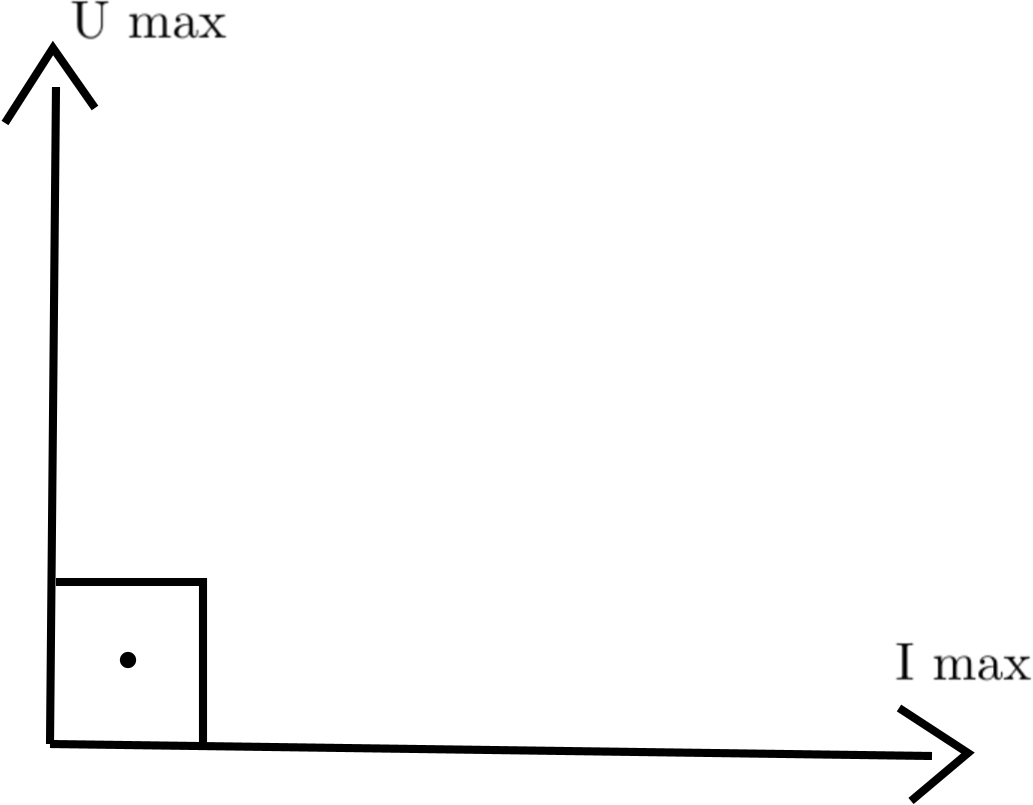
\includegraphics[width=40mm]{Imazhet/Vektor L.png}
		\caption{Ndërtimi vektorial i I  dhe U(L).}
		\label{fig:boat1}
	\end{figure}
	
	\begin{center}
		Ekuacionet:
	\end{center}
	
	$U_{(t)}= U_{max} \cdot cos (\omega\cdot t)$
	
	
	$I_{(t)}= I_{max} \cdot sin (\omega\cdot t) \Rightarrow I_{(t)}= I_{max} \cdot cos(\omega \cdot t - \frac{\pi}{2})$\\
	
	
	
	
	\textit{"Përshkak të forcës elektromotore të induksionit,indesiteti i rrymës(I) nuk i arrinë vlerat e tij maksimale në ato çaste kur tensioni(U) i tij është maksimal,rryma(I) arrinë vlerën maksimale kur forca elektromotore është 0.Pra rryma(I) është me $\varphi_0$(Vonesë  faze) $\frac{\pi}{2}$ nga U(Tensioni)."}\\
	
	
	
	\begin{center}
		Qarku me kondesatorë (C).
	\end{center}
	
	\begin{figure}[h]
		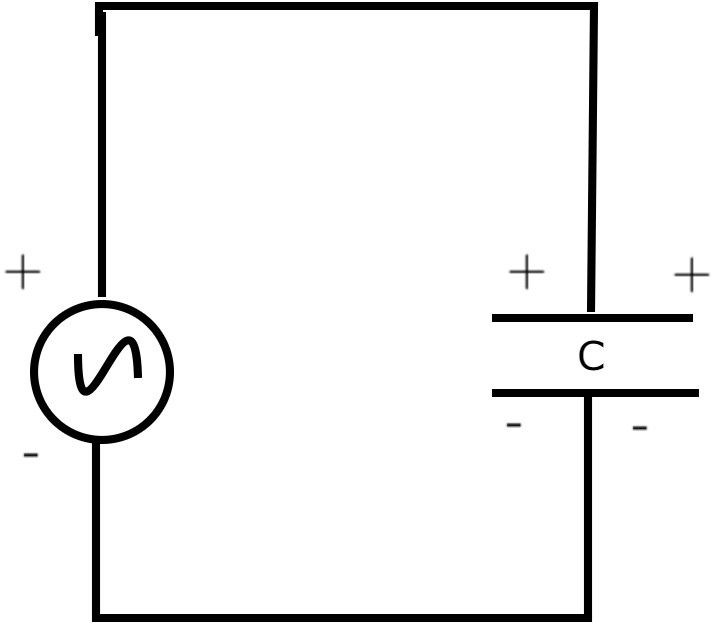
\includegraphics[width=50mm]{Imazhet/Qarku C.jpg}
		\caption{Qarku me kondesatorë (C).}
		\label{fig:boat1}
	\end{figure}
	$ \sim \Rightarrow $ Rryma alternative.
	
	
	$C \Rightarrow $ Kondesatori.
	
	\begin{center}
		Grafiku:
	\end{center}
	\begin{figure}[h]
		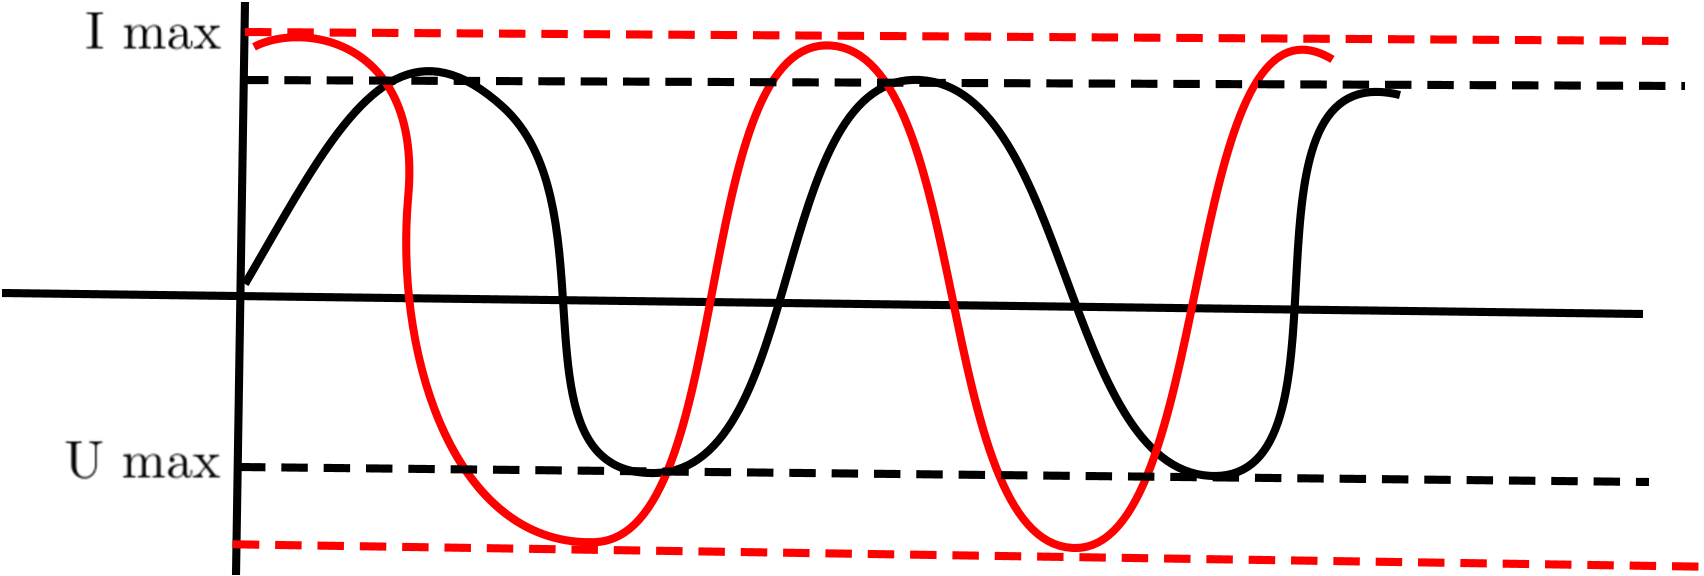
\includegraphics[width=70mm]{Imazhet/Grafik C.png}
		\caption{Qarku me kondesatorë (C).}
		\label{fig:boat1}
	\end{figure}
	
	\begin{center}
		Ekuacionet:
	\end{center}
	
	$I_{(t)}= I_{max} \cdot sin (\omega \cdot t)$\\
	
	
	$U_{(t)}= U_{max} \cdot cos (\omega \cdot t)$ $\Rightarrow$ $U_{(t)}= U_{max} \cdot sin (\omega \cdot t - \frac{\pi}{2})$
	
	\begin{center}
		Vektorët:
	\end{center}
	
	\begin{figure}[h]
		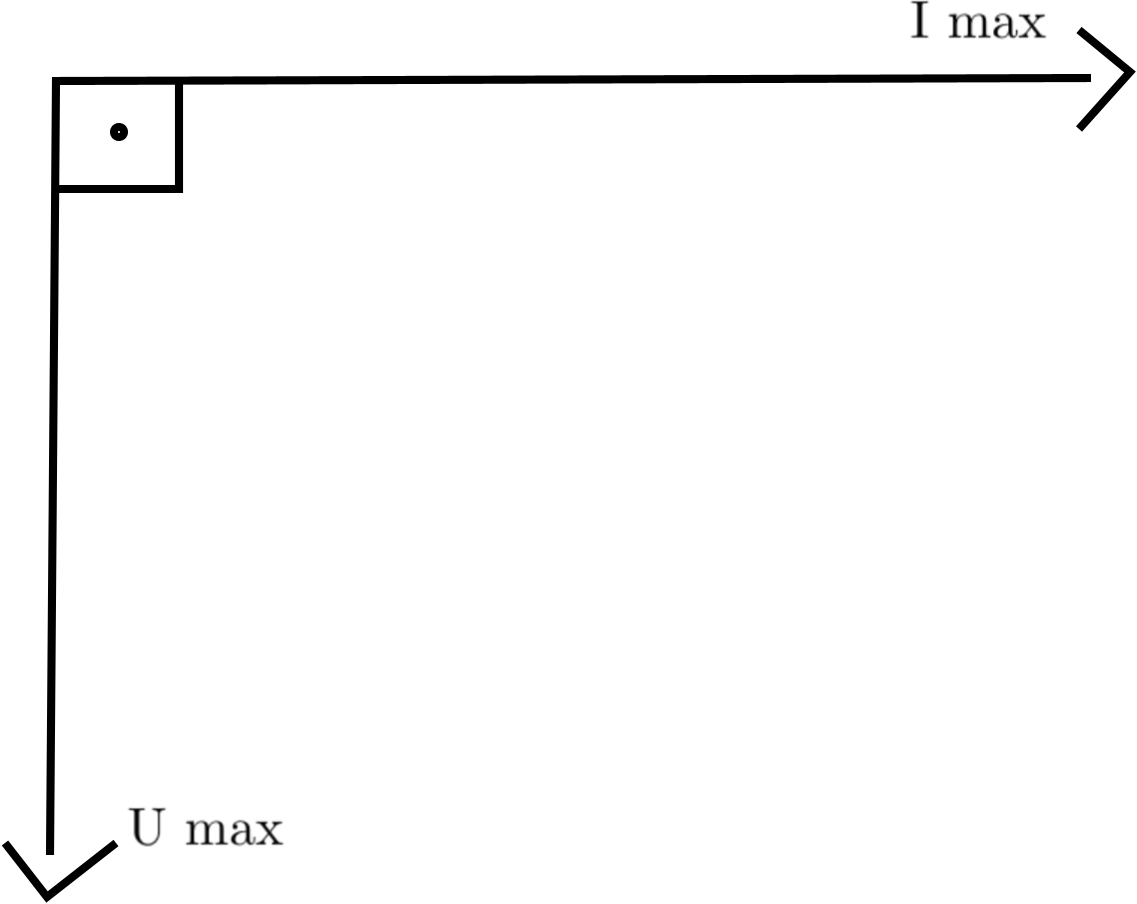
\includegraphics[width=40mm]{Imazhet/Vektor C.png}
		\caption{Ndërtimi vektorial i I  dhe U(C).}
		\label{fig:boat1}
	\end{figure}
	
	\begin{center}
		Rezistencat induktive.
	\end{center}
	
	$X_{L} \Rightarrow $ Rezistenca induktive e bobinës. $X_{L}=\omega \cdot L$\\
	
	
	
	$X_{C} \Rightarrow $ Rezistenca induktive e kondesatorit.
	
	$X_{C}=\frac{1}{\omega \cdot C}$\\
	
	
	\begin{center}
		Qarku R,L,C.
	\end{center}
	\begin{figure}[h]
		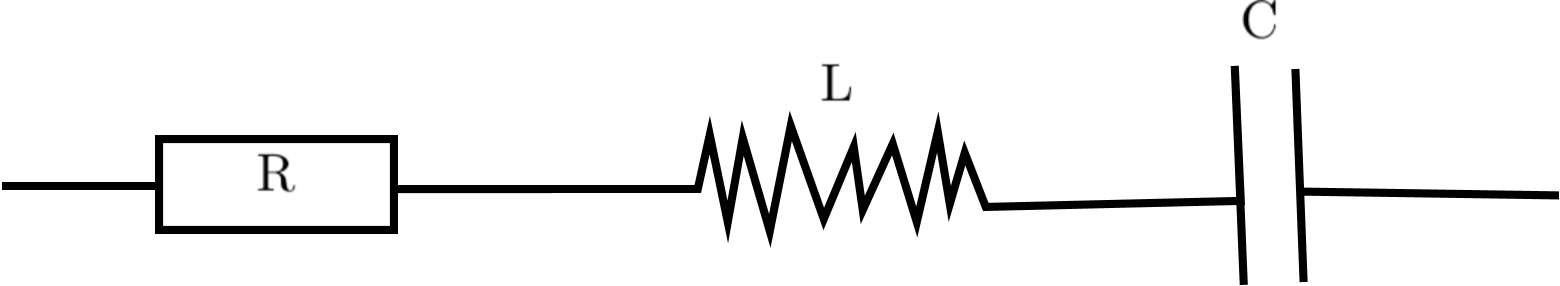
\includegraphics[width=70mm]{Imazhet/Qarku R,L,C.png}
		\caption{	Qarku R(Rezistenca),L(Bobina),C(Kondesatori).}
		\label{fig:boat1}
	\end{figure}
	
	
	$Z \Rightarrow $ Rezistenca e përgjithshme.\\
	
	
	$Z= \sqrt{R^2+(X_L - X_C)^2}$
	
	\section{Valët.}
	
	\begin{center}
		\textit{Simbolet:}
	\end{center}
	
	$\lambda \Rightarrow $ Gjatësia e valës.(m)
	
	$T \Rightarrow $ Perioda.
	
	$f \Rightarrow$ Frekuenca.
	
	$v$ ose $c$ $\Rightarrow$ Shpejtësia.
	
	$A \Rightarrow$ Amplituda.
	

	
	\begin{center}
		Formula:
	\end{center}
	
	$v=\frac{\lambda}{T}= \lambda \cdot f$
	
	$T= \frac{1}{f}$
	
	$f=\frac{1}{T}$
	
	$\lambda = v \cdot T$
	\begin{figure}[h]
		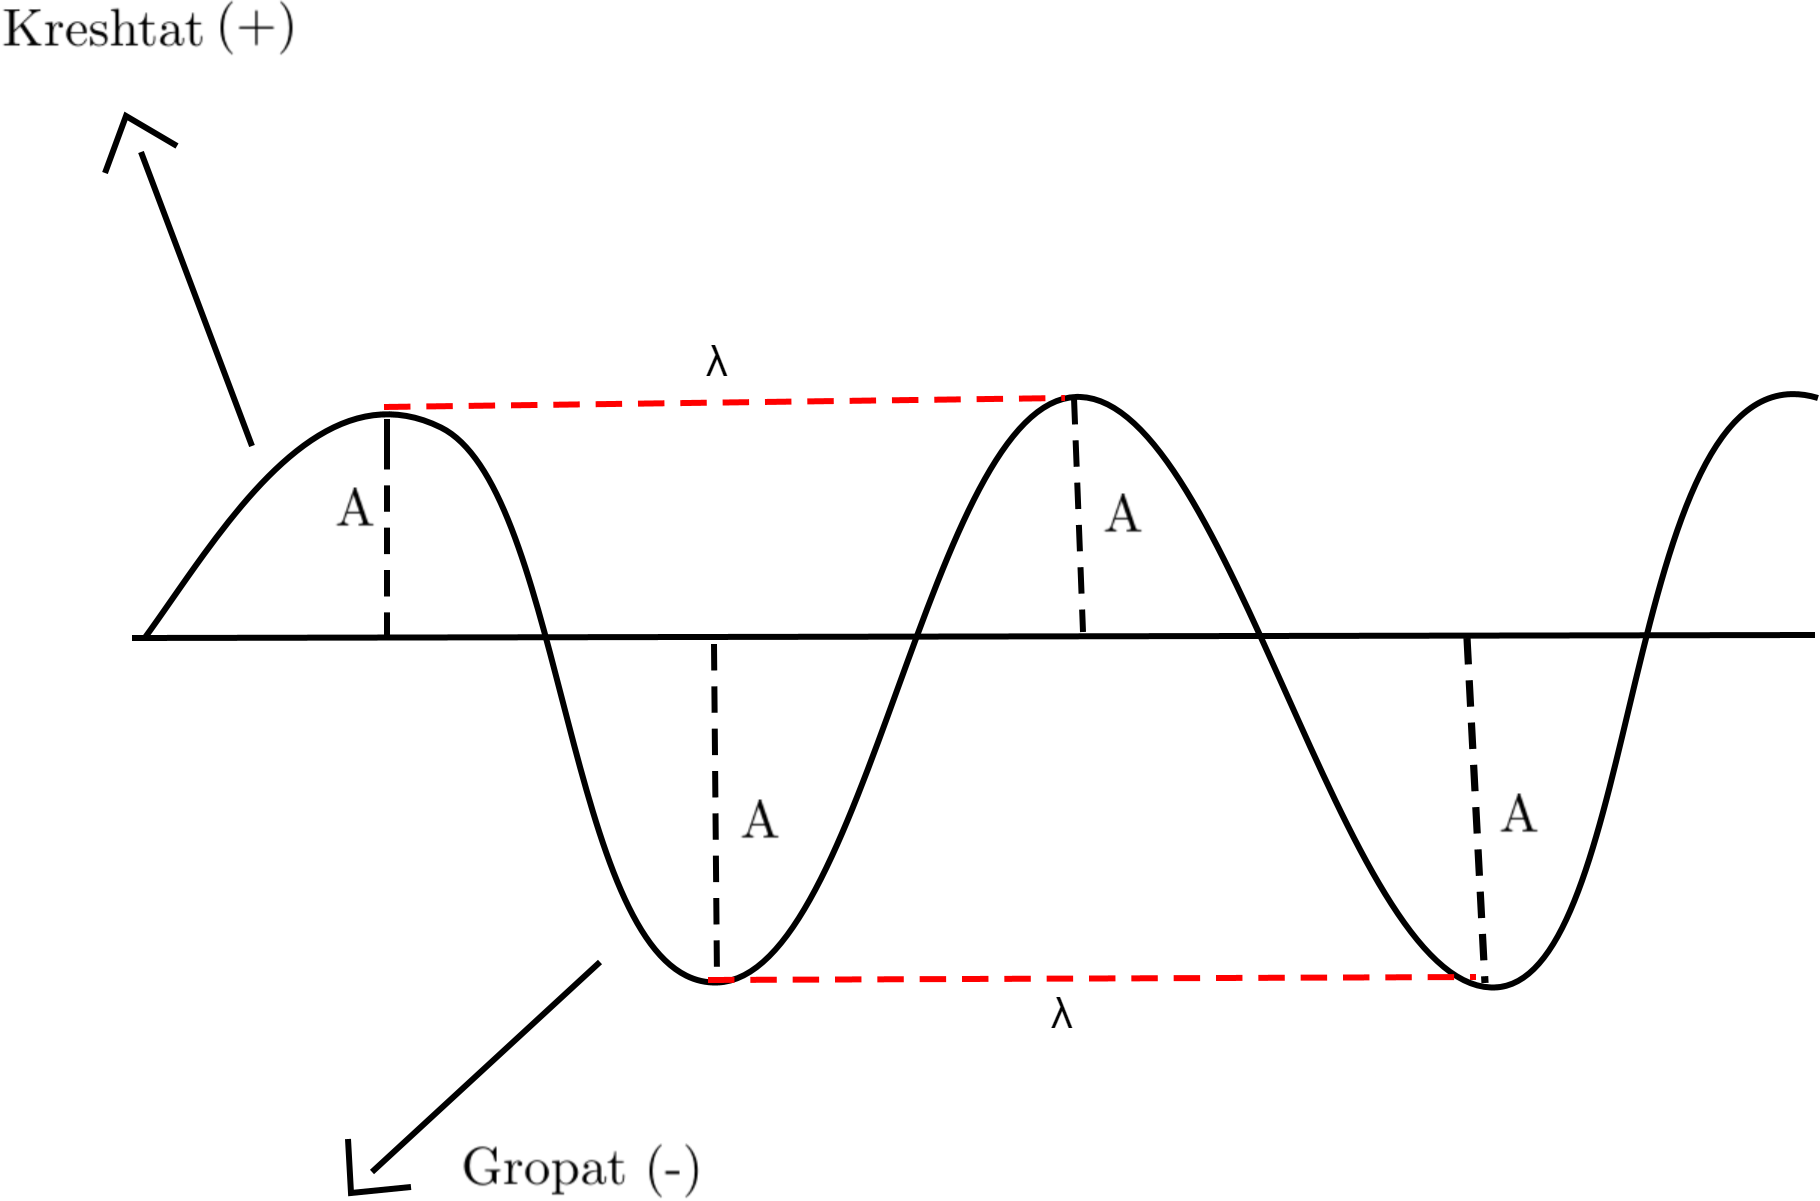
\includegraphics[width=70mm]{Imazhet/valet.png}
		\caption{Valët e vizatura në një grafik me $A$ me $\lambda$.}
		\label{fig:boat1}
	\end{figure}
	
	\textbf{16.1 Valët elastike.}
	
	\begin{figure}[h]
		\includegraphics[width=70mm]{Imazhet/vale elastike.png}
		\caption{Lëkundja e pikave tregon që lëvizja elastike e valëve nuk zhvendos asnjë pikë por atyre i ndryshon $A$.}
		\label{fig:boat1}
	\end{figure}
	
	\begin{center}
		\textit{"Vala nuk transporton lënd."}
	\end{center}
	
	
	\textbf{Ekuacioni i valës.}
	
	$x= A \cdot sin [\frac{2 \pi}{T} \cdot (t -\frac{x}{v})]$\\
	
	
	
	\begin{center}
		Parimi i Hygensit.
	\end{center}
	\begin{figure}[h]
		\includegraphics[width=60mm]{Imazhet/Parimi i Hygensit.png}
		\caption{Parimi i Hygensit për valët.}
		\label{fig:boat1}
	\end{figure}
	
	Çdo pikë e sipërfaqes së valës,shërben si burim
	pikësor valësh.
	
	\textbf{2 Pohimet e parimit të Hygensit.}
	
	\textbf{1.}Nëse $S_1$ është sipërfaqe vale atëherë dhe mbështjellsja $S_2$ e valëve elementare të lëshuara një kohësishtë nga pikat $S_1$, është sipërfaqe vale.
	
	
	$S1$ dhe $S_2$ $\Rightarrow$ Janë sipërfaqe vale.
	
	\textbf{2. }Drejtimet e përhapjes së valës(rrezet) janë
	drejtezat që bashkojnë burimet elementare me pikat
	, ku mbështjellsja takon valët elementare.\\
	
	
	
	\textbf{16.2 Mbivendosja e valëve.}
	
		\begin{figure}[h]
		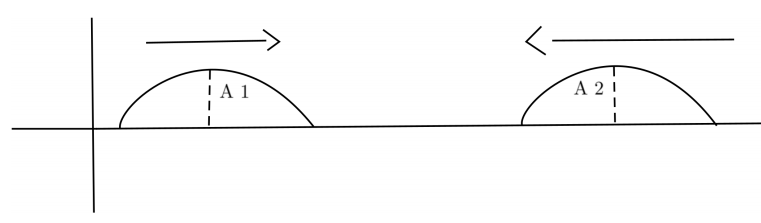
\includegraphics[width=80mm]{Imazhet/mbivendosja1.png}
		\caption{ Dy valë që kan drejtim të njëjtë.}
		\label{fig:boat1}
	\end{figure}

Në këtë rast valët kan fazë fillestare $\varphi_0=0$.


Pasi valët takohen ato mbivendosen me njëra-tjetrën.\\
	
\textbf{	Pasi bashkohen:}

	\begin{figure}[h]
	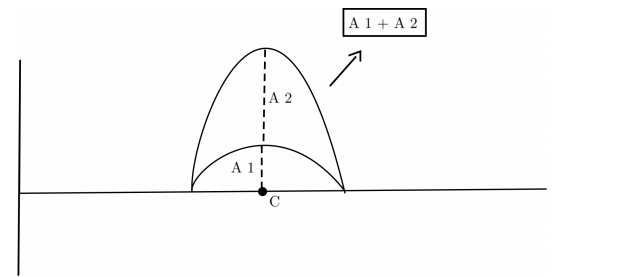
\includegraphics[width=80mm]{Imazhet/mbivendosja2.png}
	\caption{ Dy valë pasi janë godituar me njëra-tjetrën
		në një pikë $C$.}
	\label{fig:boat1}
\end{figure}

\textbf{Pasi kalojnë njëra-tjetrën:}
	
		\begin{figure}[h]
		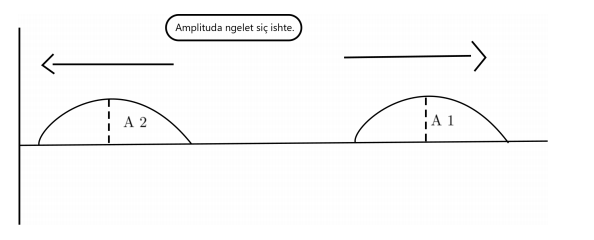
\includegraphics[width=80mm]{Imazhet/mbivendosja3.png}
		\caption{ Dy valë pasi janë larguar nga njëra-tjetra.}
		\label{fig:boat1}
	\end{figure}

Efektet e dy valëve që arrijnë njëkohësisht në një
pikë, mjediset e tyre  mblidhen.Përhapja e secilës valë bëhet
sikur të mos kishte takuar në rrugën e saj valën tjetër.
\\


\textbf{16.2.1 Dy valë në anë të kundërta:}

	\begin{figure}[h]
	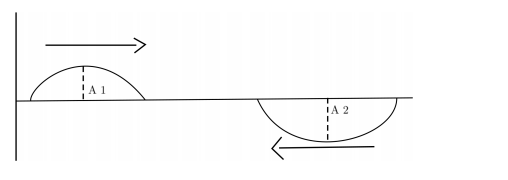
\includegraphics[width=80mm]{Imazhet/mbivendosja4.png}
	\caption{ Dy valë që kan drejtim të njëjtë.}
	\label{fig:boat1}
\end{figure}

Në këtë rast valët kan fazë fillestare $\varphi_0=0$.


\textbf{Pasi bashkohen:}

Dy valët zbriten nga më e madhja tek më
e vogla dhe ngelet rezultatija.

	\begin{figure}[h]
	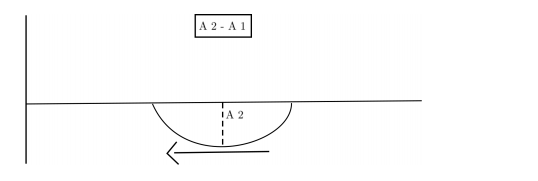
\includegraphics[width=80mm]{Imazhet/mbivendosja5.png}
	\caption{ Dy valët të cilat janë bashkuar.}
	\label{fig:boat1}
\end{figure}

\textbf{16.3 Interferenca.}

Dukuria e mbivendosjes së valëve harmonike me
frekuencë të njëjtë quhet interferenc.Burimi që shkaktojnë këto valë quhen koherente.(Diferenca e fazave
nuk ndryshon me kohën.)

\begin{center}
	\textit{Simbolet:}
\end{center}

$A \Rightarrow $ Amplituda.

$x$ $\Rightarrow$ Gjatësia.

$k \Rightarrow $ Numri i gjatësis së valës.

$\lambda  \Rightarrow$ Gjatësia e valës.

$\Delta \lambda  \Rightarrow $ Gjatësia e përgjithshme.

\begin{center}
	Formula:
\end{center}

$Max.A_1 + A2$
$\Delta x = x_1 + x_2 = k \cdot \lambda$

$\Delta x = x_1 + x_2 = k \cdot \frac{\lambda}{2}$\\

$Min.A_1 - A_2$

$\Delta x = x_1 + x_2 = (2k + 1) \cdot \lambda$\\

\textbf{16.4 Valët e qendrueshme.}

	\begin{figure}[h]
	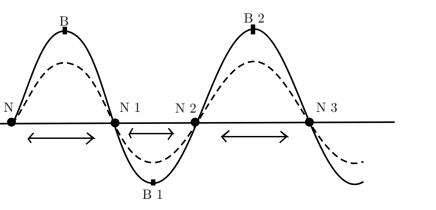
\includegraphics[width=70mm]{Imazhet/Valet e qendrueshme.png}
	\caption{Valët e qendrueshme të skicuara.}
	\label{fig:boat1}
\end{figure}

$N_1,N_2,N_3,N_4,N_5,N_6 \Rightarrow $ janë nyje të valës dhe nuk lëkunden.


$B_1,B_2,B_3,B_4,B_5,B_6 \Rightarrow$  gropat dhe kreshtat lëvizin pozicionet.


 $\bullet$  \textbf{ Kordat e fiksuara në dy pika:}
	\begin{figure}[h]
	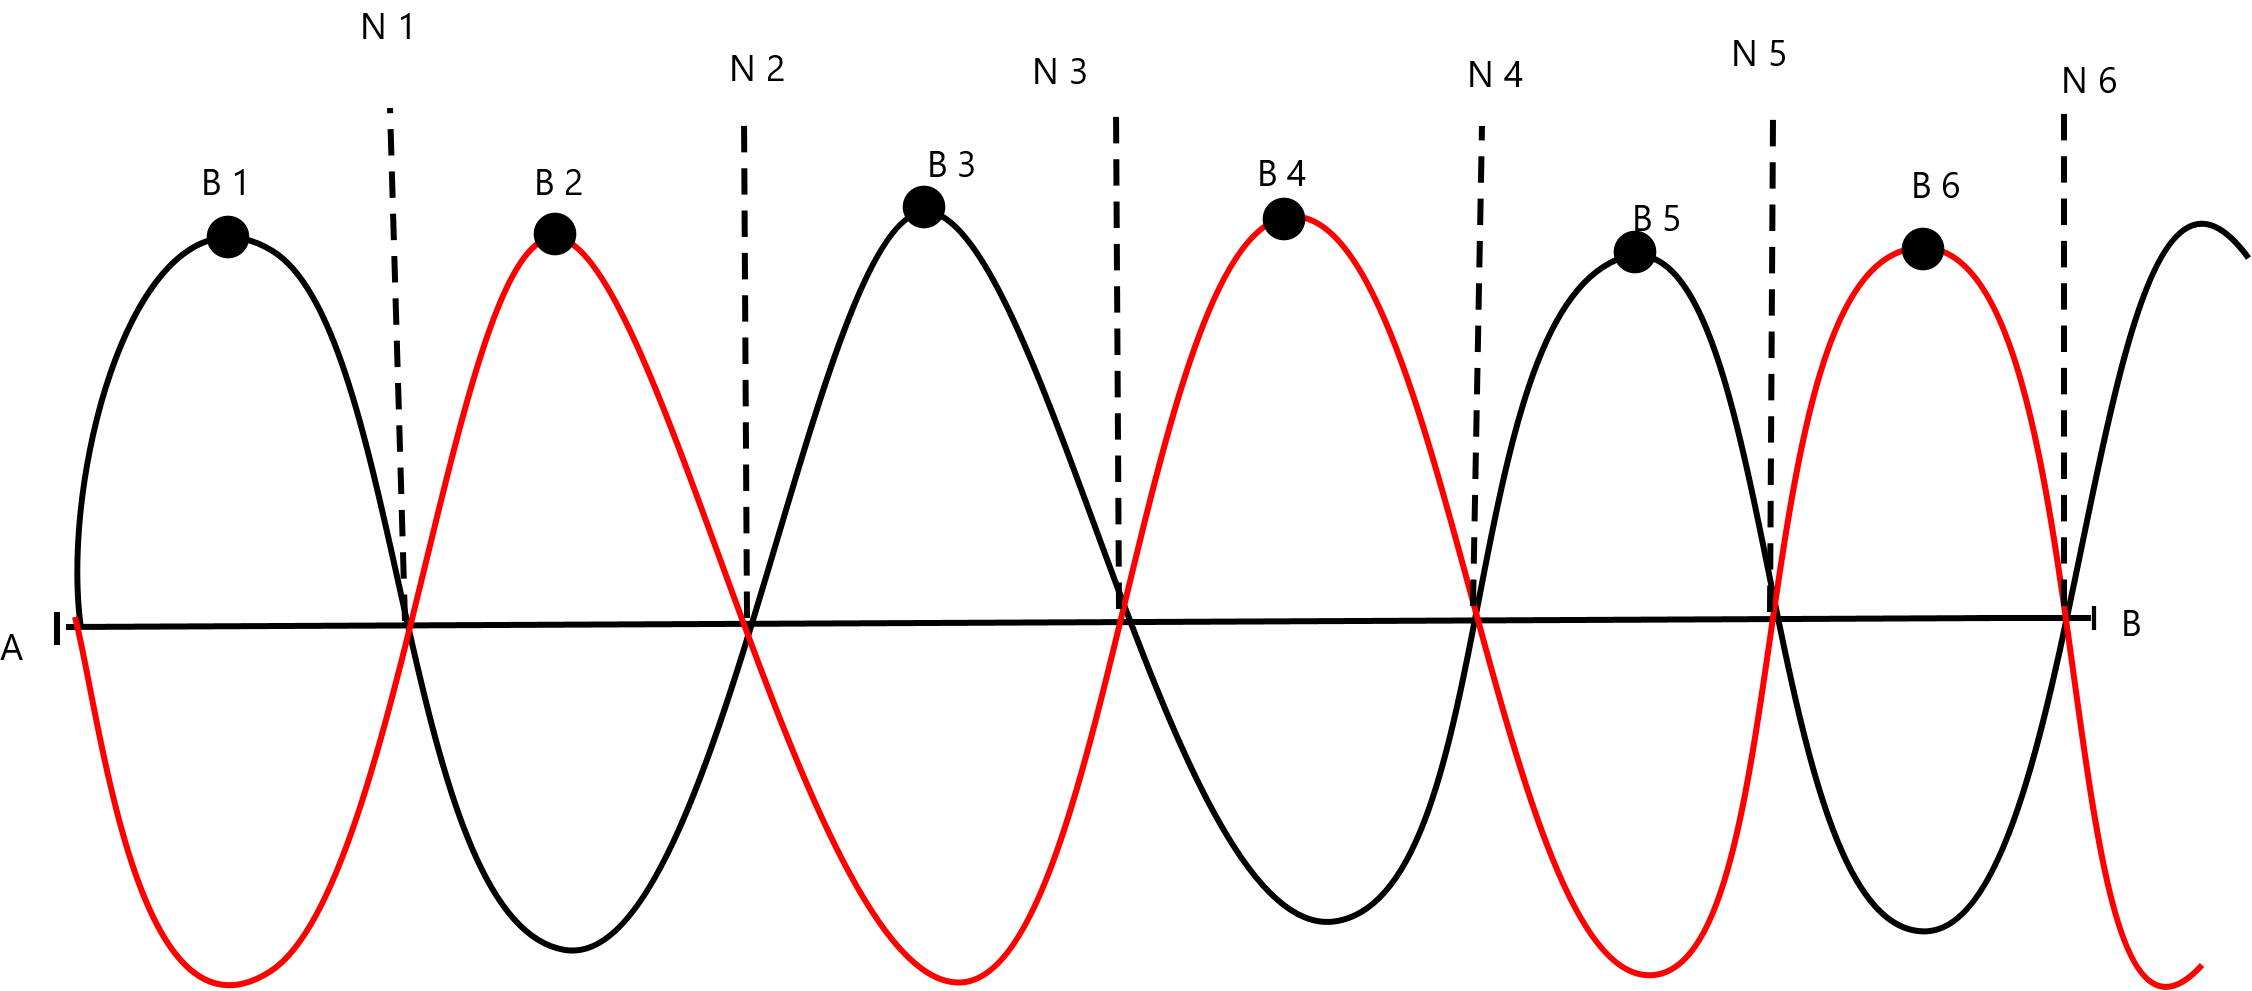
\includegraphics[width=70mm]{Imazhet/Valet e qendrueshme1.png}
	\caption{Valët e qendrueshme të skicuara.}
	\label{fig:boat1}
\end{figure}

Në rastin kur korda është e fiksuar në të dyja anët valët e qendrueshme vendosen nëse gjatësia e saj është një numër i plotë ngjysëm gjatësie vale.

$l= n \cdot \frac{\lambda}{2}$\\


 $\bullet$  \textbf{ Kordat e fiksuara në një pikë:}
 
	\begin{figure}[h]
	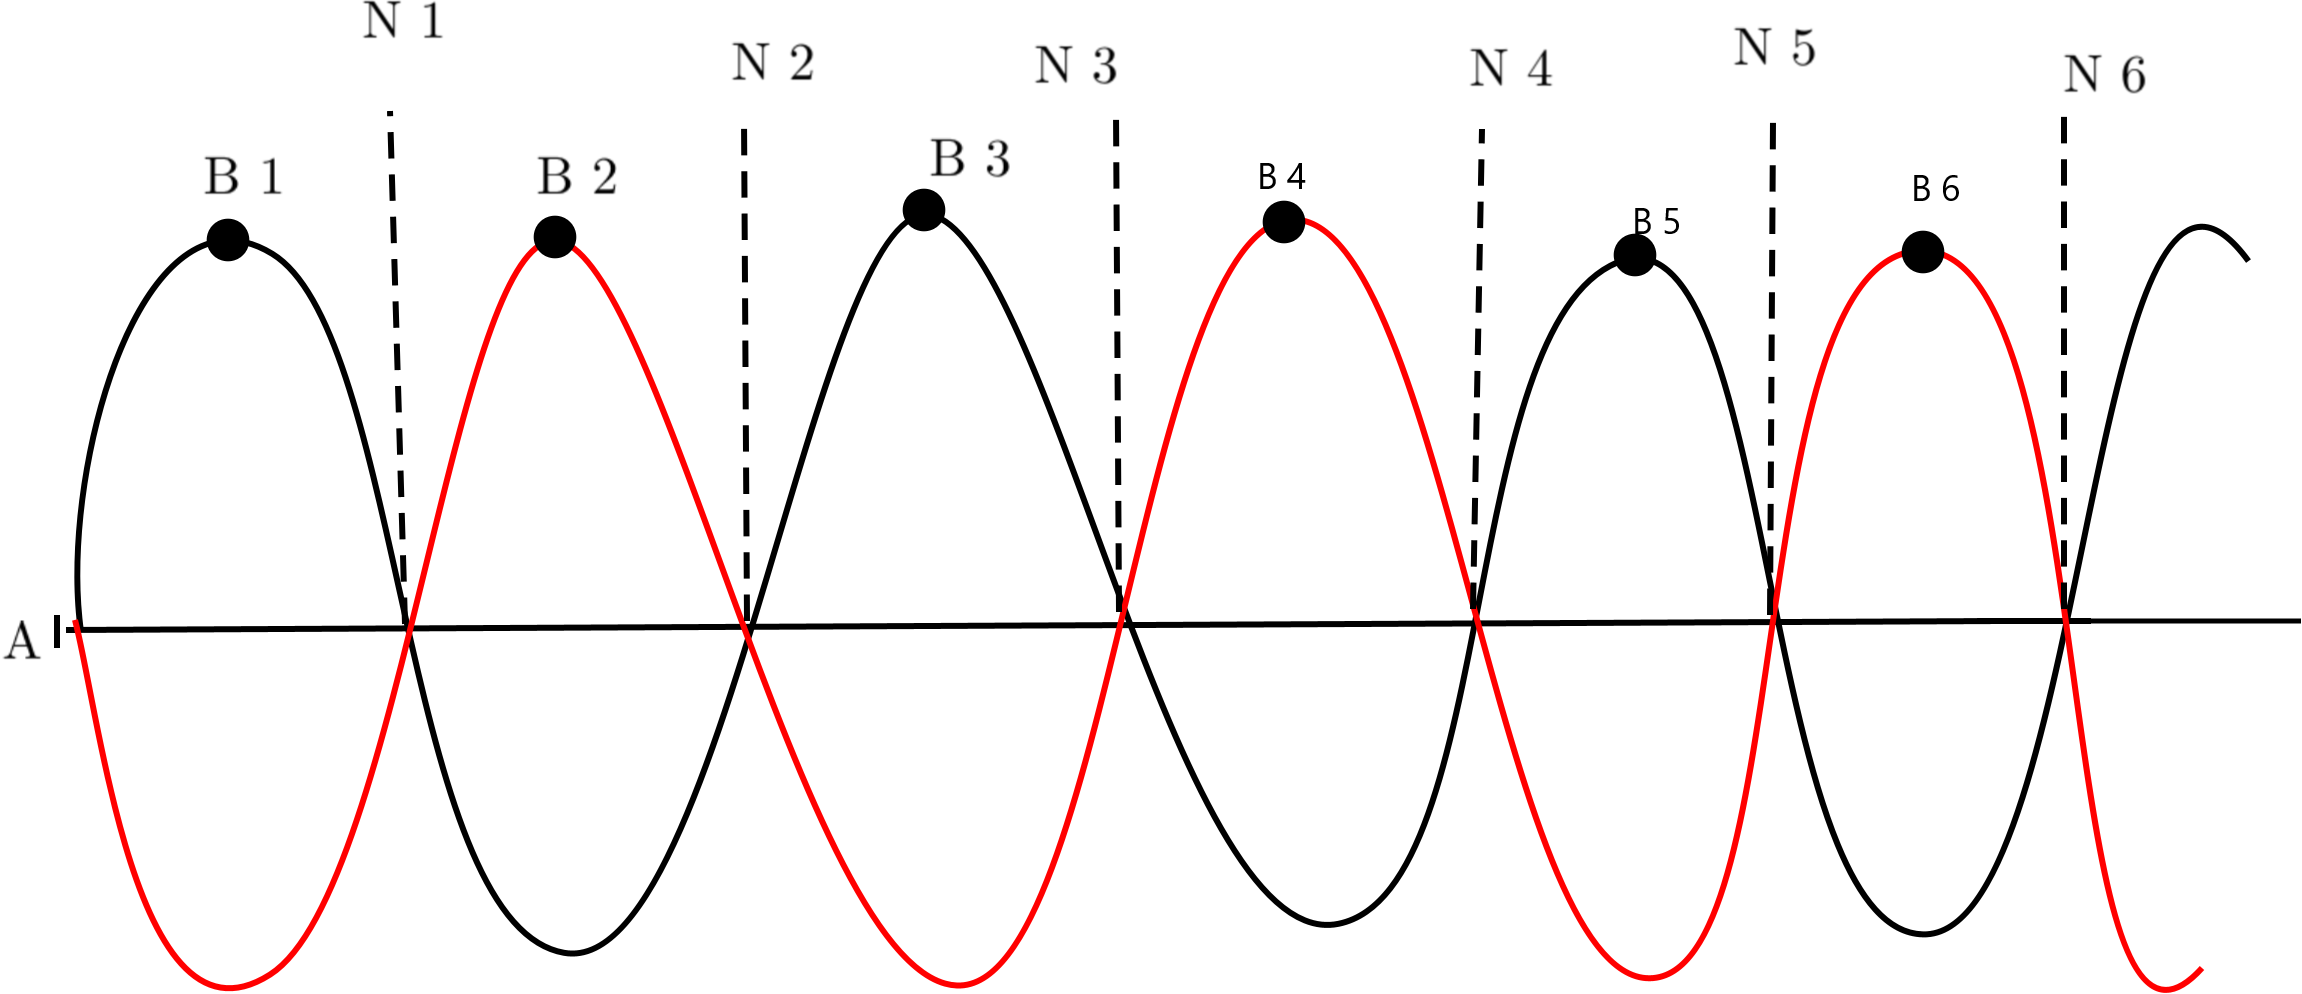
\includegraphics[width=70mm]{Imazhet/Valet e qendrueshme2.png}
	\caption{Valët e qendrueshme të skicuara.}
	\label{fig:boat1}
\end{figure}

Në rastin kur korda është e fiksuar në një anë duhet që gjatësia e kordës të jet tek dhe një numër çerek gjatësie vale.

$l=(2n+1)\cdot \frac{\lambda}{4}$\\


\textbf{16.5 Frekuenca e lëkundjes së kordave.}

\begin{center}
	\textit{Simbolet:}
\end{center}

$n$$\Rightarrow$ Numri i pjesëve të ndara në kordë.

$f\Rightarrow $ Frekuenca.($H_z$)

$v \Rightarrow$ Shpejtësia$(m/s)$

$l \Rightarrow $ Gjatësia e kordës.



\begin{center}
	Formula:
\end{center}

$f= n \cdot \frac{v}{2\cdot l}$ Formula e përgjithshme.\\




 $\bullet$  \textbf{ Kur korda ndahet në dy pjesë:}
 
 $f=\frac{1}{2} \cdot \frac{v}{2 \cdot l}$\\
 
  $\bullet$  \textbf{ Kur korda ndahet në tre pjesë:}
  
   $f=\frac{1}{3} \cdot \frac{v}{2 \cdot l}$\\
   
     $\bullet$  \textbf{ Kur korda ndahet në katër pjesë:}
 
    $f=\frac{1}{4} \cdot \frac{v}{2 \cdot l}$\\
    
    
         $\bullet$  \textbf{ Kur korda ndahet në gjashtë pjesë:}
    
     $f=\frac{1}{6} \cdot \frac{v}{2 \cdot l}$\\

\textbf{16.6 Valët zanore.}

	\begin{figure}[h]
	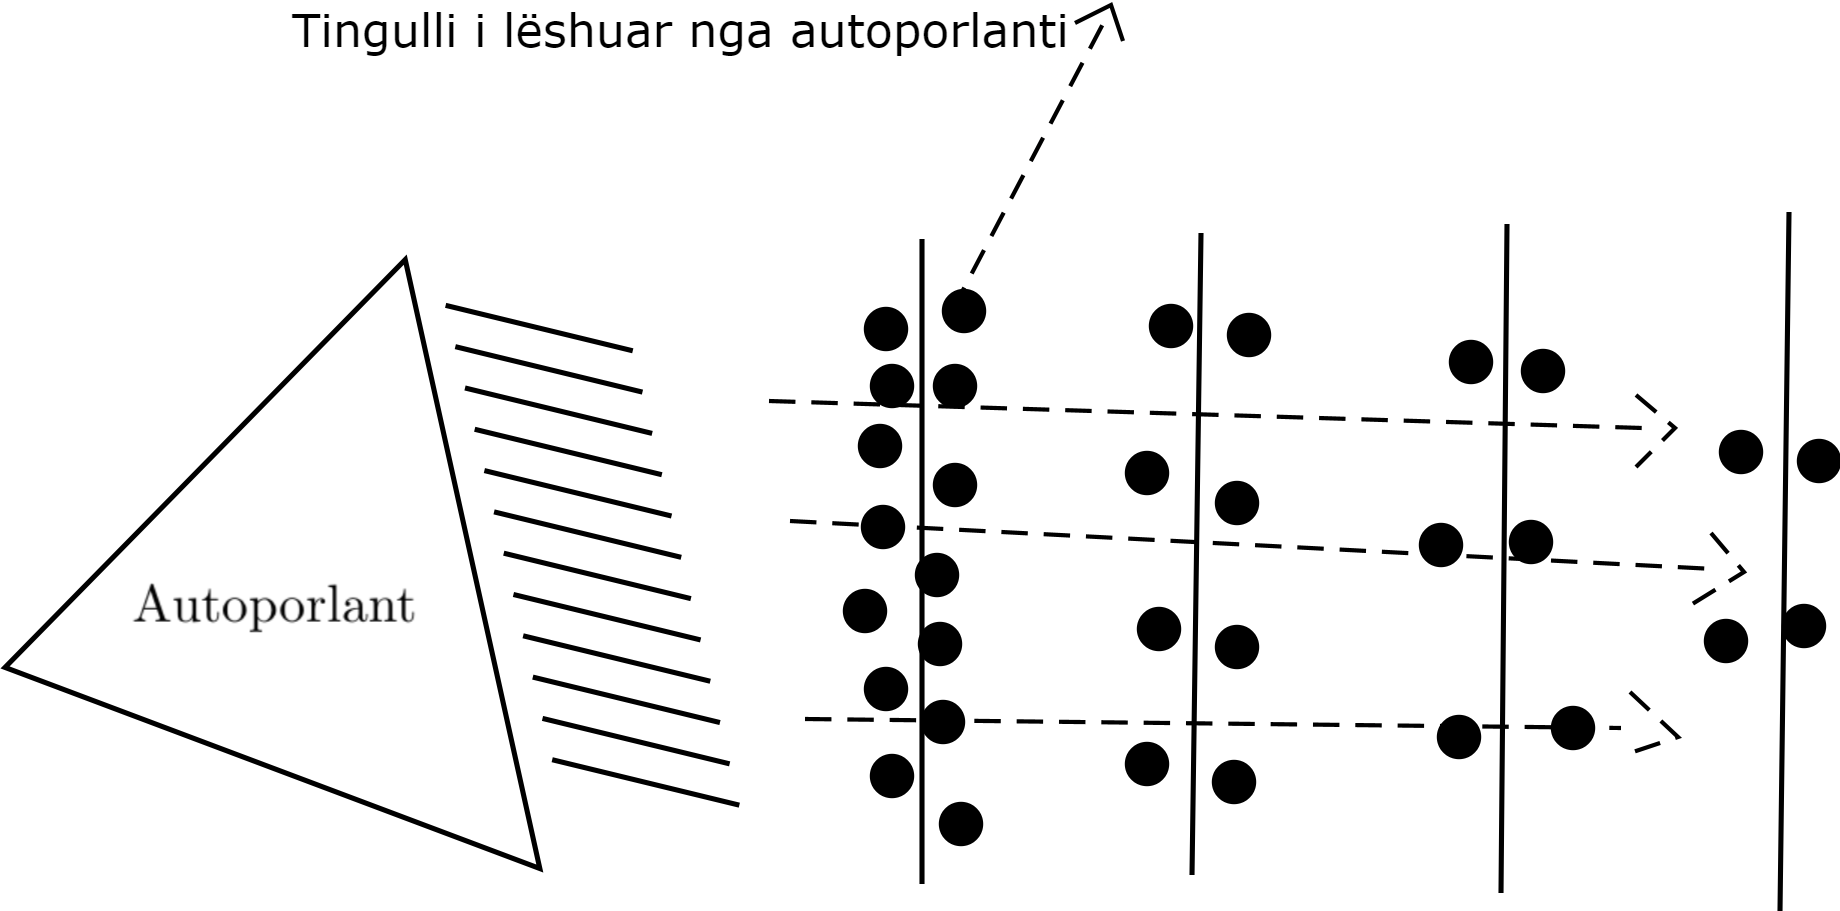
\includegraphics[width=80mm]{Imazhet/Valetzanore.png}
	\caption{Valët e lëshuara nga një autoporlant.}
	\label{fig:boat1}
\end{figure}

$<20 H_Z \Rightarrow $ Infra tinguj.

$>20,000 H_Z \Rightarrow $ Ultra tinguj.

\begin{center}
	\textit{Simbolet:}
\end{center}

$v \Rightarrow$ Shpejtësia .$(m/s)$

$T \Rightarrow $ Temperatura.

	$I_v \Rightarrow $ Intesiteti i valës.
	
	$E \Rightarrow $ Energjia.
	
	$S \Rightarrow$ Sipërfaqa.
	
	$t \Rightarrow$ Koha.

\begin{center}
	Formula:
\end{center}

$v=331,6 (1+0,002 \cdot T)$

$I_v=\frac{E}{S \cdot t}$\\

\textbf{16.7 Valët rrethore.}

Ndodhin kur pikat e mjedist lëkunden pingule($\perp$) me vijat e përhapjes.\\

\textbf{16.8 Valët gjatësore.}

Ndodhin atëherë kur lëkundja e pikave bëhet në drejtimin e përhapjes së valës.\\


\textbf{16.9 Efekti Dopler.}

	\begin{figure}[h]
	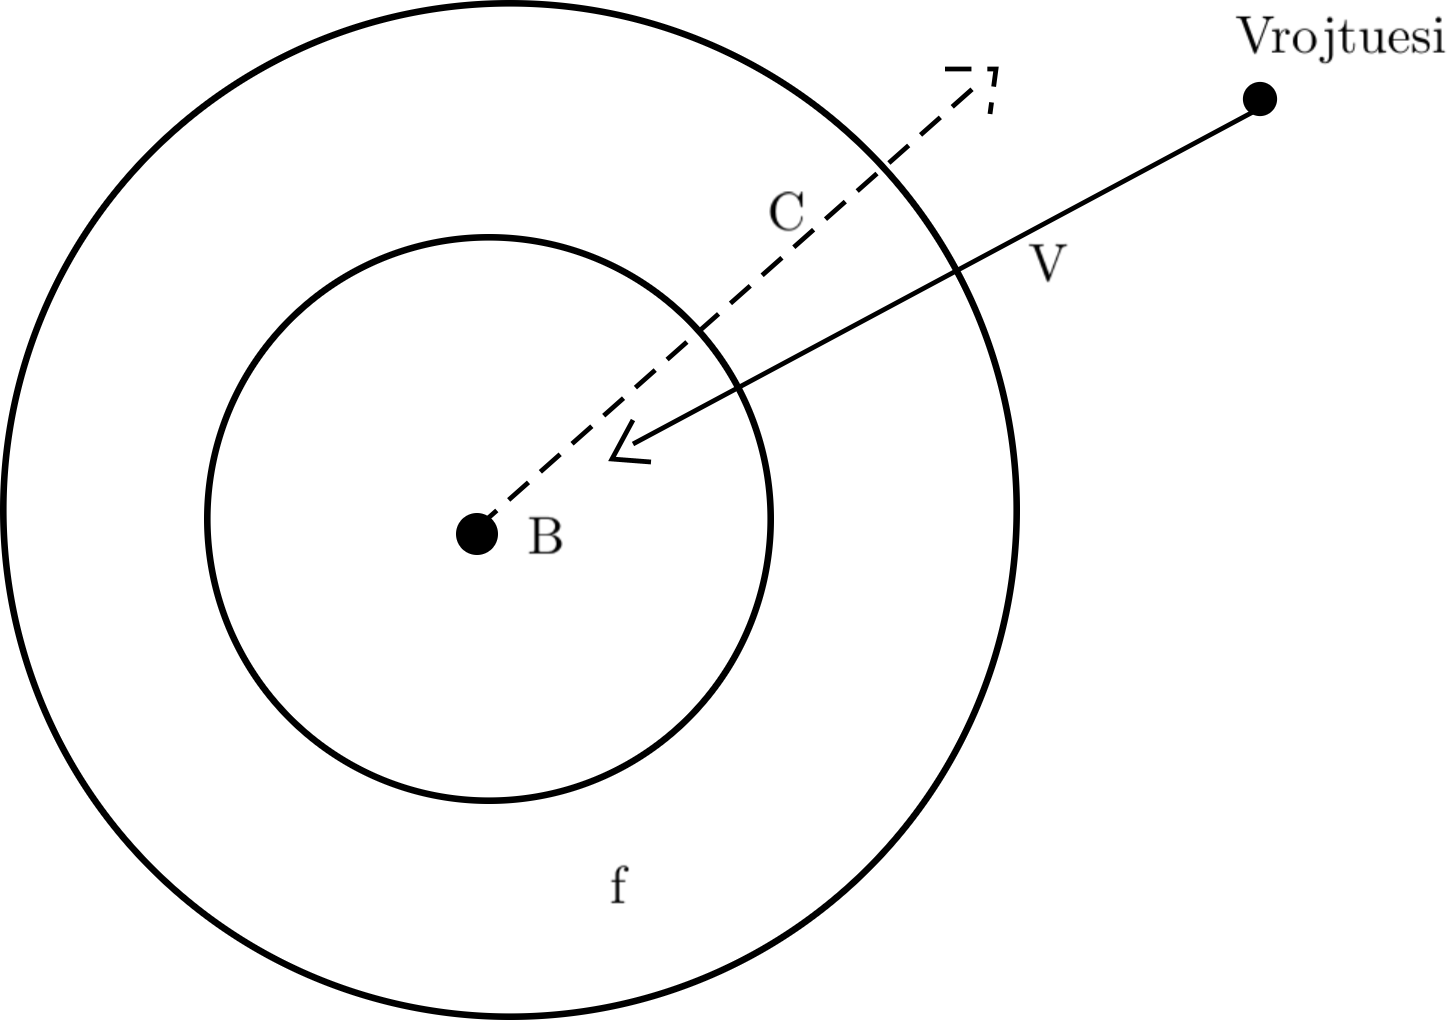
\includegraphics[width=70mm]{Imazhet/efekti dopler.png}
	\caption{Efekti Dopler.}
	\label{fig:boat1}
\end{figure}

\begin{center}
\textit{	Simbolet:}
\end{center}

$\vec{v} \Rightarrow $ Shpejtësia e vrojtesit.

$\vec{c}$ ose $ v_0 $ $ \Rightarrow $ Shpejtësia e përhapjes së tingullit.

$B \Rightarrow$ Burimi i tingullit.

$f \Rightarrow $ Frekuenca e burimit.

$f_v \Rightarrow $ Frekuenca që dëgjon vrojtuesi.

$\lambda \Rightarrow$ Gjatësia e valës.

$c' \Rightarrow $ Shpejtësia e vrojtuesit dhe ajo e burimit kur mblidhen.


\begin{center}
	Formula:
\end{center}

$f=\frac{c'}{\lambda}= \frac{c+v}{\lambda}$\\

$f= f_v \cdot (\frac{c \pm v}{c \pm v_0} )$\\

$f= f_v \cdot (\frac{c + v}{c - v_0} )$ Kur kemi afrim.\\

$f= f_v \cdot (\frac{c - v}{c + v_0} )$ Kur kemi largim.\\


\textbf{16.10 Energjia.}

$\bullet$ \textbf{Përkufizim:}

Në amplitude ka energji potenciale.

Ne ekuilibër ka energji kinetike.

\begin{center}
	\textit{Simbolet:}
\end{center}

$E_m \Rightarrow$ Energjia mekanike.

$m \Rightarrow $ Masa.

$v \Rightarrow$ Shpejtësia.

$k \Rightarrow$ Koefiçent fërkimi.

$x \Rightarrow$ Gjatësia.

\begin{center}
	Formula:
\end{center}

$E_m=\frac{m \cdot v^2}{2}+ \frac{k \cdot x^2}{2}$

$= \frac{m  \cdot \omega^2 \cdot A^2 \cdot sin^2 \omega t }{2} + \frac{k \cdot A^2 \cdot sin^2 \omega t}{2}$

$= \frac{1}{2}\cdot k \cdot A^2$

$=\frac{k \cdot x^2}{2}$\\

 $*$ $E_m=\frac{k \cdot x^2}{2}$


$*$ $A=\sqrt{\frac{2E_m}{k}}$


\section{Pasqyrimi.}


	\begin{figure}[h]
	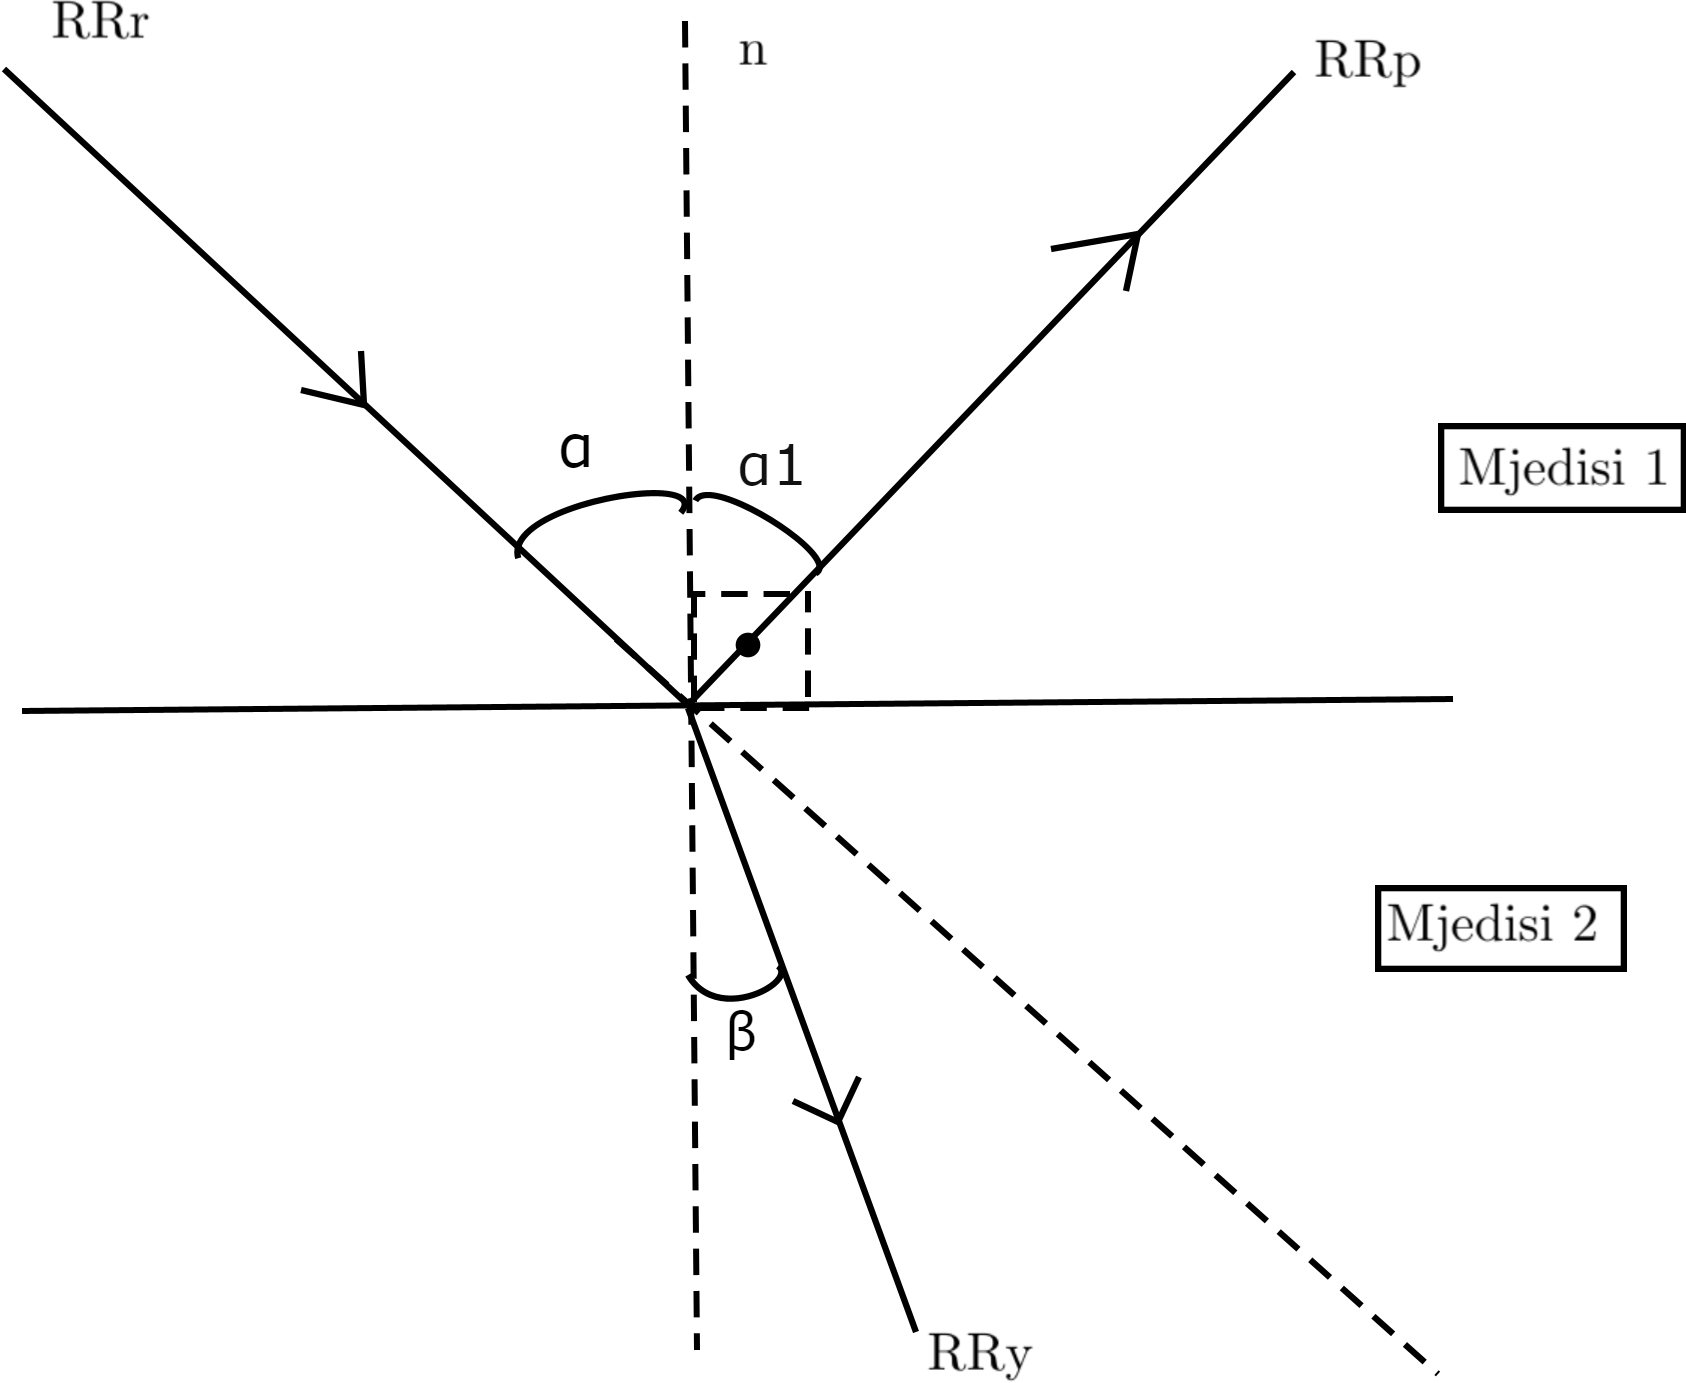
\includegraphics[width=80mm]{Imazhet/Pasqyrimi.png}
	\caption{Skicimi i një rrezeje dhe kalimi nga mjedisi 1 në mjedisin 2.}
	\label{fig:boat1}
\end{figure}

\begin{center}
	\textit{Simbolet:}\\
\end{center}

$RR_r \Rightarrow$ Rrezja rënëse.

$RR_p \Rightarrow $ Rrezja e pasqyruar.

$RR_y \Rightarrow $ Rrezja e përthyer.

$\alpha \Rightarrow$ Këndi i $RR_r$ .

$\alpha_1 \Rightarrow$ Këndi i $RR_p$ .

$\beta  \Rightarrow$ Këndi i $RR_y$ .

$n \Rightarrow$ Pingulja.\\

\begin{center}
	$\bullet$  \textbf{Përkufizim:}
\end{center}

Nëse mjedisi 2 është shumë i dendur atëherë këndi $\beta$ zvogelohet dhe i afrohet pingules ($\perp$) $n$.

Nëse mjedisi 2 është shumë pak i dendur atëherë këndi $\beta$ zmadhohet dhe i largohet  pingules ($\perp$) $n$.\\


$\bullet$\textbf{Pasqyrimi.}

$\alpha=\alpha_1$\\

$\bullet$ \textbf{Përthyerja.}

$\frac{sin \alpha}{sin \alpha_1}=\frac{v_1}{v_2}=\frac{n_1}{n_2}$


\begin{center}
	\textbf{Eksperimente:}
\end{center}

	\begin{figure}[h]
	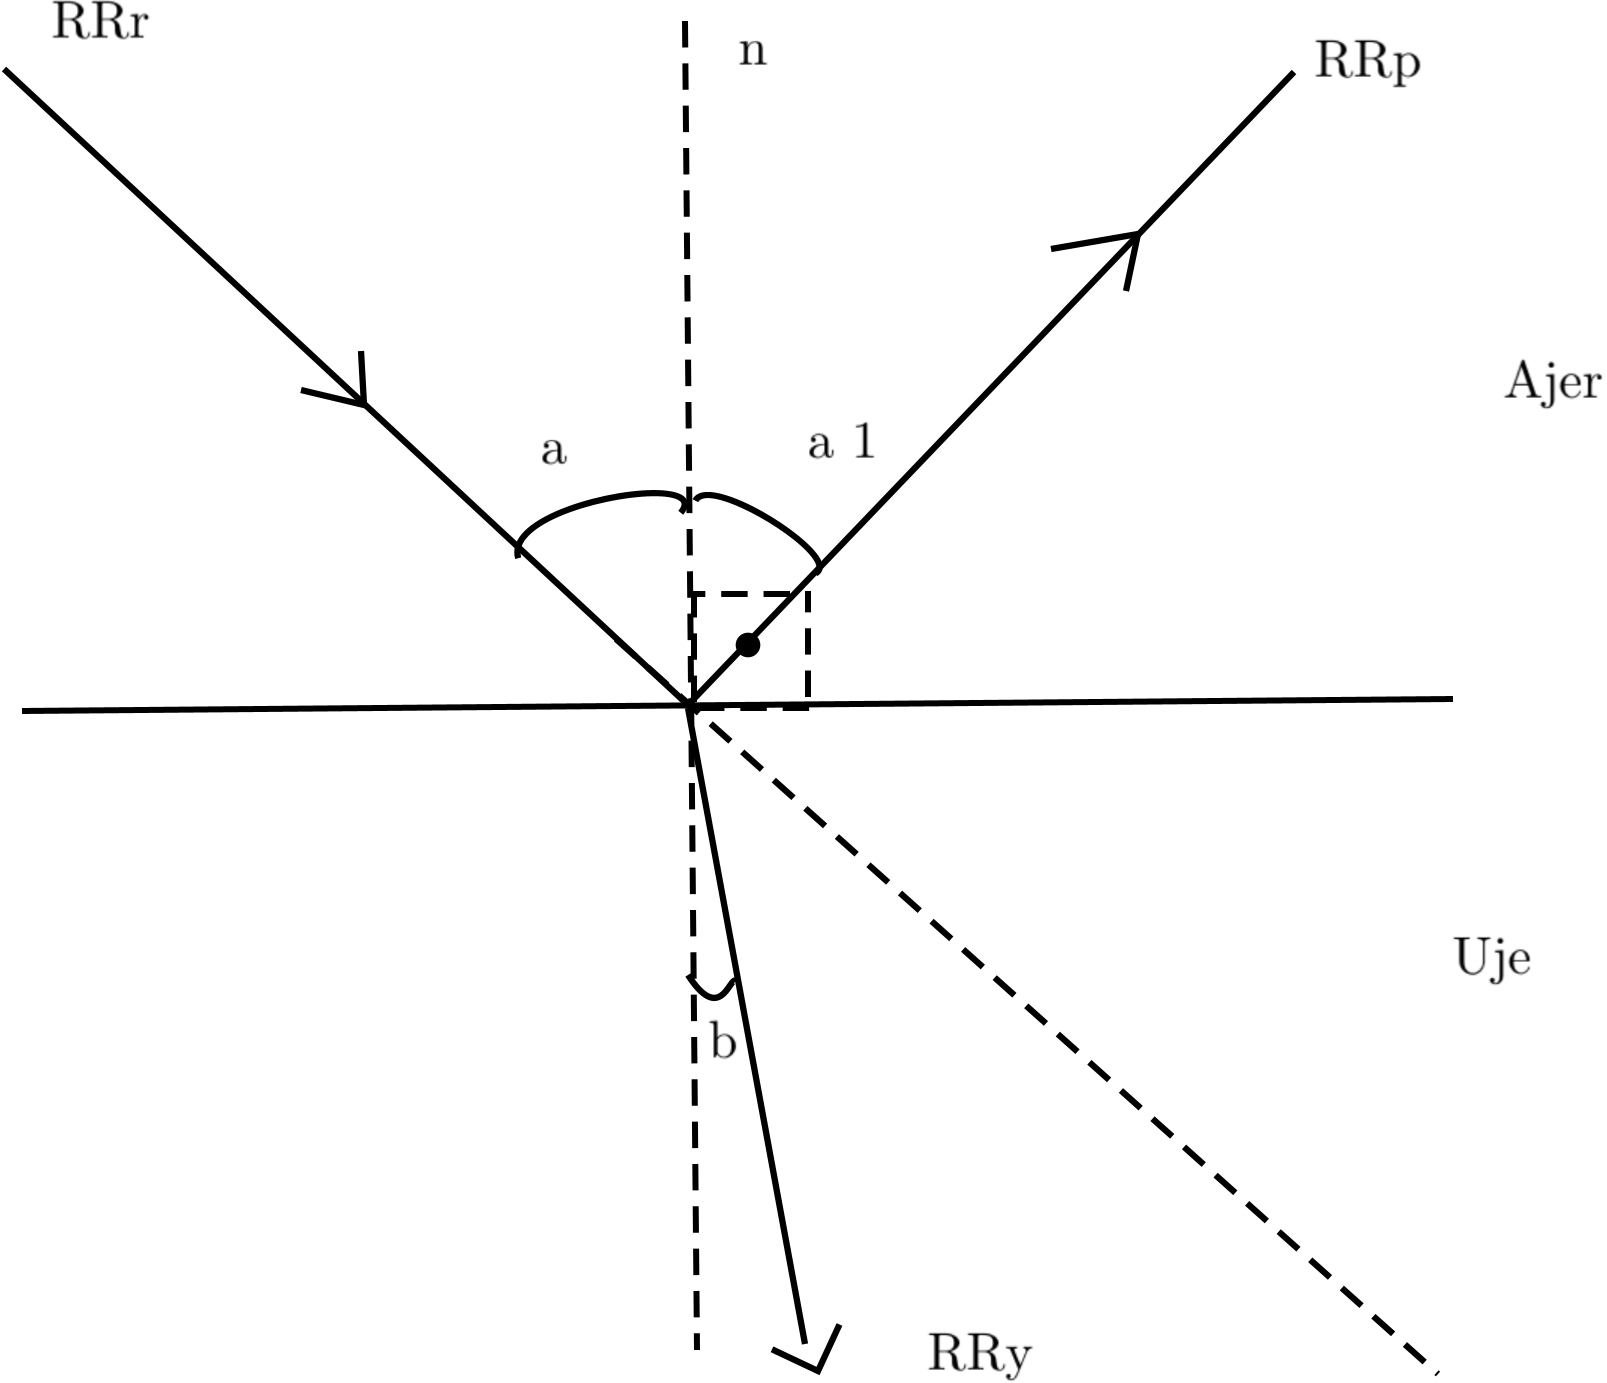
\includegraphics[width=80mm]{Imazhet/ajer uje.png}
	\caption{Skicimi i një rrezeje dhe kalimi nga mjedisi 1 në mjedisin 2.}
	\label{fig:boat1}
\end{figure}

Në figurën 44 tregohet kalimi i një rrezeje drite nga një mjedis jo i dëndur në një mjedis te dëndur.

	\begin{figure}[h]
	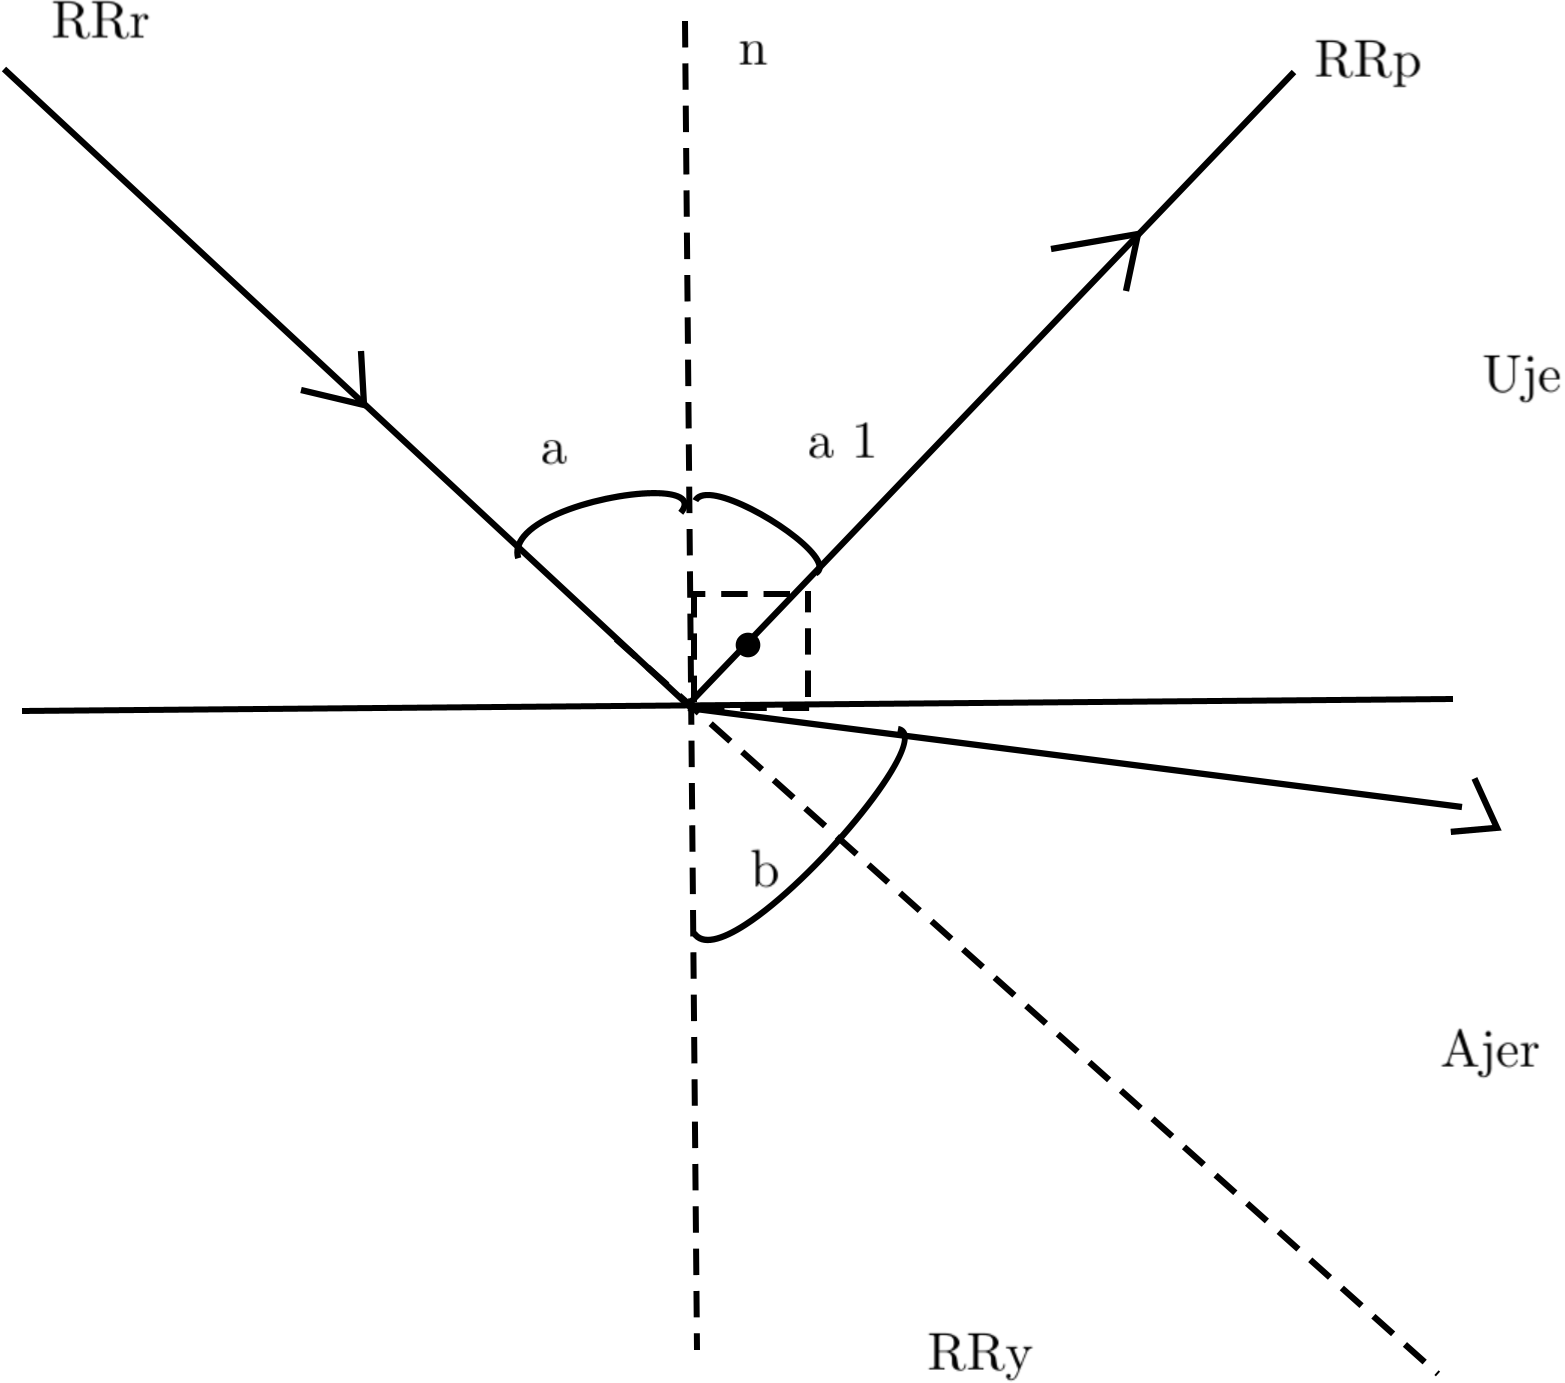
\includegraphics[width=80mm]{Imazhet/uje ajer.png}
	\caption{Skicimi i një rrezeje dhe kalimi nga mjedisi 1 në mjedisin 2.}
	\label{fig:boat1}
\end{figure}

Në figurën 45 tregohet kalimi i një rrezeje drite nga një mjedis i dendur në një mjedis jo të dendur.

$\bullet$ \textbf{Reflektimi.}

$n=\frac{c}{v}$

$c \Rightarrow$ Shpejtësia në vakum.

$v \Rightarrow$ Shpejtësia në mjedis.

$\bullet$ \textbf{Pasqyrimi i plotë.}

$\frac{sin\alpha_k}{sin90^\circ}$=$\frac{n_2}{n_1}$ ,(sin$90^\circ=1$)


\begin{center}
	\textbf{Eksperimente.}
\end{center}
Ne figuar e meposhteme do te ilustrojm disa  nga pasqyrimet e rrezes se dritese ne trupa te ndryshem gjeometrik.Ndertimi i pasqyrimit te rrezes se drites eshte shume i thjesht por duhet te kemi kujdes kur kemi nje trup te dendur dhe nje trup jo te dendur kendi $\beta$ duhet te ndertohet me kujdes qe pasqyrimi te jete sa me i sakte.Kalimi nga ajri ne nje mjedis tjeter me te dendur e zvogelon kendin $\beta$ ndersa kalimi nga nje mjedis i dendur s.p.sh uji ne nje mjdesi me pak te dendur s.p.sh ajri kendi $\beta$ do te kete vlera me te medha.
\begin{center}
$\bullet$ \textbf{Ajer $\Rightarrow$ Qelq $\Rightarrow$ Ajer.}
	

\end{center}

\begin{center}
	Kuboidi:
\end{center}
\begin{figure}[h]
	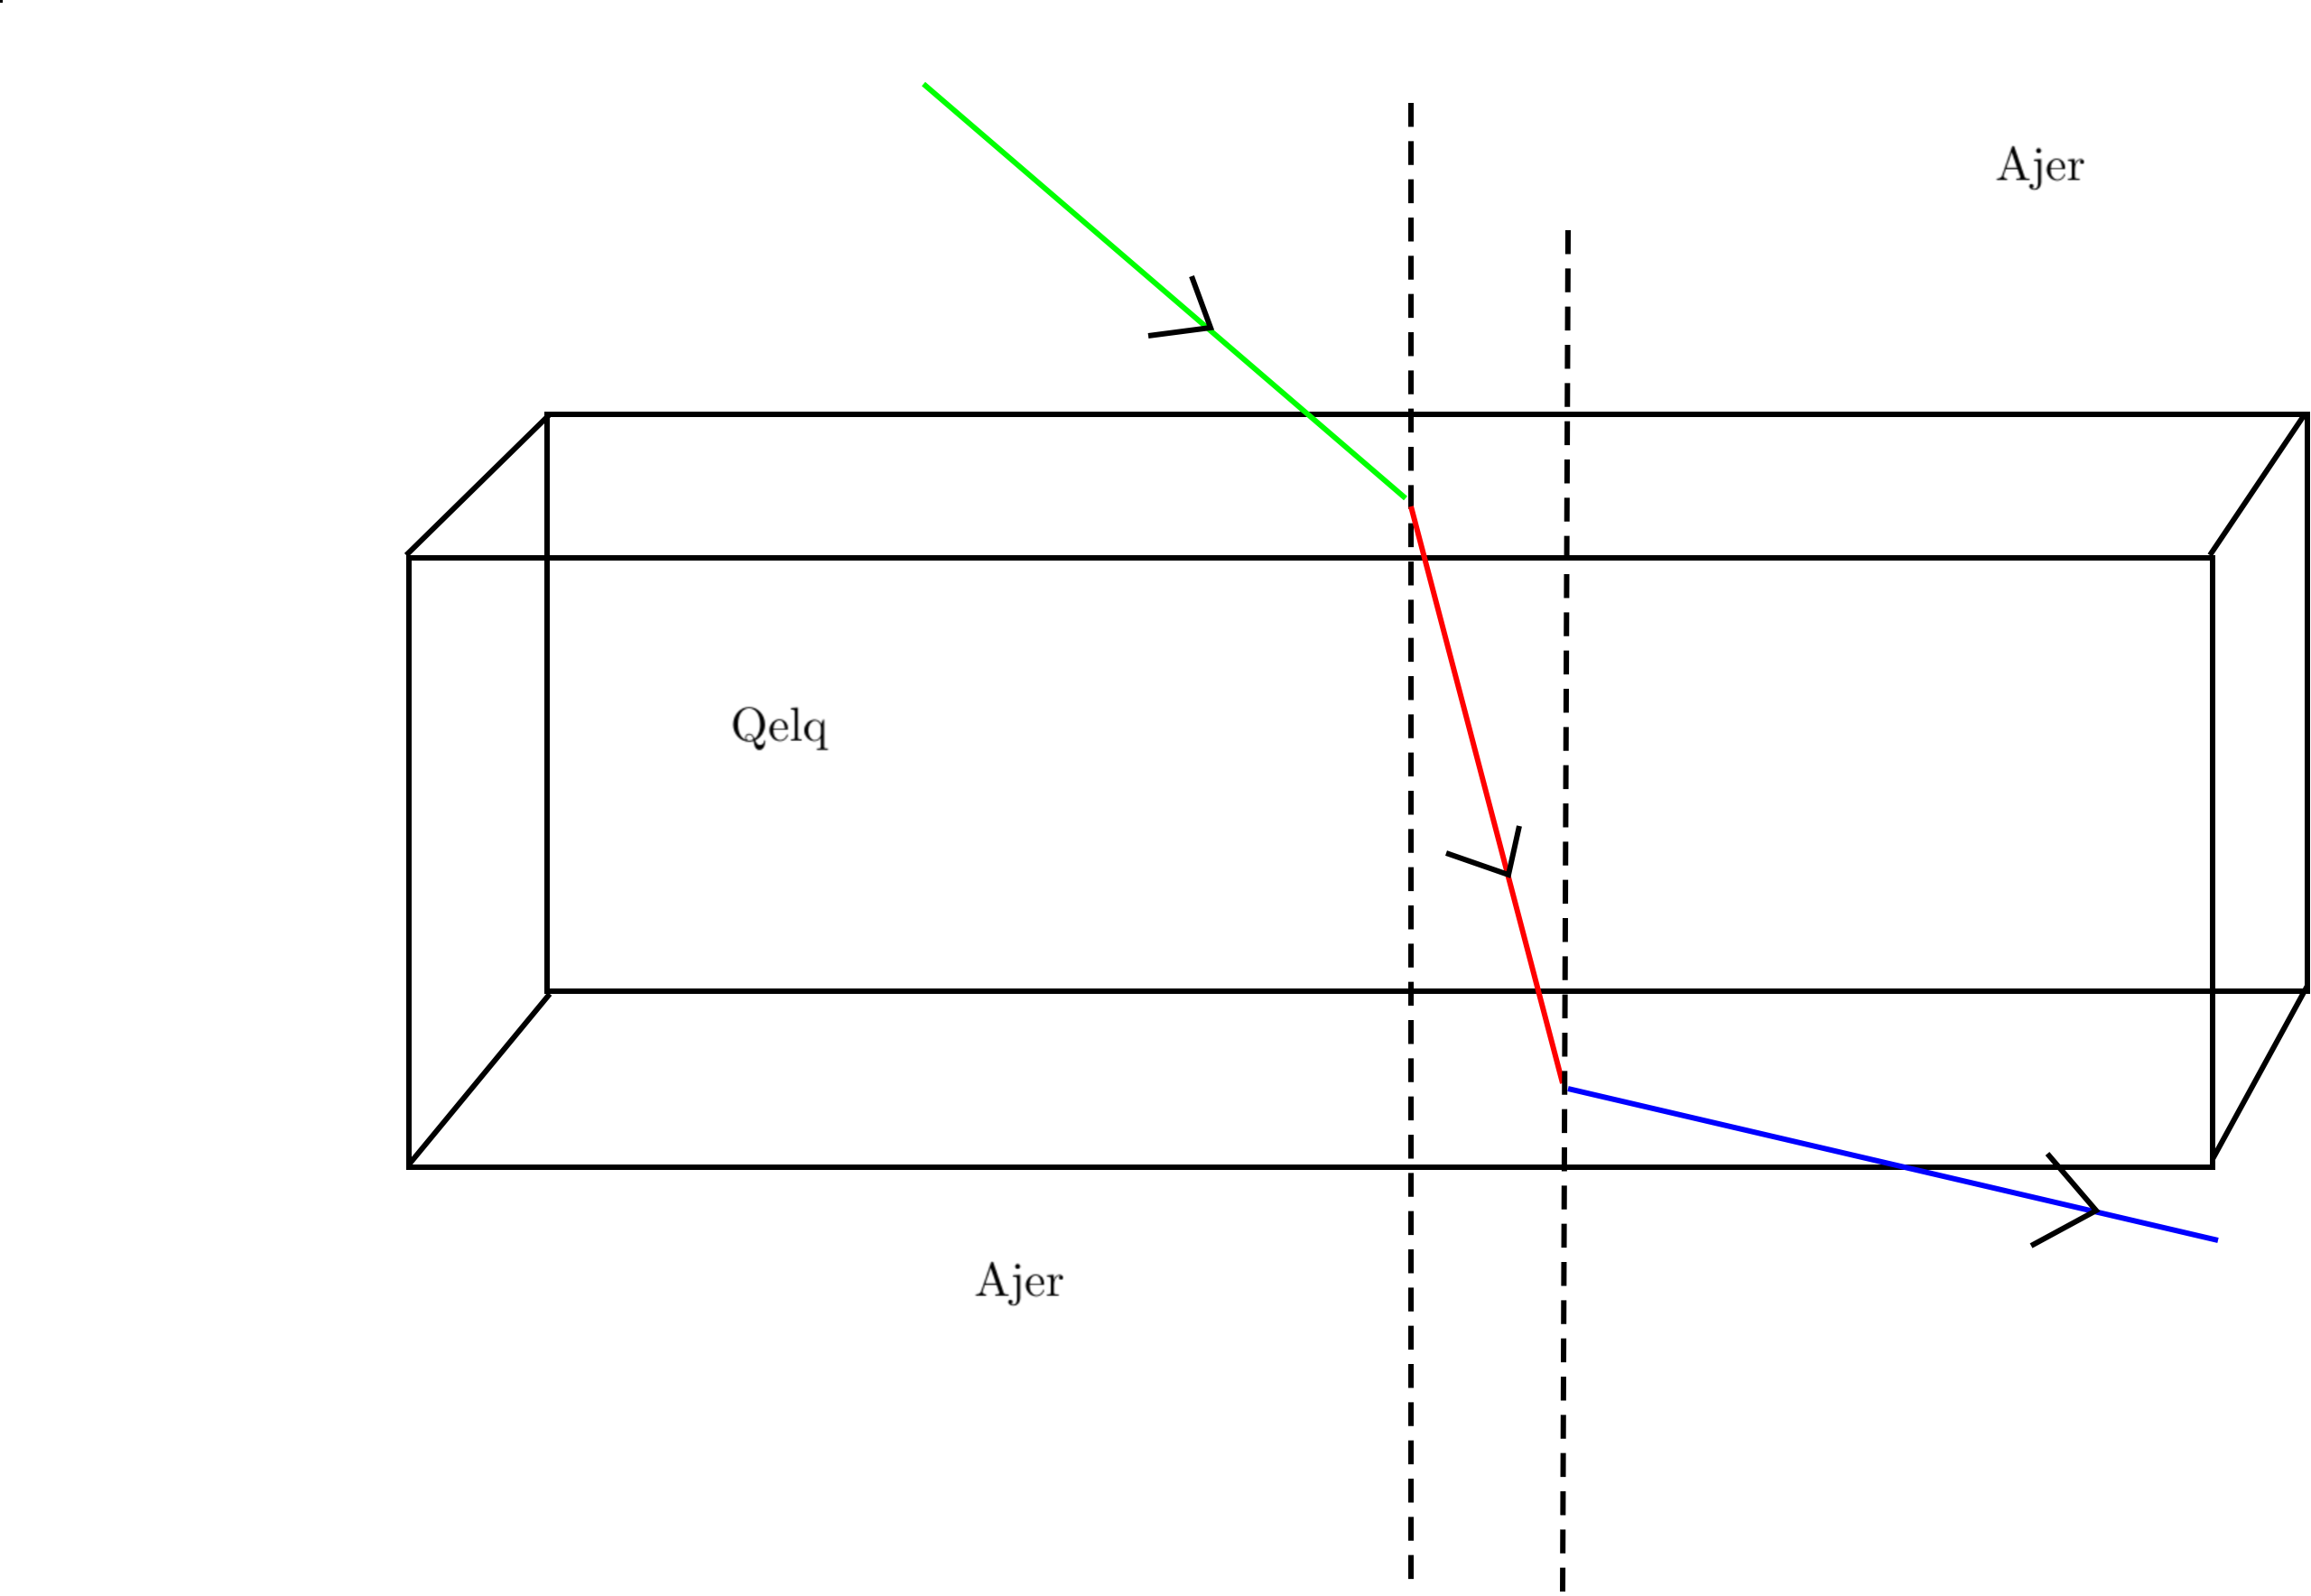
\includegraphics[width=70mm]{Imazhet/ajer-qelq-ajer.png}
	\caption{Kalimi i nje rrezeje drite nga ajri ne qelq dhe perseri ne ajer.}
	\label{fig:boat1}
\end{figure}

\begin{center}
	Prizmi:
\end{center}
\begin{figure}[h]
	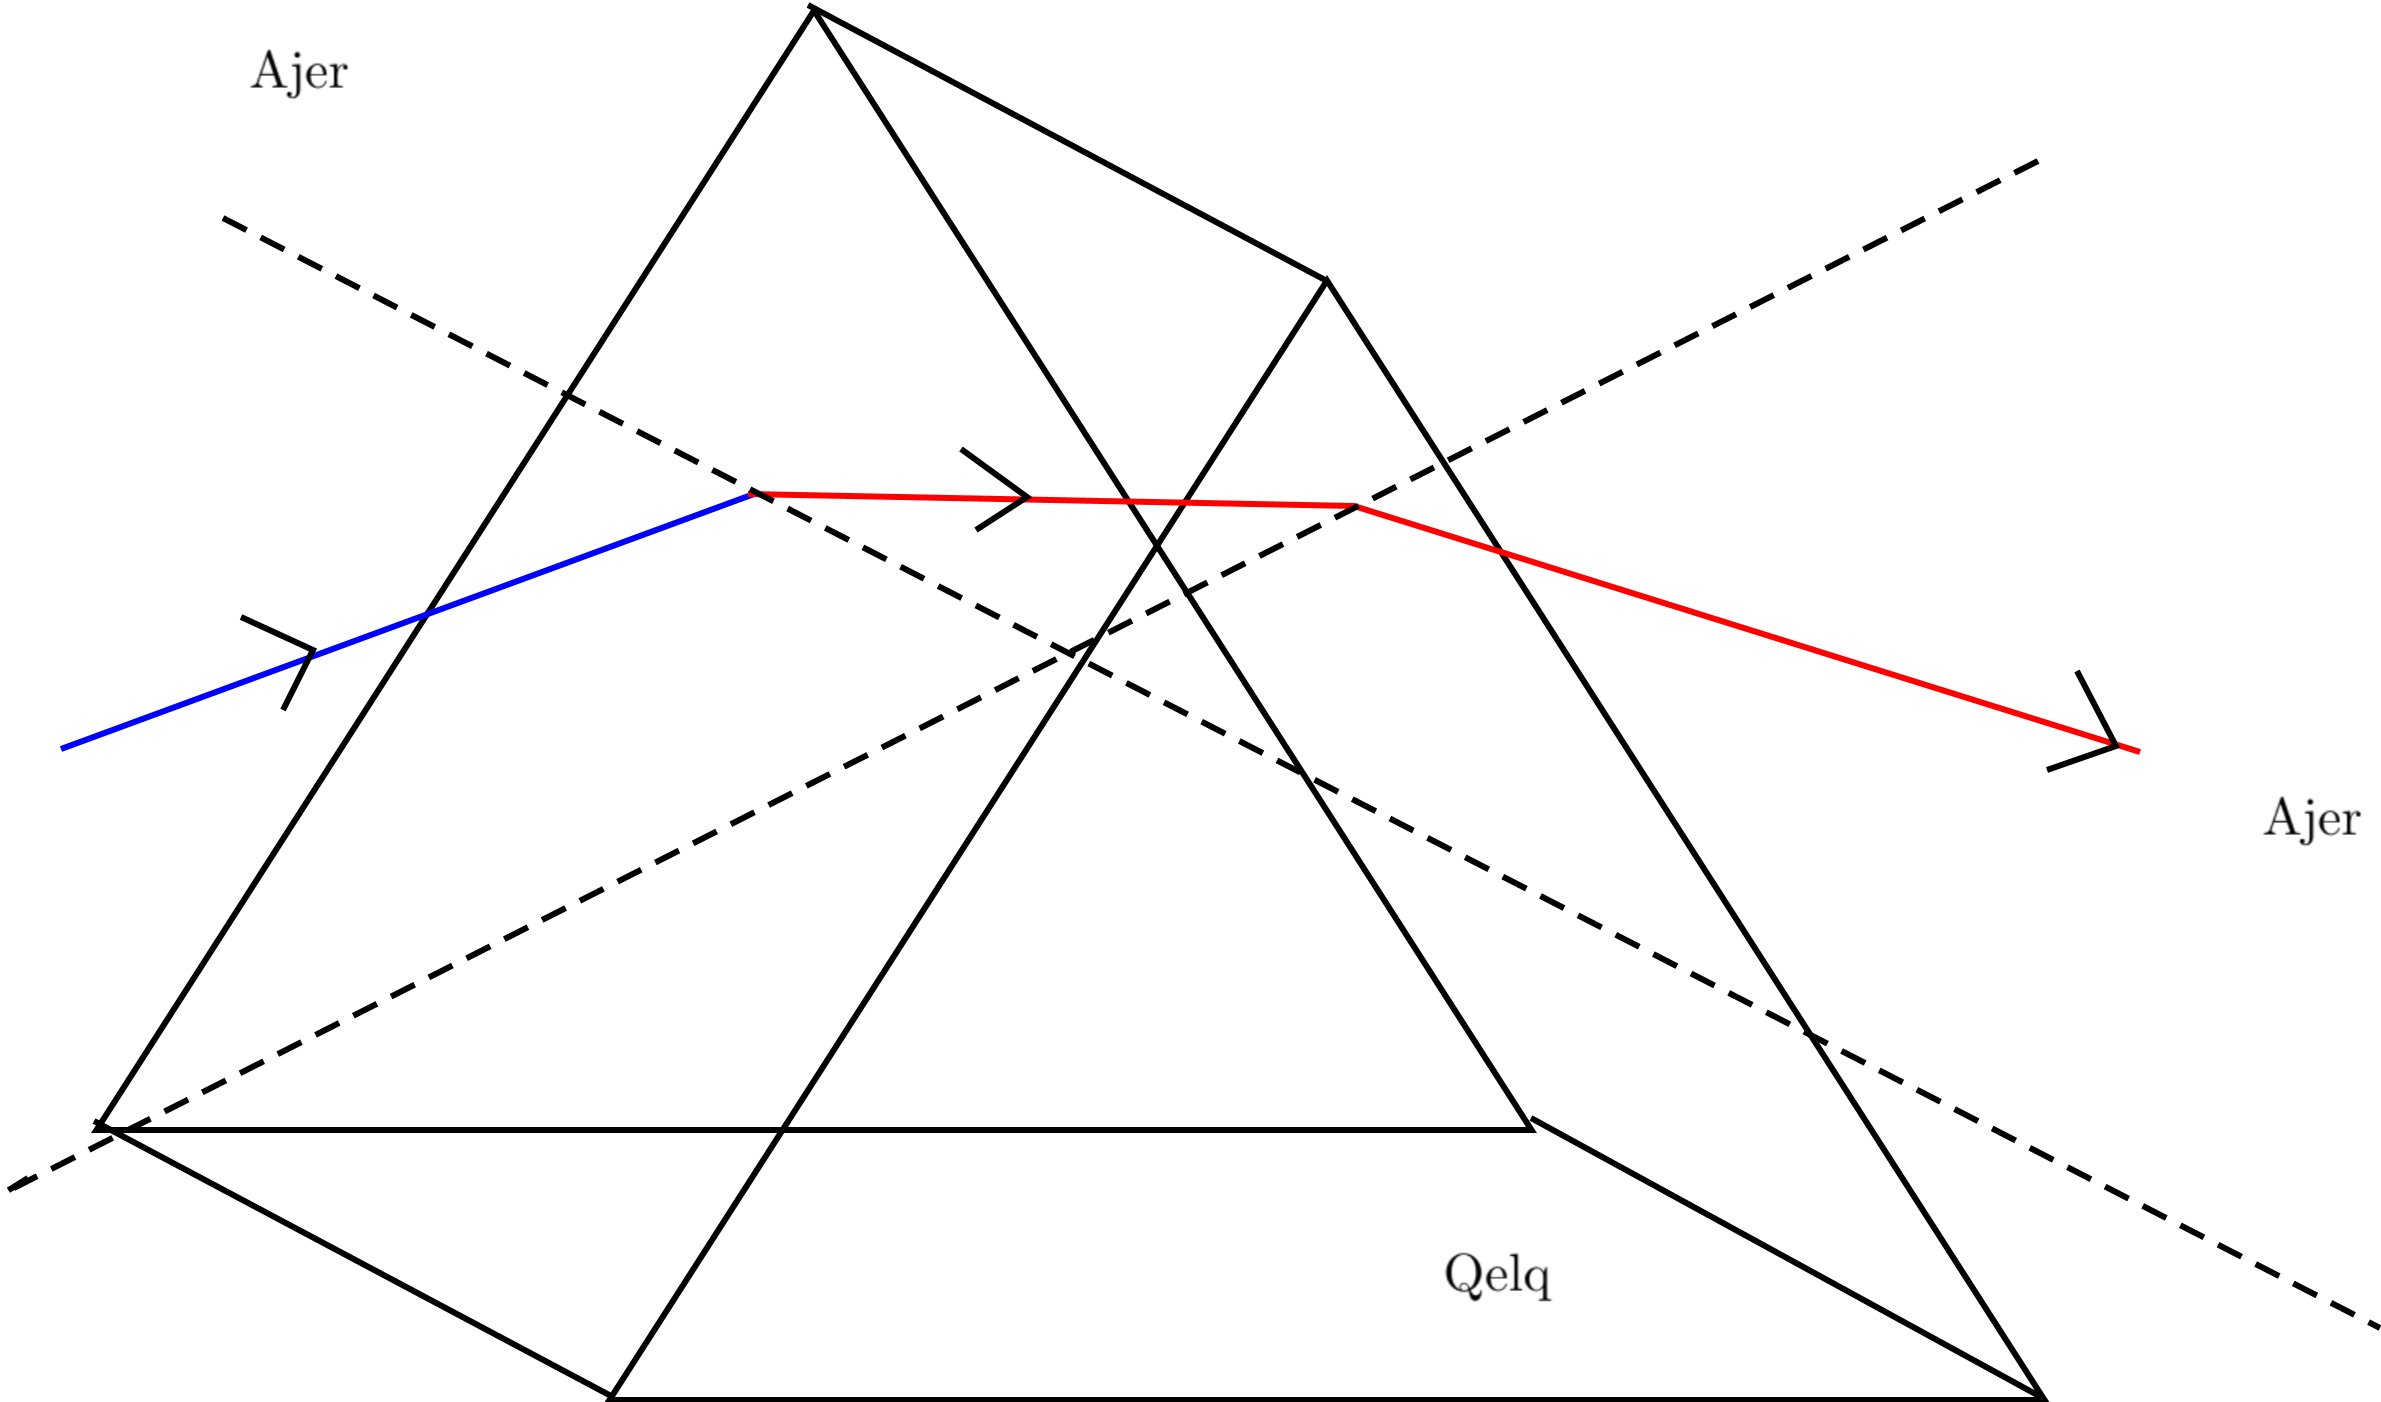
\includegraphics[width=70mm]{Imazhet/ajer-qelqprizmi-ajer.png}
	\caption{Kalimi i nje rrezeje drite nga ajri ne qelq dhe perseri ne ajer.}
	\label{fig:boat1}
\end{figure}

\section{Shembellimet.}

\begin{center}
$\bullet$	\textbf{Pasqyra e rrafshet.}
\end{center}
$\bullet$ \textbf{Karakteristikat e shembellimit ne pasqyren e rrafshet.}

1.Shembellimi dhe objekti kane nje largesi te barabarte nga pasqyra.

2.Permasat e shembellimit dhe objektit jane te barabarta.

3.Shembellimi eshte gjithmone virtual.

\textbf{Cfare quajm shembellim virtual dhe shembellim real?}

Shembellimm real quajm dukurin kur rrezet ndodhen ne piken e prerjes se tyre kur ato jan te pasqyruara ose te perthyera.

Shembellim virtual quajm dukurin kur ndodhet ne zgjatimin e rrezeve te pasqyruara ose te perthyera.

\begin{figure}[h]
	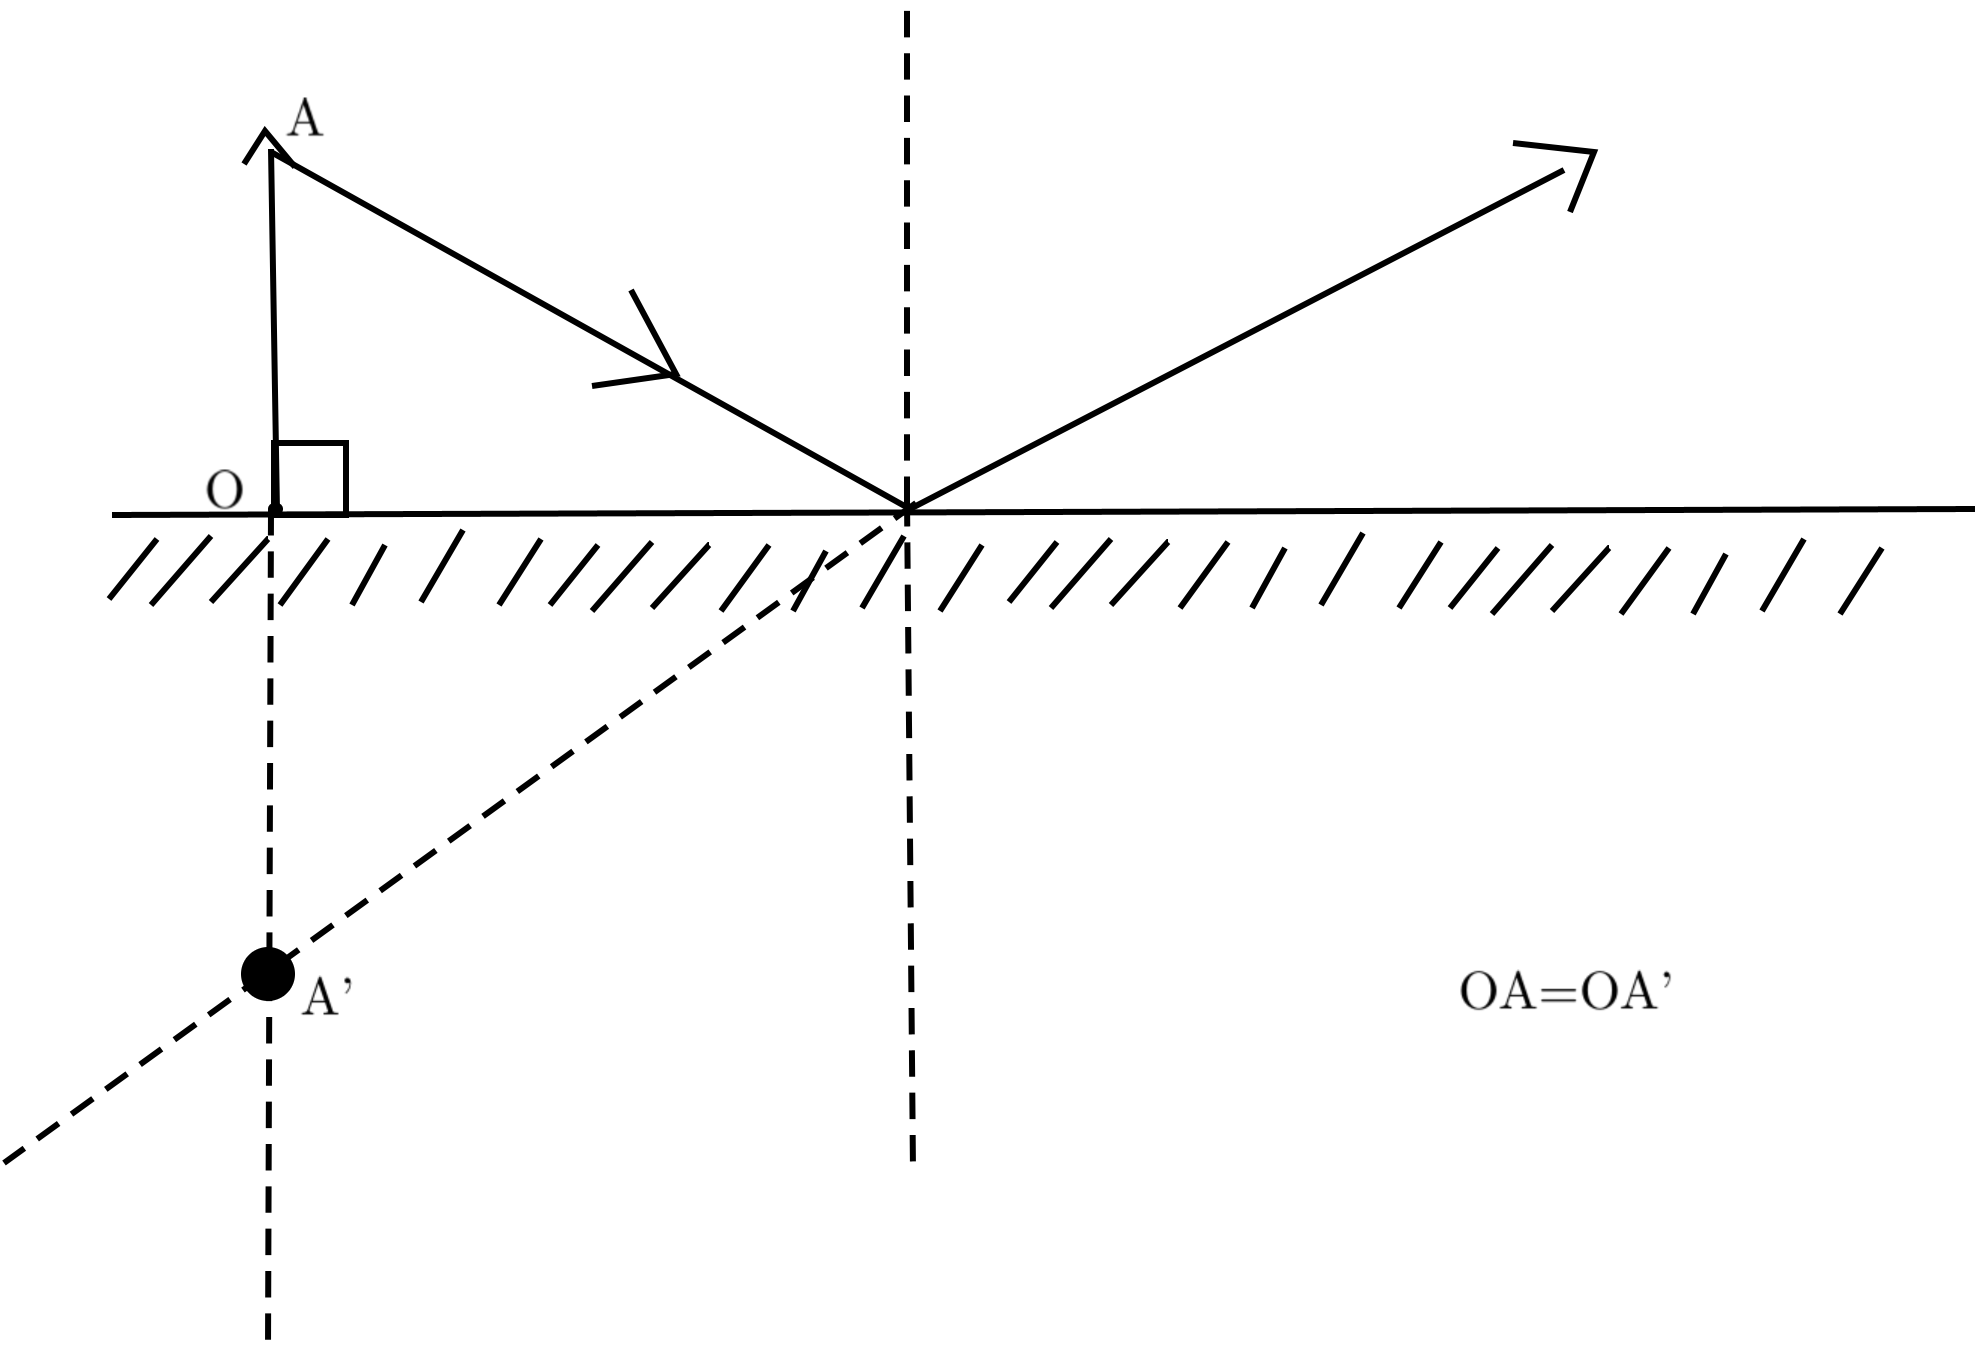
\includegraphics[width=70mm]{Imazhet/pasqyra e rrafshet.png}
	\caption{Pasqyra e rrafshet dhe pasqyrimi i objektit.}
	\label{fig:boat1}
\end{figure}

\begin{center}
$\bullet$	\textbf{Pasqyra sferike.}
\end{center}


\begin{figure}[h]
	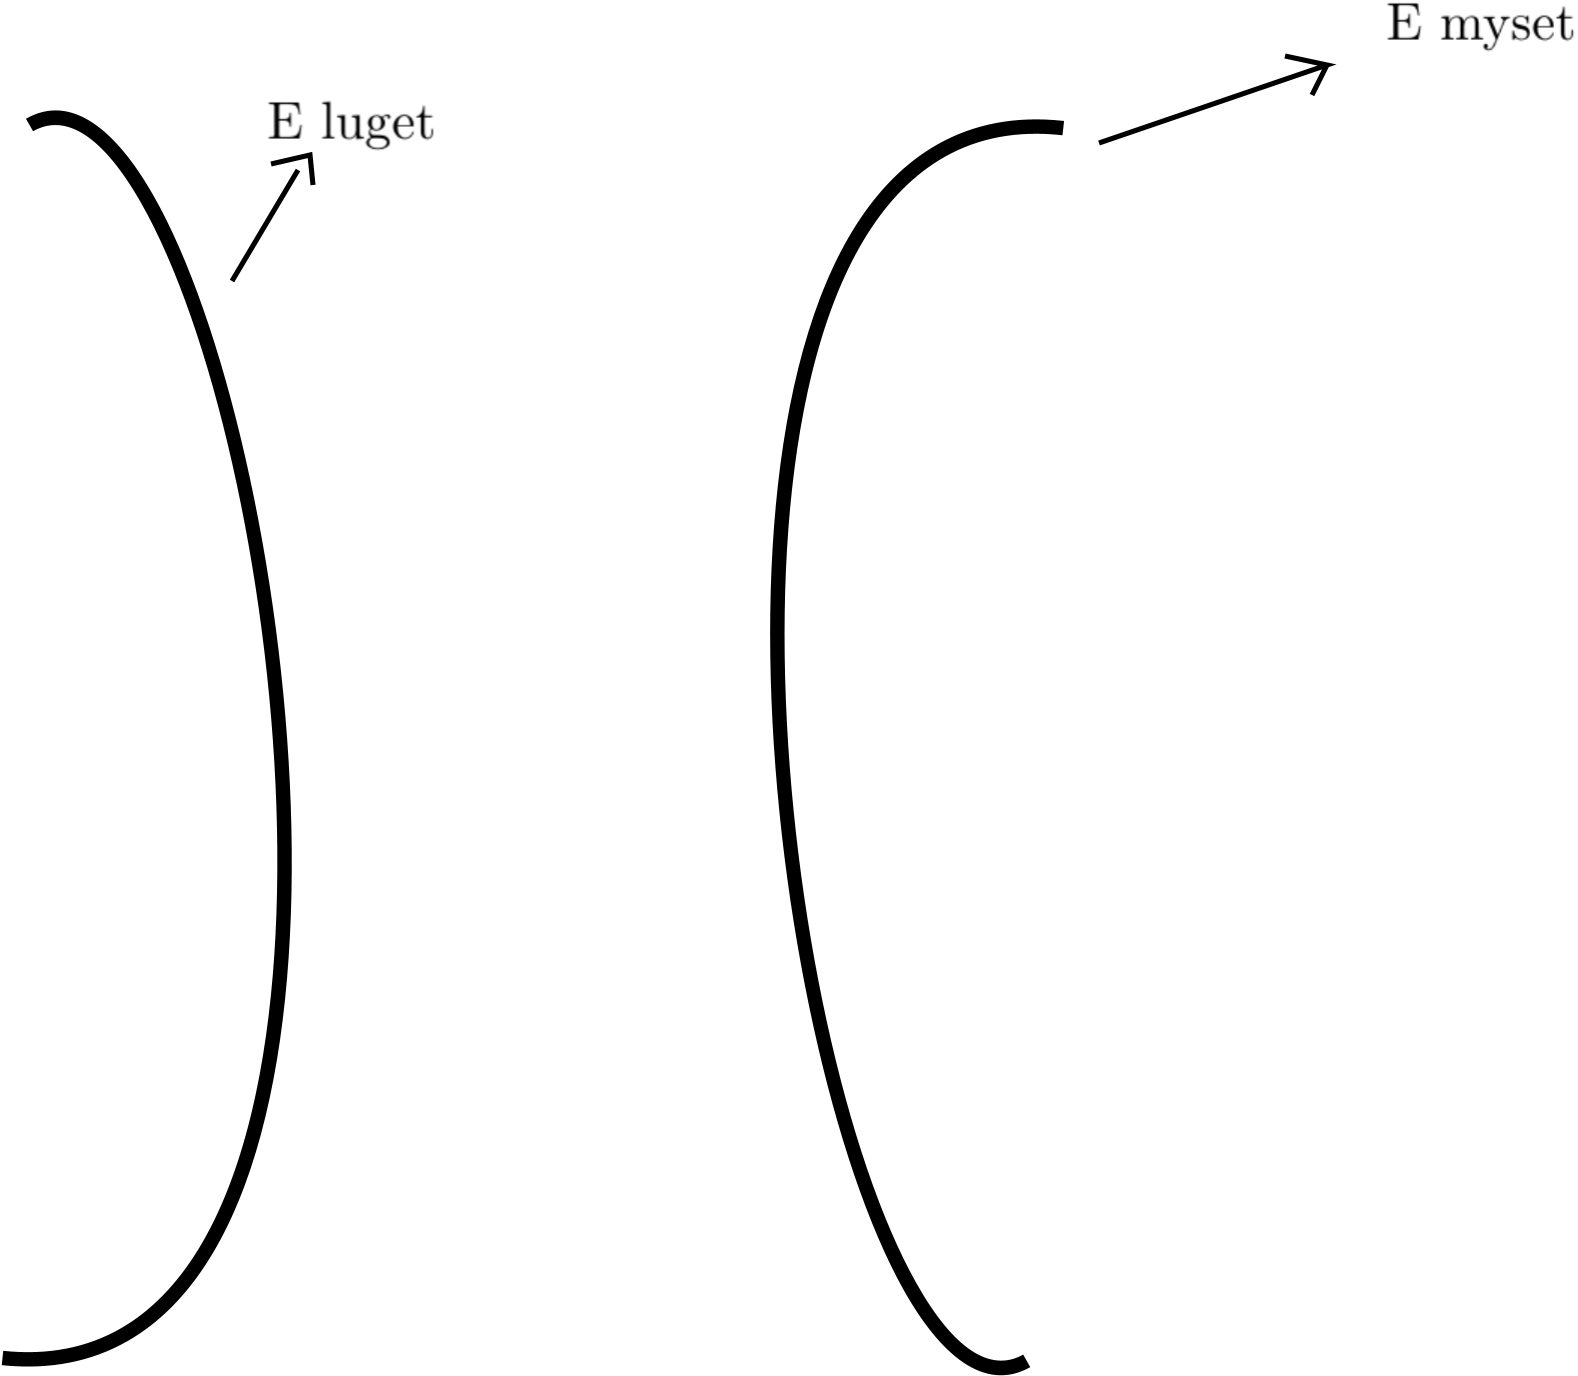
\includegraphics[width=62mm]{Imazhet/pasqyra sferike e luget dhe myset.png}
	\caption{Pasqyra sferike e luget dhe e mystet.}
	\label{fig:boat1}
	\end{figure}


\begin{center}
	\underline{Pasqyra sferike e luget dhe ndertimi i saj.}
\end{center}
\begin{figure}[h]
	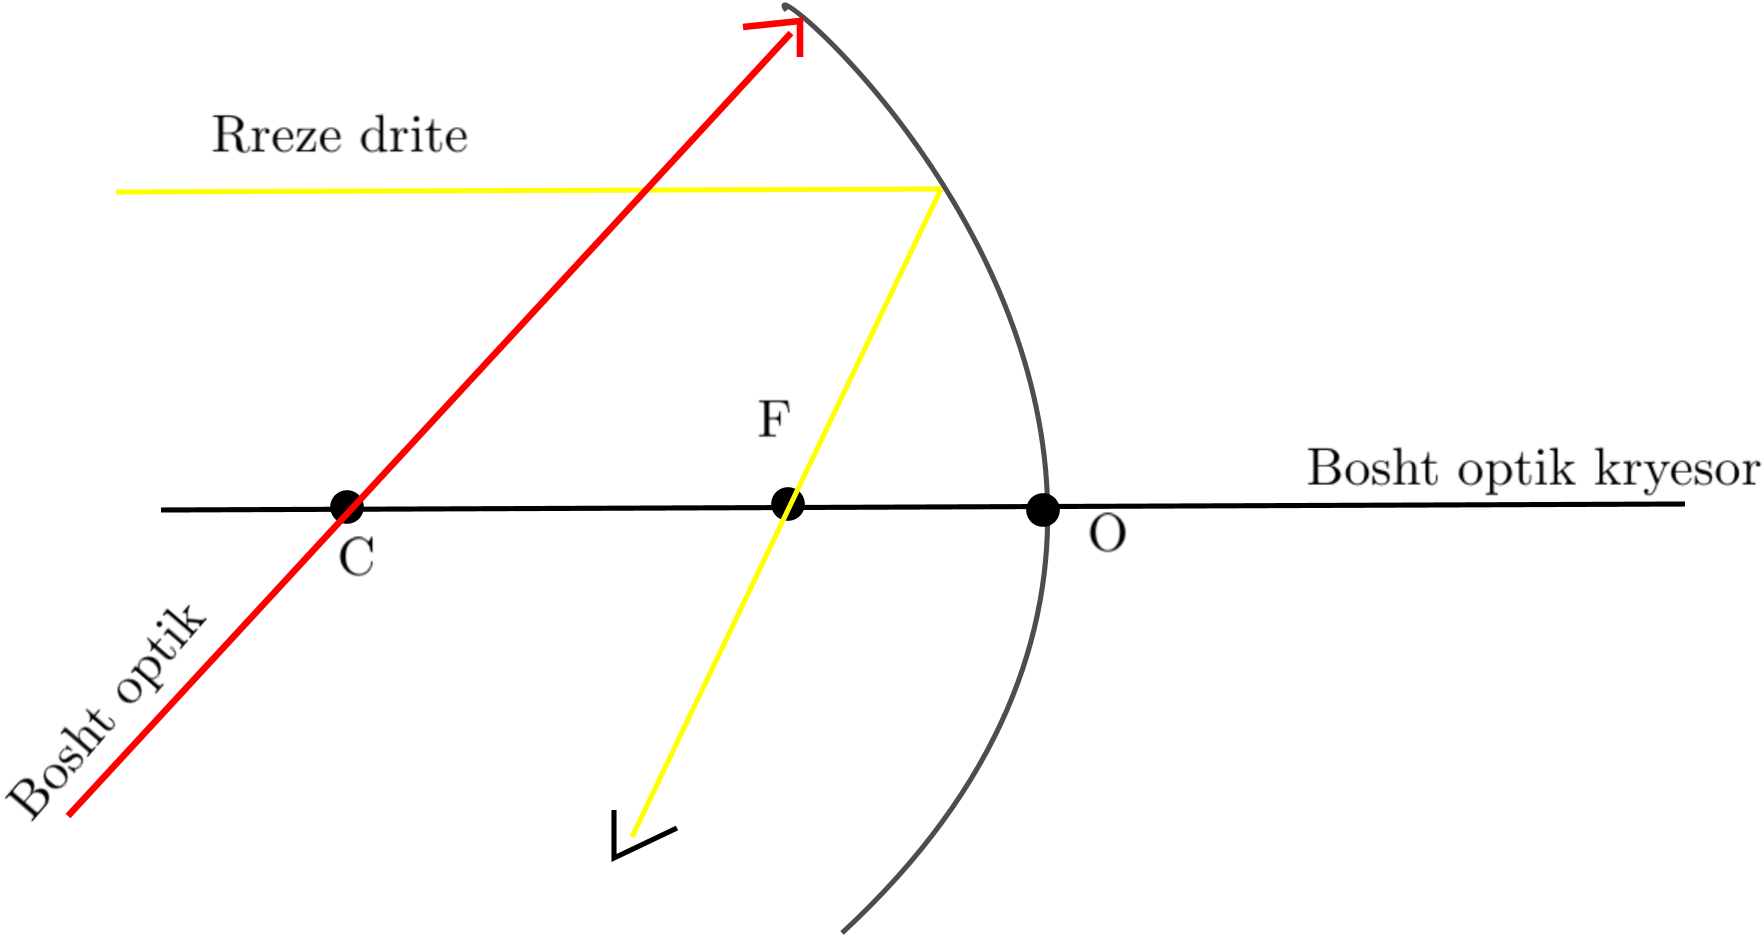
\includegraphics[width=80mm]{Imazhet/pasqyra sferike e luget.png}
	\caption{Pasqyra sferike e luget.}
	\label{fig:boat1}
\end{figure}

\begin{center}
	\textit{Simbolet:}
\end{center}

$F \Rightarrow $ Vatra.

$r \Rightarrow$ Rrezja.



\begin{center}
	Formula:
\end{center}

$F=\frac{r}{2}$

 \begin{center}
 	\underline{Pasqyra sferike e myset dhe ndertimi i saj.}
 \end{center}
 \begin{figure}[h]
 	\includegraphics[width=80mm]{Imazhet/pasqyra sferike e myset.png}
 	\caption{Pasqyra sferike e myset.}
 	\label{fig:boat1}
 \end{figure}

Pasqyra e myset ka vetin ti shperndaje rrezet keshtuqe vetem zgjatimet e tyer takohen ne vatren($F$).\\


\begin{center}
	\textbf{\underline{Shembellimi i pasqyres sferike.}}
\end{center}

Per ndertimin e shembellimit sherbejn keto rregulla.

1.Rrezja paralele me boshtin optike kryesor e cila pas pasqyrimit kalone ne vatren ($F$).

2.Rrezja qe kalon ne vater pas pasqyrimit kthehet paralele me boshtin e tij kryesor.

3.Rrezja qe kalone neper qendren e pasqyres kthehet ne te njejtin drejtim sepse bie pingule $\perp$.

4.Rrezet paralele $\parallel$ me boshtin optike pas pasqyrimit do te kalojne aty ku boshti optik pret rrafshin katror.

\begin{center}
	$\bullet$ Raste te ndryshme.\\
\end{center}


1.Objekti ndodhet ne nje largesi me te madhe se vatra.

 \begin{figure}[h]
	\includegraphics[width=80mm]{Imazhet/Objekti_ndodhet_ne_nje_largesi_me_te_madhe_se_vatra.png}
	\caption{Objekti ndodhet ne nje largesi me te madhe se vatra.}
	\label{fig:boat1}
\end{figure}

Shembellimi eshte:

Real.

I zvogeluar.

I permbysur.\\



2.Objekti ndodhet ndermjet vatres dhe pasqyres.\\


Shembellimi eshte:

Virtual.

I zmadhuar.

I drejt.\\

 \begin{figure}[h]
	\includegraphics[width=80mm]{Imazhet/Objekti_ndodhet_ndermjet _vatres_dhe_pasqyres.png}
	\caption{Objekti ndodhet ndermjet vatres dhe pasqyres.}
	\label{fig:boat1}
\end{figure}

3.Shembellimi i nje objekti para nje pasqyre te myset.\\


Shembellimi eshte:

Virtual.

I zvogeluar.

I drejt.\\

\begin{figure}[h]
	\includegraphics[width=80mm]{Imazhet/Shembellimi_i_nje_objekti_para_nje_pasqyre_te_myset.png}
	\caption{Shembellimi i nje objekti para nje pasqyre te myset.}
	\label{fig:boat1}
\end{figure}


\section{Thjerrat.}
Kemi 2 lloje thjerrash.\\

\textbf{1.Thjerra permbledhese.}

\begin{figure}[h]
	\includegraphics[width=60mm]{Imazhet/thierra_permbledhese.png}
	\caption{Skicimi i thierres permbledhese.}
	\label{fig:boat1}
\end{figure}

Thjerra permbledhese sic kuptohet dhe nga emri mbledh te gjitha rrezet ne vater(F) pra ne nje pike.\\

\begin{figure}[h]
	\includegraphics[width=60mm]{Imazhet/thierra_permbledhese_F.png}
	\caption{Skicimi i thierres permbledhese.}
	\label{fig:boat1}
\end{figure}



\textbf{2.Thjerra shperndarse.}



\begin{figure}[h]
	\includegraphics[width=55mm]{Imazhet/thjerra_shperndarse_F.png}
	\caption{Skicimi i thierres shperndarse.}
	\label{fig:boat1}
\end{figure}


Thjerra shperndarse sic kuptohet dhe nga emri shperndan te gjitha rrezet dhe vetem zgjatimet e tyre takohen ne vater(F) pra ne nje pike.

\begin{figure}[h]
	\includegraphics[width=80mm]{Imazhet/thjerra_shperndarse.png}
	\caption{Skicimi i thierres shperndarse.}
	\label{fig:boat1}
\end{figure}


\begin{center}
	$\bullet$ Raste te ndryshme.\\
\end{center}



\textbf{1.Objekti ndodhet brenda  2 fishit te vatres.}\\

\begin{figure}[h]
	\includegraphics[width=90mm]{Imazhet/thj1.jpg}
	\caption{Skicimi i thierres shperndarse.}
	\label{fig:boat1}
\end{figure}

Ne kete rast objekti ndodhet brenda 2 fishit te vatres(F).Dhe shembellimit nga vatra del real,i permbysur,i zmadhuar.\\


\textbf{2.Ndodhet pertej 2 fishit te vatres.}\\
Ne kete rast objekti ndodhet jashte 2 fishit te vatres(F).Dhe shembellimit nga vatra del real,i permbysur,i zvogeluar.

\begin{figure}[h]
	\includegraphics[width=90mm]{Imazhet/thj2.jpg}
	\caption{Skicimi i thierres shperndarse.}
	\label{fig:boat1}
\end{figure}


\textbf{3.Objekti ndodhet brenda vatres(F).}

Ne kete rast objekti ndodhet brenda  vatres(F).Dhe shembellimit nga vatra del virtual,i drejt,i zmadhuar.
\begin{figure}[h]
	\includegraphics[width=70mm]{Imazhet/thj3.jpg}
	\caption{Skicimi i thierres shperndarse.}
	\label{fig:boat1}
\end{figure}

\begin{center}
\textit{	Simbolet:}
\end{center}

$d \Rightarrow $ Largesia e objektit.

$d' \Rightarrow$ Largesia e shembellimit.

$f \Rightarrow$ Largesia vatrore.

$k \Rightarrow $ Zmadhimi i koeficentit.

$y \Rightarrow$ Gjatesia e objektit.

$y' \Rightarrow$ Gjatesia e shembellimit.

$D \Rightarrow$ Fuqia optike.(Dioptri)

$n \Rightarrow$ treguesi i perthyerjes se thjerres.

$R \Rightarrow$ Rrezja e siperfaqes.

\begin{center}
	1-Thjerra permbledhese:(Formulat)
\end{center}

$\frac{1}{d}+\frac{1}{d'}=\frac{1}{f}$  (Shembellimi real)

$\frac{1}{d}-\frac{1}{d'}=\frac{1}{f}$  (Shembellimi virtual)


\begin{center}
	2-Thjerra shperndarse:(Formulat)
\end{center}

$\frac{1}{d}-\frac{1}{d'}=-\frac{1}{f}$ 

\begin{center}
	ose
\end{center}

$\frac{1}{d'}-\frac{1}{d}=\frac{1}{f}$ 

\begin{center}
	Formula te tjera:
\end{center}

$k=\frac{y'}{y}=\frac{d'}{d}=\frac{d'-f}{f}$

$D=\frac{1}{f}$


\section{Fizika kuantike.}

\begin{center}
	\textit{Simbolet:}
\end{center}

$E \Rightarrow$ Kunat energjie.

$h \Rightarrow$ Konstante $\approx$ $6,62 \cdot 10^{-34} J/s$

$\sigma \Rightarrow$ Stefan-Boltzmann konstante $\approx$$5,67 \cdot 10^{-8} W/m^2 \cdot K^4$

$T \Rightarrow$ temperatura termodinamike.

$f \Rightarrow$ Frekuenca ($H_z$).

\begin{center}
	Formulat:
\end{center}

$E=h \cdot f$

$h \cdot f= E_k +A_d $ Ekuacioni i Anjshtajnit.(Largohen fotonet)

$h \cdot f=A_d $ Ekuacioni i Anjshtajnit.(Nuk largohen fotonet)

$E= \sigma \cdot T^4$

\begin{center}
	Fotoefekti:
\end{center}

Qe te ndodh fotoefekti $A_d>A$ ose $A_d=A$.

\begin{center}
	\textit{Simbolet:}
\end{center}

$c \Rightarrow$ Shpejtesia e drites $\approx$ $3 \cdot 10^8 m/s$.

$U_0 \Rightarrow$ Tension frenimi.

$P \Rightarrow$ Impulsi(De brojnit).

\begin{center}
	Formulat:
\end{center}

$c= \lambda \cdot f$

$f= \frac{c}{\lambda}$

$\frac{h \cdot c }{\lambda}=A_d$

$U_0 = \frac{h \cdot c}{\lambda \cdot e}$

$P=\frac{h}{\lambda}$

$\lambda = \frac{h}{\sqrt{2 \cdot e \cdot U_0 \cdot m_e}}$

\section{Fizika berthamore.}

\begin{figure}[h]
	\includegraphics[width=70mm]{Imazhet/berthama.png}
	\caption{Berthama e atomit.}
	\label{fig:boat1}
\end{figure}

$X^A_Z$

\begin{center}
	\textit{Simbolet:}
\end{center}

$A \Rightarrow $ Numri i mases.(Z+N)

$Z \Rightarrow$ Numri i ngarkeses.

$E_L \Rightarrow$ Energjia e lidhjes.

$E_B \Rightarrow$ Energjia e berthames.

$E_p \Rightarrow$ Energjia e protonit.

$E_n \Rightarrow$  Energjia e neutronit.


\begin{center}
	Formulat:
\end{center}

$E_L =E_B - E_p - (A-Z)E_n$

$E_L = m_B \cdot c^2 - Z m_p \cdot c^2 - (A-Z) \cdot m_n \cdot c^2$

$E_L= (m_b - Zm_p-(A-Z)m_n) c^2$

$\Delta m = \frac{E_L}{c^2} $

$E_L=\Delta m \cdot c^2$

$E=m \cdot c^2$

\begin{center}
	Ligjet e reaksioneve:
\end{center}

Kemi dy lloje reaksionesh te vetvetishme,te detyruara.\\

$\bullet$ \textbf{Grimcat qe leshohen nga reaksionet berthamore.}

1-Reaksioni $\alpha$ ($H^4_2e$)(+) $\Rightarrow$ $X^A_Z \Rightarrow y^{A-4}_{Z-2} + \alpha (H^4_2e)$.

2-Reaksioni -$\beta$ ($e^{-}$) (-) $\Rightarrow$ $X^A_Z \Rightarrow y^A_{Z+1} + e^0_{-1}$.

3-Reaksioni +$\beta$ ($e^{+}$) (+) $\Rightarrow$ $X^A_Z \Rightarrow y^A_{Z-1} + e^0_{+1}$.

4-Reaksioni $\gamma ^0_0$ (f) (0) $\Rightarrow$ nuk ka.\\

\begin{figure}[h]
	\includegraphics[width=70mm]{Imazhet/reaksionet_.png}
	\caption{Reaksinet.}
	\label{fig:boat1}
\end{figure}

$\bullet$ \textbf{Ligjet e ruajtjes.}

1-Ligji i ruajtjes se energjis.

2-Ligji i ruajtjes se impulsit.

3-Ligji i ruajtjes se ngarkeses elektrike.

4-Ligji i ruajtjes se numrit te mases.




$\bullet$ \textbf{Reaksionet e detyruara.}

1-Reaksinet e bashkimit.

A+B$\Rightarrow$ C+D.

2-Ndarja e berthamave te renda.

A$\Rightarrow$ C+D.

3-Bashkimi i dy berthamave te lehta me nje te rende.

A+B$\Rightarrow$ C.


\end{document}